 \documentclass[a4paper,12pt]{elsarticle}  %elsarticleclas, classe per a les 
 %submissions als journals de l'editorial elsevier.
 \usepackage[utf8]{inputenc} %Per si poso algun accent, en cas contrari ascii dona unicode
 
 %AQUESTOS DOS (BOOKTABS I THREEPARTTABLE) VAN COMBINATS AMB ELSARTICLE cl
 \usepackage{booktabs} %PER A QUE SURTI LA TAULA DE RESULTATS
 \usepackage{threeparttable} %PER A QUE SURTI LA TAULA DE RESULTATS
 \usepackage{subcaption} % per a fer subfigures
 \usepackage{multirow}% PER POSAR MULTIFILES I MULTICOLUMNES http://ctan.org/pkg/multirow
 \usepackage{wrapfig} % permet que les figures siguin envoltades per text
 \usepackage{hyperref}%per a citar les URL que surtin amb link
 \usepackage{color} %per a què surtin colors a la taula de l'anex
 \usepackage[numbers]{natbib}% per tal de que les refereencies es generin amb nombres ([numbers]) i pq la bibliografia es generi amb estil Vancouver, carreguem natbib: 
 \usepackage{amsmath} %necessari per tal d'obtenir formules sense errors
 \usepackage{eurosym} %perquè surtin els euros com a tal.. puto unicode
 \usepackage{parskip} %perquè surtin salts de linia sense posar \par o \\ al final
 \usepackage[english]{babel} %Corrector en anglès per a TeXstudio
 
 \setlength{\parindent}{15pt}
 %\setlength{\parskip}{1em} %per si vols canviar els salts definits per el paquet parksip entre paragrafs
 %\renewcommand{\baselinestretch}{2.0} % per si vulgués canviar l'interlineat
 
 %aconseguim que les parts (\part{nom part}) es numerin amb nombres
 %i inicialitzin els contadors cada vegada que estem en una nova part
 \usepackage{chngcntr} 
 \counterwithin{section}{part}
 \renewcommand{\thepart}{\arabic{part}}
 
 
 \usepackage{graphicx}%fem que es puguin mostrar els gràfics
 \usepackage{placeins} %perque les figures flotants no se'n vagin al final. Et permet implementar la comanda \FloatBarrier per evitar que les figures avancin d'un determinat punt.
 %http://osl.ugr.es/CTAN/macros/latex/contrib/placeins/placeins-doc.pdf
 
 %aconseguim que la table of contents (index)tingui solucionats els problemes de spacing
 \usepackage{tocloft}% http://ctan.org/pkg/tocloft
 \usepackage{fancyref} %PAQUET BRUTRAL PER CITAR A LES FIGURES 


%per a mostrar sintaxi python%%%%%%%%%%%%%
\usepackage{listings}
\usepackage{color}

\definecolor{codegreen}{rgb}{0,0.6,0}
\definecolor{codegray}{rgb}{0.5,0.5,0.5}
\definecolor{codepurple}{rgb}{0.58,0,0.82}
\definecolor{backcolour}{rgb}{0.95,0.95,0.92}


\lstdefinestyle{mystyle}{
	backgroundcolor=\color{backcolour},   
	commentstyle=\color{codegreen},
	keywordstyle=\color{magenta},
	numberstyle=\tiny\color{codegray},
	stringstyle=\color{codepurple},
	basicstyle=\footnotesize,
	breakatwhitespace=false,         
	breaklines=true,                 
	captionpos=b,                    
	keepspaces=true,                 
	numbers=left,                    
	numbersep=5pt,                  
	showspaces=false,                
	showstringspaces=false,
	showtabs=false,                  
	tabsize=2
}

\lstset{style=mystyle}






%%%%%%%%%%%%%%%%%%%%%%%%%%%%%%%%%%%%%%%



 %https://en.wikibooks.org/wiki/LaTeX/Labels_and_Cross-referencing
 \setlength{\cftsubsecnumwidth}{4em}
 \setcounter{secnumdepth}{3}
 
 %AQUEST BLOC FA QUE DESAPAREIXI LO DE PREPRINT SUBMITTED TO ELSEVIER
 \makeatletter
 \def\ps@pprintTitle{%
 	\let\@oddhead\@empty
 	\let\@evenhead\@empty
 	\def\@oddfoot{}%
 	\let\@evenfoot\@oddfoot}
 \makeatother
 
 
 
 %#############################################################
 %PER A QUÈ SURTIN LES TAULES AMB AMBPLE DE COLUMNA VARIABLE CAL CANVIAR AIXÒ. 
 % ara FES SERVIR \newline en comptes de \\, o dona error!
 \usepackage{array}
 \newcolumntype{L}[1]{>{\raggedright\let\newline\\\arraybackslash\hspace{0pt}}m{#1}}
 \newcolumntype{C}[1]{>{\centering\let\newline\\\arraybackslash\hspace{0pt}}m{#1}}
 \newcolumntype{R}[1]{>{\raggedleft\let\newline\\\arraybackslash\hspace{0pt}}m{#1}}	

 	
  \usepackage{blindtext}

  
 	\title{Development of a single-subject predictive model of Alzheimer's disease using fMRI and machine learning techniques in individuals with Mild Cognitive Impairment}
 	\author{Santiago Sánchez Sans}

\begin{document} 	


\begin{titlepage}
	\centering

	{\scshape\LARGE Universitat Autònoma de Barcelona \par}

			\vspace{0.5cm}

	{\scshape\Large Facultat de medicina\par}

			\vspace{1cm}

	{\Large Final Research project of the Official Master's Degree in Applied Clinical Research in Health Sciences\par}
			\vspace{1cm}
	{\Large\bfseries Development of a single-subject predictive model of Alzheimer's disease using fMRI and machine learning techniques in individuals with Mild Cognitive Impairment\par}
	
	

			\vspace{2cm}

	{\Large\itshape Santiago Sánchez Sans\par}

			\vfill

	Tutorized and directed by\par
	\textsc{Andrea Insabato}, PhD
	
			\vfill

%	Master's Director \par
%	\textsc{Xavier Bonfill}, MD MSc PhD
	
		
	% Bottom of the page
	{\large September, 2018\par}
\end{titlepage}

\clearpage





%AGRAIMENTS --> CAL POSAR TITLE PAGE I THISPAGESTYLE EMPTY PERQUÈ NO NUMERI...
\begin{titlepage}
	\thispagestyle{empty}
	
	\pagebreak
	\hspace{0pt}
	\vfill
	%\begin{center}
			I would like to offer my special thanks to \textbf{Andrea Insabato} for showing me the basics of functional connectivity analysis, introducing me to the simplest -yet not easy- machine learning library for python -sklearn-, for lending me a computer and workspace at the Center for Brain and cognition (at the UPF) despite being a student of the UAB, for always encouraging me to write fewer lines of code and keeping things clean, for being supportive and flexible during the tutorship and for introducing me to Anira Escrichs.
			
			I am also particularly grateful for the assistance given by
			the aforementioned \textbf{Anira Escrichs} for her invaluable help in rsfMRI data preprocessing with FSL.
			
			I also want to express my gratitude to \textbf{Gustavo Deco}, who knew Andrea does research in the same topic I was interested and he got us in touch and to \textbf{all ICACS professors} who have insisted uncountable times on the importance of following the EQUATOR network reporting guidelines either when writing a paper in medicine or when assessing its quality.
			
			Last, but not least, I want to acknowledge the important contribution of the Alzheimer's Disease Imaging Initiative (ADNI) in providing high-quality unprocessed free to use fMRI data for this final thesis, which has allowed my initial hypothesis to be tested (see full support acknowledgement in part \ref{support acknowledgements}).
	%\end{center}	
	\vfill
	\hspace{0pt}
	\pagebreak
	
\end{titlepage}



%POSEM QUE HEM SEGUIT LES EQUATOR GUIDELINES
\begin{titlepage}
	\thispagestyle{empty}
	
	\pagebreak
	\hspace{0pt}
	\vfill
	%\begin{center}
	The reporting of this final thesis has been done by following EQUATOR network guidelines. Given the multidisciplinary nature of this work, items of the \href{http://www.equator-network.org/reporting-guidelines/tripod-statement/}{TRIPOD}, \href{http://www.equator-network.org/reporting-guidelines/stard/}{STARD}, 	\href{http://www.equator-network.org}{RECORD} and of what we call the	\href{http://www.equator-network.org/reporting-guidelines/guidelines-for-developing-and-reporting-machine-learning-predictive-models-in-biomedical-research-a-multidisciplinary-view/}{MLBS} guidelines have been followed. See Annex \ref{equator_guidelines} for more information. 
	
	This thesis has been written using LaTeX, a high-quality freeware (open-source) text editor. In order to write in LaTeX and compile it, TeXstudio\footnote{https://www.texstudio.org/} text editor was used, under a MiKteX\footnote{https://miktex.org/} distribution. If possible, open this PDF file using Adobe Acrobat Reader in order to enjoy full hyperlink functionalities to work sections and webpages.
	
	%\end{center}	
	\vfill
	\hspace{0pt}
	\pagebreak	
\end{titlepage}





\clearpage


	\maketitle
	
	In the last years scientists have tried to develop predictive models for forecasting a future onset of Alzheimer's disease (AD) in people with Mild Cognitive Impairment (MCI), using fluid, imaging and neuropsychological biomarkers. To the best of our knowledge, the question of whether functional magnetic resonance imaging (fMRI) can serve as a viable predictor for the aforementioned disease in MCI individuals remains unanswered. We have developed a single-subject predictive model using, for each individual, solely a rsfMRI scan obtained at the screening visit of the ADNI and follow-up longitudinal data about future outcomes (AD presence/absence). We included in our model 23 MCI-c (mean time until conversion: 1.65 years) and 51 MCI-nc patients (mean time of follow-up: 4.61 years). Scan preprocessing pipelines consisted on registering each scan to Shen's Atlas (214 ROIs), extract  functional connectivity measures and use them  as predictors (either with or without dimensionality reduction) and pair them with the future outcomes to train and test supervised machine learning models via 10-fold cross-validation. We found conversion from MCI to AD can be predicted from rsfMRI with a multilayer perceptron with no dimensionality reduction with a reasonable accuracy (77.03\%, 95\% CI from 67 to 87\%), good ROC AUC (0.81), very high specificity ($spec_{MLP}$ = 90.20, 95\% CI from 83 to 97\%) but weak sensitivity (47.83\%, 95\% CI from 36 to 59\%). Logistic regression and the Support Vector machines also obtained reasonable diagnostic accuracies (75.68\%, both of them). The models cannot be deployed to clinical practice yet: further research is needed to increase sensitivity.
	
	\textbf{Keywords}: \textit{fMRI, rsfMRI, functional connectivity, prediction, prognosis, conversion, MCI, AD, machine learning, Artificial Neural Network, Multilayer Perceptron, Support Vector Machines, Logistic Regression.}
	
	\clearpage
	
	
	
	
	
	
	%FES L'INDEX
	\tableofcontents
	
	
	
	
	
	
	
	

%PART INTRODUCTION%%%%%%%%%%%%%%%%%%%%%%%%%%%%%
\clearpage
\part{Introduction}


% CERCA PAARAGRAF ANTERIOR + SNOWBALL
%( TITLE ( prevalence )  OR  ABS ( prevalence )  AND  TITLE ( alzheimer* )  AND  %ABS ( alzheimer* ) )  AND  ( LIMIT-TO ( PUBYEAR ,  2018 )  OR  LIMIT-TO ( %PUBYEAR ,  2017 )  OR  LIMIT-TO ( PUBYEAR ,  2016 )  OR  LIMIT-TO ( PUBYEAR ,  %2015 ) ) 
%

Alzheimer's disease (AD) is a progressive neurodegenerative disorder that currently affects an estimated number of roughly more than 40 million people worldwide\cite{Scheltens2016505, Prince201363}. Providing that Alzheimer's disease is highly exponentially-correlated with age \cite{Prince201363}, and that life expectancy in developed countries is increasing\cite{Kontis20171323} the world prevalence of AD is also expected to increase.

Specifically, some authors have stated that its prevalence is due to double every 20 years, reaching 65.7 million people in 2030 and 115.4 million in 2050\cite{Prince201363}. On pair with this increase, worldwide costs on health expenditure due to AD have also grown a 35 per cent only from 2010 to 2015 to a total of 685 billion \euro \footnote{Original report in dollars. Conversion rate 1 \char36 = 0.8379 \euro}\cite{CantareroPrieto201758}, being this burden also a cause of Concern in Spain\cite{Wimo20171, Olazaran20171}.

%(Financial Burden[tiab] OR healthcare costs[tiab]) AND Alzheimer*[tiab]   POSAR A ANNEX
Those affected by this disease present cognitive impairment, neuropsychiatric symptoms (being apathy and depression the most prevalent \cite{Zhao2016264}), disability, dependency \cite{Lozano20122095} and premature death\cite{Lozano20122095,VanDeVorst2015}\footnote{From 1990 to 2010 Alzheimer's disease was the leading and also fastest-growing cause of death among the Neurological Disorders, according to a study that analyzed data from 187 countries}. Hence, AD generates a substantial burden in caregivers and their relatives.


Although no curative treatments are available for AD\cite{Scheltens2016505}, from a clinical point of view, it is important to identify patients at risk for the development of AD-type dementia\cite{Herukka2017285}.


The DSM-V currently recommends clinicians to diagnose dementias \footnote{currently labeled under the newly named \textit{``major neurocognitive disorder''} category} by using clinical history and neuropsychological testing, yet neuroimaging studies (such like MRI or PET) also play a role in distinguishing among different subtypes of dementia. Hence the efforts lots of research teams are making to create reliable and valid classifiers to aid diagnostics to assist clinical practice.   


Lots of those efforts focus on the development of single-subject predictive models, aimed to estimate whether a single person at risk of developing AD will actually develop it in the near future. A common risk group is the one formed by individuals with the so-called \textit{Mild Cognitive Impairment} or MCI \footnote{Which is defined as a type of mental disease that involves cognitive decline without compromising a patient's normal daily life activities as much as a dementia.}. This disorder can be understood as a separate construct from dementia, a clinical entity that represents a transitional stage between normal age-related cognitive changes and the earliest clinical manifestations of dementia\footnote{in MCI the cognitive decline rate is slower than dementia, but faster than the one observed in healthy aging \cite{Petersen1999303}, and in 2013 the APA also recognized its nosological entity by adding it in the DSM-V as the so-called \textit{mild neurocognitive disorder} or \textit{mNCI}\cite{DSM-V-GOOGLESCHOLAR-CITARMILLOR}. As a proof of that, some researchers already noted the need of inclusion of this disorder in the upcoming version of the Diagnostic and Statistical Manual of Mental Disorders was required \cite{Petersen2006147}} \cite{Petersen2006147, Petersen2004183}. In fact, one quarter of MCI patients end up progressing towards some type of dementia in three years \cite{Kaduszkiewicz2014158}, or even a half of them in five years\cite{Gauthier20061262}.

Thus, there is the need of predicting who is due to convert and who is not. We carried out a search of reviews (see apendix \ref{Prognosis Alzheimer cerca} for all search strategies used -in thi case search 1-)  to see which is the State-of-the-art on predicting the onset of Alzheimer's disease on people who have MCI. We wanted to focus on which are the relevant biomarkers and which is the usual accuracy of the classification methods / prognostic models that have been used.

\section{Fluid biomarkers of Alzheimer's}  
  % IMPORTANT POSA'Ñ EN ALGUNA BANDA AL PARLAR DE MODEL PREDICTIU    https://www.ncbi.nlm.nih.gov/pubmed/29694971
  It is well known that the brain of AD patients accumulates two kind of abnormal proteins: Amyloid beta peptides (A$\beta$) and tau, in form of amyloid plaques and neurofibrillary tangles respectively \cite{Rathore2017530}. Similarly, there is converging evidence that AD patients have \textit{lower} levels of $\beta_{1-42}$ in the CSF fluid (around 50\% less)\cite{Henriques2018}\footnote{Data from 2000 patients and controls (20 studies)}.
  
  A fairly reasonable question is whether or not these biomarkers are present before the manifestation of clinical symptoms of AD disease and if they can be combined to diagnose it. In that regard, some reviews have shown that an increase in total tau and $p$-tau\footnote{phosforilated tau} and a reduced A$\beta_{1-42}$ is already observed in MCI patients who later on progress to AD \cite{Diniz2008172, Olsson2016673}, and that the $A\beta_{1-42}$/$p$-tau ratio has a high capacity of predicting conversion from MCI to AD\cite{Ferreira2014}. However, isolated biomarkers have not found the same pattern: for example, a Cochrane review showed that when assessing the predictive capacity of $\beta_{1-42}$ alone sensitivities and specificities of conversion were considerably variable among studies (between 56 and 76\% and 47\% and 76\%, respectively) and that abnormally low CSF A$\beta_{1-42}$ was not enough to be sure the patient will turn to AD.
  
  In a recent metareview (among which there were the reviews stated in the last paragraph), Herukka et al.\cite{Herukka2017285} used the GRADE system to formulate clinical recommendations and they only recommend to use these CSF biomarkers in clinical practice when combined with clinical measures, but do not recommend to use only CSF biomarkers and imaging biomarkers combined (FDG-PET\footnote{(18F)‐fluorodeoxyglucose positron emission tomography}, MRI), the cause for the latter being the contradictory evidence and the limited number of studies.
  
  The NIA-AA (National Institute of Aging) has some criteria for diagnosing MCI due to AD, and they emphasize the incorporation of biomarkers\cite{Liu201856}. This criteria, only suited for research purposes, consider that if Amiloid Beta depositions are seen either by PET, imaging modality, or by CSF; and tau is seen via neuroimaging modality (MRI, FDG PET), then the patient has high likelihood of having MCI due to AD\cite{Liu201856}.  
  
\section{Imaging biomarkers of Alzheimer's}


  	\subsection{Usually studied imaging markers: sMRI, PET, FDG-PET}
  	
  	So far, imaging biomarkers are the most commonly used method to predict the onset of AD \cite{Dallora2017}. Specifically, sMRI has been widely used to predict the onset of AD. Arbabshirani et al. \cite{Arbabshirani2017137} found 18 articles where sMRI was used to predict AD in MCI individuals, with accuracies ranging from 65\% and 80.9\%. These authors also documented the use of multimodal approaches (sMRI combined with other modalities), where the other modalities were PET, FDG + PET, FDG-PET + Florbetapir PET or the previous combination plus genetics, with accuracies ranging from 69.8 to 81.2. In a recent Cochrane review the usage as a contrast for ${18}^F-florbetaben$ was assessed, although no recommendations could be drawn given imprecision of the estimates due to the low number of studies available \cite{Martinez2017}. Hypocampal volumetry, which can be assessed with sMRI, is the best established structural biomarker for AD in the field of neuroimaging, particularly for early diagnosis\cite{Henriques2018}, so it is not strange that sMRI is a widely studied imaging modality when trying to find imaging biomarkers. Other multimodal approaches\footnote{A prognostic model (i.e. classifier) has a multimodal approach when it relies on more than one single modality to predict the outome/s.} have also been taken, combining MRG, FDG-PET and ADAS and MMSE questionnaires with reported accuracies of 78 and 86\% \cite{Liu201856}, and in a recent systematic review by Sarica et al. \cite{Sarica2017} the authors propose that Random Forest is a good algorithm to study the multimodal imaging from MCI to AD.
  	


\subsection{An unusually studied marker: fMRI} %POSAHO DINS ESTUDI OBJECTIVE I HIPOTESISI

	Surprisingly, fMRI is a fairly absent modality in the literature of \textit{predictive} models of AD in the MCI population. Although some studies show that could be a candidate biomarker in this population, except for a recent study \cite{Hojjati201769}, we have not seen it used as an imaging modality to carry out \textit{predictive research} of AD\footnote{Other outcomes have been assessed, for example: in MCI individuals, fMRI has tried to be used as a predictor for diabetes \cite{Yu2016}, or future functional connectivity measures \cite{Dai2017772}.}. For example, Arbabshirani et al. \cite{Arbabshirani2017137} reviewed all the 
	Alzheimer's disease and MCI predictive literature between the period spreading from 1990 to 2015: a total of 500 articles from which none of them used fMRI to predict MCI to AD.
	
	Despite this fact, some findings of fMRI appear promising to see this modality as a candidate predictor of AD in people with MCI. For example, Johnson et al\cite{Johnson2012} saw that certain brain areas increase their activity at the early stages of MCI, but decrease at the late stage in people with Alzheimer. Two studies, Pievani et al. (2011) and Teipel et al. (2013), cited by Rathore et al. \cite{Rathore2017530} have reported that functional changes appear well before the clinical symptoms of Alzheimer's disease are evident. In experimental settings differences have also been found: a study found that during a memory task AD patients and MCI who would not convert to AD in the future both showed higher posteriomedial cortex (PMC) deactivation than Healthy Controls and MCIs who would not convert to AD \cite{Petrella2007}.
	
	Furthermore, at the Universitat Pompeu Fabra, Demirtas and cols. did a study in which they found that fMRI \textit{functional connectivity}\footnote{Functional Connectivity, or simply FC, is a measure that quantifies the level of synchronization between brain regions across time. See methods section \ref{estadistica-fcon} for information on this measure} there is some sort of ascending gradient of cortical asynchrony that goes along disease progression \cite{Demirtas2017343}: this asynchrony was found higher in Preclinical AD than healthy controls, higher in MCI individuals than preclinical AD and higher in AD than in MCI patients. We had access to the imaging dataset of Demirtas et al.\cite{Demirtas2017343} and we performed functional connectivity analysis. After plotting the group fMRI connectivities (following a similar procedure than the one we will be performing in this final thesis) we independently observed a higher number of negative correlations between ROIs in AD subjects than in Healthy subjects (see functional connectivity matrices at the annex, section \ref{annex_functional_connectivities}).
	
	As a result, we believe that functional connectivity could be a valid measure for assessing conversion from MCI to AD. And that it needs to be studied.



\section{Study objective and hypothesis} \label{study_objectives}



	%Luo simplement no esta al file fill. pero el trobaras a taula datasets!!!
	The objective of this work is therefore to create a \textit{predictive model} (see these reporting guidelines for machine learning research \cite{Luo2016}) that is able to pronosticate the conversion \textbf{at the individual level} or the absence of conversion from people with MCI to Alzheimer (MCI-c and MCI-nc, respectively) using only fMRI data taken at the screening visit\footnote{See section \ref{sec:explicacio_tresvisites_screening_baseline_followup} for information on the types of visits programmed in the ADNI.} of the ADNI. To that matter, and consistently with the background and rationale previously stated, we will be testing one model where fMRI data alone will be used as predictor. If results are promising with the previous model, the fMRI data will be combined with other independent variables or candidate predictors to test a multimodal approach.
	
	Although no effective pharmacological treatment is yet available in MCI \cite{Herukka2017285}, we still find important to explore the creation of models to predict what the outcomes will be for MCI patients. This way, these patients could be monitored and assessed more frequently to start as soon as possible the anticholinesterasic treatment if AD starts eventually. Besides, fMRI is an imaging modality that is as harmless as a typical structural MRI scan, and does not involve the need of inoculating radioactive contrasts in patient's bloodstream, unlike, for example, a PET scan.
	
	To fulfill the goal set on the last paragraph, we propose the following hypothesis to be tested on a selective subsample of ADNI patients:

\begin{itemize}
	
	\item \textit{\textbf{H1}}: fMRI functional connectivity alone will predict the onset of AD in patients with MCI in 2 to 5 years time, above chance level in all these three diagnostic accuracy metrics: sensitivity, specificity and accuracy (see \ref{subsec:Diagnostic_accuracy_measures} for a definition of each of them).
	
	\item \textit{\textbf{H2}}: If \textit{\textbf{H1}} can be totally proven, fMRI functional connectivity will be combined with some or all of the available variables, that can serve as candidate predictors of Alzheimer's disease, in the ADNIMERGE.csv dataset. Namely, Amiloid Beta, ADAS and MMSE scores (see all candidate predictors in section \ref{measures}).\footnote{Neither does the ADNI offer tau CSF measurements at the baseline visit, nor separate types of Beta Amiloid in CSF. Hence we have considered using the aforementioned questionnaires: they are available for all or almost all of the eligible subjects at the ADNI baseline visit, and some previous research have yielded good results with them when it comes down to predictive performance.}
	
\end{itemize}




\clearpage
\part{Methods}


\section{source of data: the ADNI} \label{sourceofdata} %TRIPOD

We obtained the data for this study from the Alzheimer's Disease Neuroimaging Initiative (ADNI) database. The ADNI is a \textbf{non-randomized natural history non-treatment study} \cite{adni2_protocol_extension}. It is therefore an \textbf{observational study}. It includes several cohorts: healthy subjects, Mild Cognitive Impairment (only in ADNI 1), Early Mild Cognitive Impairment and Late Mild Cognitive Impairment (two new cohorts first added on ADNI 2/go) and features a total 1837 participants up-to date \footnote{As measured using \textit{adnimerge.csv}, see annex \ref{subsec_appendix_obteniribaixarInfoADNI}.}.

The ADNI was launched in 2003 as a public-private partnership, led by Principal Investigator Michael W. Weiner, MD.\cite{adni_data_use_agreement}. It in includes biomarkers of the following domains: fluid biomarkers, imaging biomarkers (FDG-PET, MRI, fMRI) and neuropsychological assessments of general cognitive decline. Among its primary objectives we find the identification of diagnostic and prognostic markers for AD, to inform the neuroscience of Alzheimer's Disease \cite{adni2_protocol_extension}. Specifically, the primary goal of the ADNI is to test whether serial magnetic resonance imaging (MRI), positron emission tomography (PET),  other biological markers, and clinical and neuropsychological assessment can be combined to measure the progression of mild
cognitive impairment (MCI) and early Alzheimer’s disease (AD) \cite{adni_data_use_agreement}.  For up-to-date information, see \href{www.adni-info.org}{www.adni-info.org} \cite{adni_data_use_agreement}.



The study has freely available data: researchers who wish to access to it have to sign up into the University of Southern California (USC) Laboratory of NeuroImaging (LONI) website\footnote{http://adni.loni.usc.edu}) and make a brief explanation of their project.  After that, a data access authorisation is given. 

The ADNI has several stages: the ADNI 1, which spanned from 2004 to 2009; the ADNI-GO, from 2009-2011; the ADNI-2, from 2011-2016; and the ADNI 3, which began in late 2016 \cite{Protocol_ADNI3}. Unlike some rare cases, fMRI data from participants enrolled in the ADNI 1 was not included, since those participants were not scanned with fMRI (except for those ADNI 1 participants who have had very long follow-up times, resulting in an overlap with posterior study stages and thus received fMRI scannings too).

All subjects that participate in the ADNI (specifically for the ADNI 2) are scanned using structural MRI at the screening visit, have follow-up periods of six months and clinical and neuropsychological evaluations held every time scanning is performed \cite{adni1_protocol_extension}. Routinelly collected data is done in a way that allows researchers to pair neuroimaging modalities and diagnostic information at the baseline, and later on assess conversion to Alzheimer's with periodical assessments.

The information is fragmented in different .csv files, .xml files for the metadata, and fMRI data is stored within .nii files (if we ask to save it as such when downloading it). The information is not distributed in a user-friendly way, hence the need to report how the data has been obtained from the ADNI neuroimaging study. To ensure proper and easy replicability of this study we refer the reader to Annex \ref{subsec_appendix_obteniribaixarInfoADNI}, where instructions as to how we downloaded the data can be followed.



\section{Study design}  \label{study design} %TRIPOD 

	A \textbf{retrospective longitudinal cross-sectional prognostic study}.
	
	The study is \textbf{longitudinal} since routinely collected data from the ADNI\footnote{See section \ref{sourceofdata} for more information on the ADNI.} is used: specifically, the \textit{outcome} (conversion or not conversion to AD) was assessed at every clinical assessment for all subjects with MCI. 
	
	The study is \textbf{retrospective} in the sense that we assess retrospectively data from a prospective cohort study: the ADNI (i.e. the data was collected before we decided to answer our study objective).
	
	The study is \textbf{prognostic} in the sense that we seek to find a machine learning model that gives an \textit{unseen} MCI subject a probability $p$ of turning to AD, and a probability $1-p$ of not turning to AD .
	
	The study is \textbf{cross-sectional} in the sense that \textit{predictors} are assessed only at \textit{one} single time point: at the moment a subject is enrolled to the study and diagnosed as MCI.
	
	

	



\section{Participants}
	\subsection{Entry criteria and setting} \label{entry_criteria_and_setting}
	Our potentially eligible population are patients who meet three requirements. The first requirement is that participants have an Early Mild Cognitive Impairment (EMCI) or Late Mild Cognitive Impairment (LMCI) diagnosis at the baseline visit of either the ADNI go, ADNI 2 or ADNI 3\footnote{EMCI and LMCI are simply a taxonomy of patients with MCI: they differ in their levels on the Wechsler Memory Scale Logical Memory II (see \ref{entry_criteria_and_setting} for more information) established at the baseline visit.}. The second one is that each participant must have received -at least- one fMRI scanning of their brain. The third one, is to have had, at least, one follow-up visit.
	
	To find participants who meet this initial requirements we have used two files. One with phenotypic and diagnostic information (adnimerge.csv)\footnote{It contains as many rows as patient visits, not as many rows as participants: you can consult it here.}, and the other with information on the fMRI scans -fMRI subtype and date of acquisition- that we have named fMRI.csv\footnote{File that, in our case contains as many rows as the total number of fMRI scans made among all the ADNI patients until 13/02/2018: see appendix \ref{subsec_appendix_obteniribaixarInfoADNI} for more information.}. The first and third requirements were then answered via ADNIMERGE.csv, whereas the second one involved linking both ADNIMERGE.csv and fMRI.csv. The reader can consult these raw files and a summarized variable description for the most important variables in this dropbox folder: \href{http://bit.ly/adni_rawfiles}{http://bit.ly/adni\_rawfiles}.
	
	To obtain this first group of patients, we filtered baseline diagnosis of EMCI and LMCI ($DX.bl=3$ and $DX.bl=4$ variable codes of \textit{adnimerge.csv}). Then, the filtered subjects' identifiers were cross-referenced with the registered patients' identifiers who had any registry information in the \textit{fmri.csv}. This was done via assessing those subject identifiers (with format coding \texttt{000\_S\_0000}, who could establish a link between the $PTID$ variable of the ADNIMERGE.csv and the $Subject$ variable of the \textit{fmri.csv} file). Finally, we assessed where there was more than one row (i.e. visit) per participant in the \textit{adnimerge.csv} among the resulting subsample (i.e. at least one follow-up per participant  -$VISCODE=mXX$-, in addition to the baseline diagnosis -$VISCODE=bl$-). The aforementioned linkage process is visually conveyed and completely explained in the flow diagram depicted in figure \ref{fig:data_linkage}. 
	
	%The reader can consult, if they have expertise in the python programming language, the custom python script with which the entry criteria were applied and the first patient subsample obtained in annex \ref{codis}, \textcolor{red}{posa el codi de mira\_dades.py}.
	
	%setting
	The result of this first filter is a total of 332 patients (184 patients with EMCI and 158 with LCMI) who were then eligible for our inclusion and exclusion criteria. These participants received their baseline diagnostic between 27/02/2006 and 26/08/2013. All those subjects were assessed at baseline in a total number of 48 centers (to see the list of center codes go to Annex \ref{taula_centres_metode} and see the corresponding figure\footnote{Correspondence between center codes embedded in the subject identifier could not be found: we asked ADNI investigators' and ADNI forum but no reply has been received yet. However, those 48 centers are representative of all ADNI centers since there are 59 of them in total (the final list of centers could be consulted some months ago in the ADNI website (\href{http://adni.loni.usc.edu/about/centers-cores/study-sites/}{http://adni.loni.usc.edu/about/centers-cores/study-sites/}), but since it has been reorganized the URL redirects to a different page and it is not available anymore. All centers, however, belong to the United States and Canada \cite{adni2_protocol_extension}).}). 
	

	 
	 Since Mild cognitive impairment did not have a specific diagnostic criteria (until the DSM-V included the mild neurocognitive disorder in 2013 \cite{DSM-V-GOOGLESCHOLAR-CITARMILLOR}) the definition of this condition is not directly stated in the ADNI. However, the ADNI does specify a very specific inclusion and exclusion criteria for the cohorts they define as EMCI and LMCI \cite{adni1_protocol_extension, adni2_protocol_extension}, which somehow serve to meaningfully define the participants for our study: age between 55 and 90 years old (both inclusive), having a subjective memory complaint by the own subject or their study partner \footnote{All ADNI enrollees needed to have a willing study partner to provide information to the investigators in case the enrollee was not available -for example, due to advanced AD-.} -always verified by the study parter-, abnormal memory function as measured with the \textit{Wechsler Memory Scale - Revised} below certain thresholds depending on the educational level of the subject (see footnote\footnote{In the ADNI1 the criteria were\cite{adni1_protocol_extension}: $\leq$ 8, 4 or 2 for $\geq$ 16, 8 - 15 and $\leq$ 7 years of education, respectively; in the ADNI 2 LMCI has the same severity thresholds as stated in the ADNI 1 for MCI, however the less severe MCI are categorized under EMCI, simply because their criteria ``softens'' the definition of MCI by using higher Wechsler scale revised score thresholds: 9 - 11, 5 - 9 and 3-6, respectively\cite{adni2_protocol_extension}.}), an MMSE\footnote{Mini-Mental State Examscore.} score between 24 and 30 -inclusive-\footnote{Exceptions could be made for subjects with less than 8 years of education at the
	discretion of the project director.}, a CDR\footnote{Clinical Dementia Rating.} score of 0.5 with memory box score of at least 0.5, general cognition and functional performance sufficiently preserved such that an AD diagnosis could not be made by the site physician at the time of the screening visit, a modified Hachinski score of $\leq$ 4 and, finally, in the ADNI, there was also permission of taking certain medications such like antidepressants as long as they lacked an anticholinergic side. 
	
	\clearpage
	
	
	%flow diagram
	
	\thispagestyle{empty} %trec el numero de pagina
	\begin{figure}[]

		\centering	
		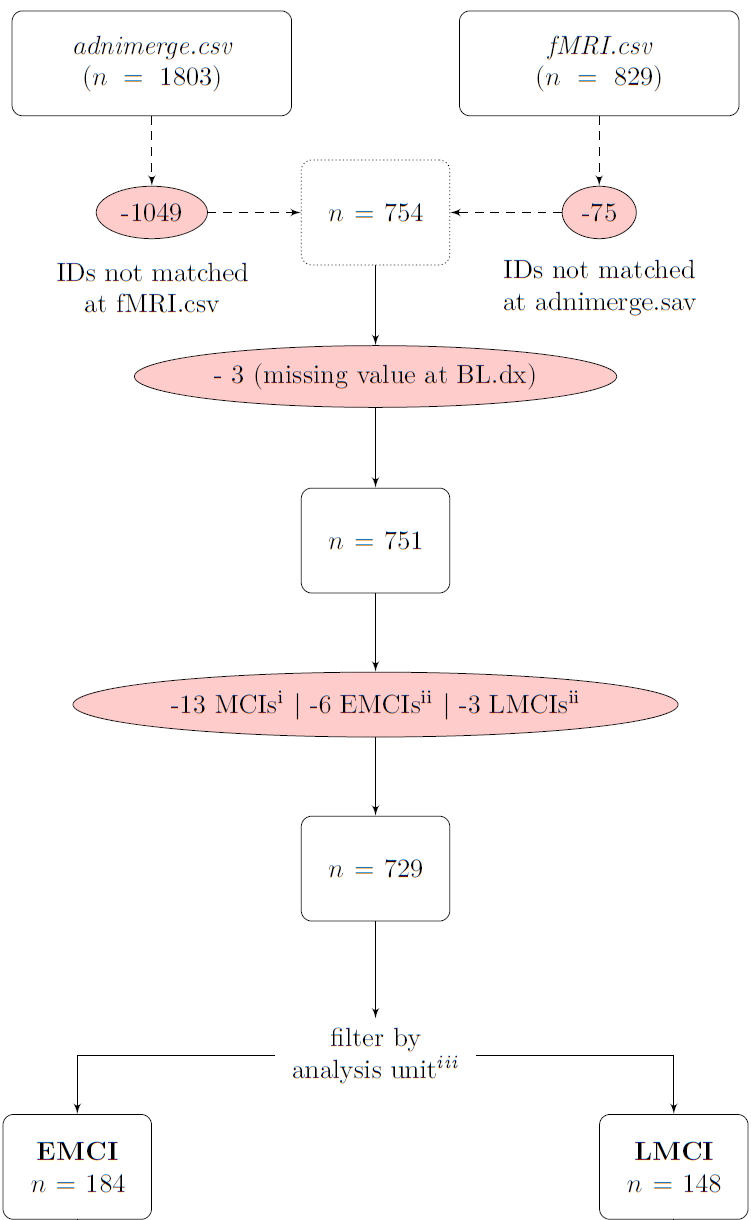
\includegraphics[width=0.8\textwidth]{fig_inclusion_datalinkage.png}	
		\caption{\textbf{Flow chart of participants from the initial step of the linkage process until the definition of our 332 eligible participants} (See RECORD guidelines 6.3 item for more information).\cite{Benchimol2015} $|$ $^i$ We excluded these 13 patients (see annex for identifiers) since they had an MCI label in the diagnosis ($DX$) variable. Since data from the ADNI go$/$2 was used, the ``MCI'' diagnostic was not expected: this diagnostic was reserved to ADNI 1 (where no fMRIs were registered). Here, only EMCI and LMCI needed to be taken into account. Besides, among those 13, 12 of them did not have any follow-up visit; and the one that is left did only have a baseline visit and only one follow-up visit.  $|$ $^{ii}$ 6 EMCI and 3 LMCI patients were excluded as they did not have any follow-up visit registered in \textit{adnimerge.csv} after the date of the baseline diagnosis. $|$ $^{iii}$ The analysis unit is composed of patients with EMCI and LMCI, which means other categories such as SMC (significant memory concern) and CN (healty controls) are not included in our analysis unit or eligible population.}

		\label{fig:data_linkage}
	\end{figure}
	\FloatBarrier	 

	\subsection{Inclusion and exclusion criteria} \label{sec:inclusion_exclusion_criteria}
	
	Among the sample specified in the last subsection \ref{entry_criteria_and_setting} we separated between those who evolve from EMCI or LMCI ($dx=2$) to Alzheimer's disease ($dx=3$), from those who do not convert to AD across time ($dx=2$ to $dx=2$ as long as the follow-up lasts, for stable; or $dx=2$ change to $dx=1$, for remissions). The former were labeled as \textbf{MCI-c} or MCI converters, and the latter were labeled as \textbf{MCI-nc} or MCI non-converters (see figure \ref{fig:conv_no_conv}).
	
	\begin{figure}[h]
		\centering
		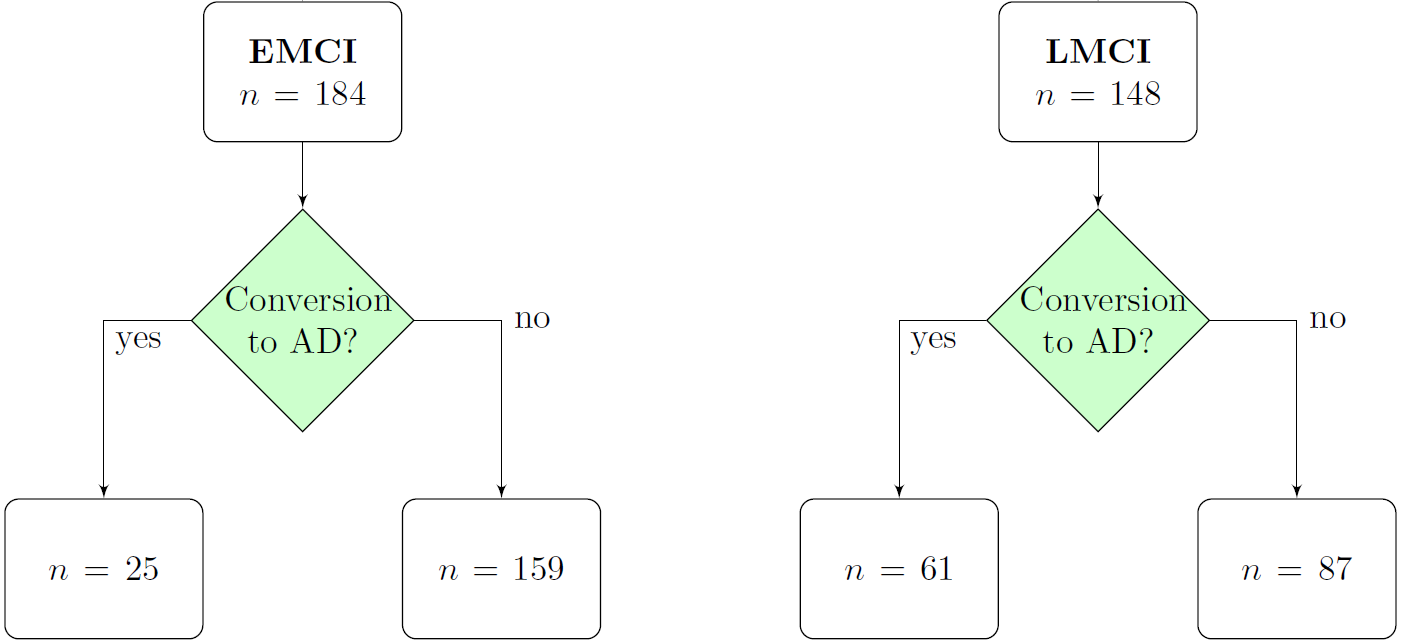
\includegraphics[width=\textwidth]{fig_conv_no_conv.png}
		\caption{Identification of MCI converters and MCI non-converters}
		\label{fig:conv_no_conv}
	\end{figure}
	\FloatBarrier
		
		
	In the previous 332 patients the following \textbf{exclusion criterion and inclusion criteria} were then applied\footnote{The resulting final sample is  thoroughly reported in the results section.}, as follows:	
	
	The \textbf{exclusion criterion} was only applied to those subjects who had an AD diagnosis at some point, namely those that we want to label as MCI-c, and it served as a tool to increase the validity of the MCI-c label/diagnostic. For those subjects, we simply want to increase the probability of ensuring each participant actually has converted to AD and that the AD label is not just an incorrect diagnosis preceding a \textit{regression toward the mean} phenomenon. In order to do that we took the following approach: if the participant had shown a manifest \textit{inconsistency} across the follow-up diagnostics, then we removed them from our sample. We have chosen to define this inconsistency by giving it two alternative definitions: one is the presence of two or more consecutive follow-up visits with a diagnostic that is less severe than the AD one (either MCI or healthy) in the subsequent follow-up visits held \textit{after} the visit in which the subject received the AD diagnosis (e.g, $MCI \rightarrow MCI \rightarrow AD \rightarrow MCI$ would still be considered consistent so the subject would not be eliminated, whereas  $ MCI \rightarrow MCI \rightarrow AD \rightarrow MCI \rightarrow MCI$ would already be considered inconsistent due to the aforementioned \textit{regression toward the mean effect}) \textit{or} as an oscillating pattern of diagnosis across the follow-up visits ($MCI \rightarrow AD \rightarrow MCI \rightarrow AD \rightarrow [...]$). AD is not a disease with possibility of remission so basically this is a very important aspect to take into account when considering the quality of our data.
	
	\noindent The \textbf{inclusion criteria} were defined as follows:
	
	
	
	
	\textbf{a)} Participants that have an fMRI scan of the same submodality. Specifically rsfMRI (resting state fMRI)\footnote{The rsfMRI scan is taken while the subject is task-free.}.
	
	\textbf{b)} At least 80\% of the scans, within each study group (MCI-c and MCI-nc), will be acquired within a minimum of a \textit{$\pm 2 $ month interval} from the baseline diagnostic (except for those ADNI 1 participants who continue to ADNI 2 or ADNI GO, who will not be considered for the percentage\footnote{Since fMRI scans are only acquired in ADNI GO, 2 and 3 (thus no fMRI scans were taken at the moment of the baseline diagnostic for ADNI 1 patients) then the differences between the scan acquisition time and the baseline diagnosis for ADNI 1 individuals who are transfered to posterior study stages is going to be huge -5 years or more-. Therefore, for those individuals, the thresholded difference was simply not applied.}).
	

	
	 \textbf{c)}  MCI-nc individuals must have been in a minimum of \textbf{$n$ years of follow-up}. The value $n$ will be obtained by sorting in descending order follow-up times in MCI-nc and eliminating those subjects whose time value is below the mean time of conversion for MCI-c + 0.3 standard deviations (this threshold has been chosen as it gives a good balance between potential validity and sample size). Although mean MCI-c time\footnote{Time origin or time = 0 is at baseline time.} of conversion since baseline diagnostic ($x$ = 2.3 years; $s$ = 1.85) is already below the mean MCI-nc time of follow-up since baseline diagnostic ($x$ = 4.69 years; $s$ = 2.357) (\footnote{p-value from a two-tailed independent samples t-test. Normality of both distributions was assumed.}$p<5.83-e^{16}$), when we subsample our 332 patients under the inclusion criterion a)\footnote{Within the 332 patients, not all of them have received fMRI in the same submodality.} we cannot then be sure that the MCI-nc group will still have a considerably larger number of subjects with follow-up times greater than the conversion time in MCI-c group (if the reader sees figure \ref{fig:compara_distribucions_conversio_followup} they will realize this may be the case after inclusion and exclusion criteria, since both distributions partially overlap). That's the reason why we have just imposed a cut-off point or threshold value for (MCI-nc) follow-up time. This way we then can make sure the classifiers (prognostic models) will be trained upon MCI-nc subjects that, on the one hand, do represent the typical MCI individual who does not convert to AD in a reasonable amount of time and, on the other hand, we will also be sure of not including data to develop our model with MCI-nc patients with follow-up times below the average time of conversion to AD in the MCI-c group. With this, we will drop the chances of including subjects that could have been categorized, if followed longer, as MCI-c instead of MCI-nc (subjects that, methodologically, would be false negatives of the labeling process): something that would induce bias to our predictive models since some outcome information could then be potentially invalid.
	
	Note we do not cut the right tail of the MCI-c conversion time distribution since we have an imbalanced dataset and MCI-c is the underrepresented category. You can see both distributions for the 332 eligible participants in figure \ref{fig:compara_distribucions_conversio_followup}.
	
	
	\begin{figure}[h]
		\centering
		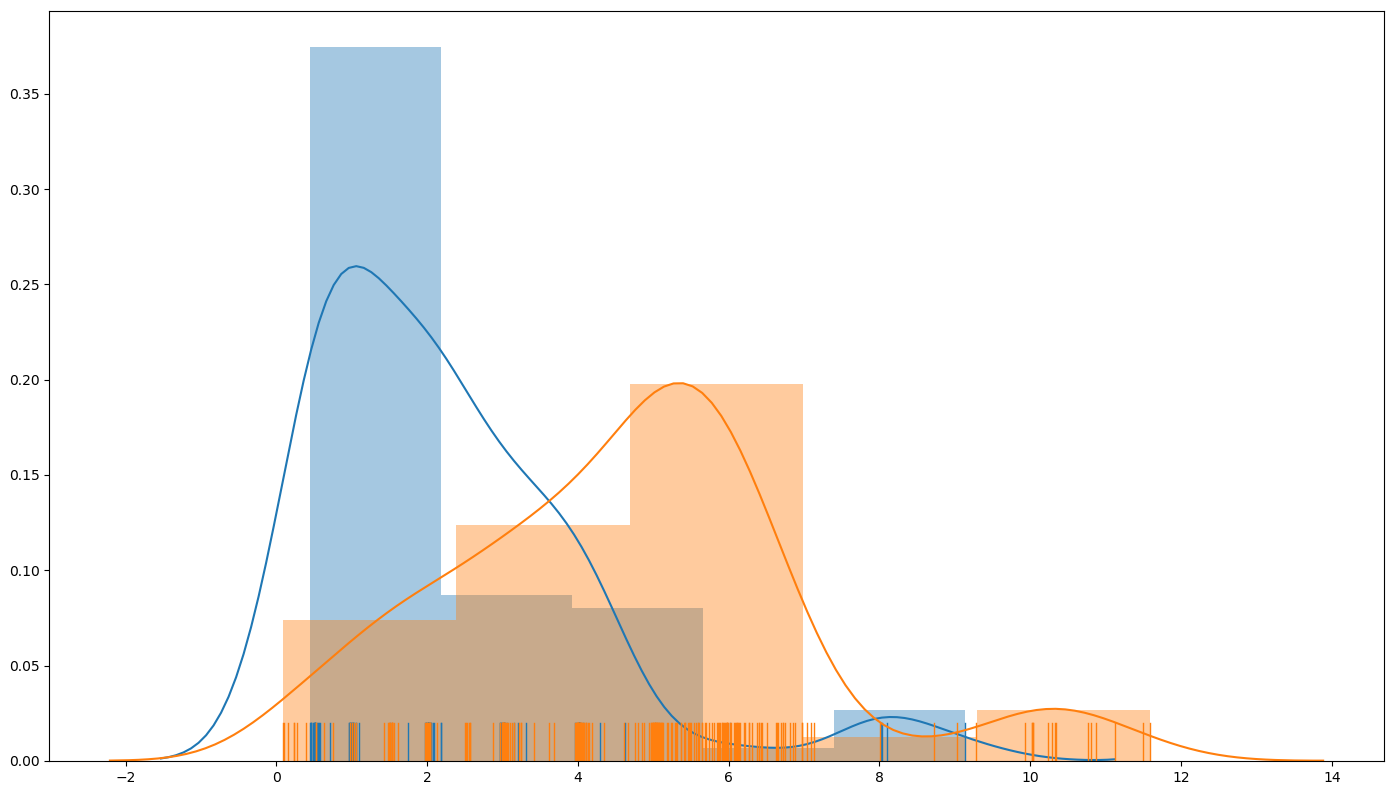
\includegraphics[width=\textwidth]{compara_distribucions_conversio_followup.png}
		\caption{\textbf{Comparison of elapsed time from baseline to conversion in the MCI-c group (blue) and from baseline to end of follow-up in the MCI-nc group (orange) in the 332 patients sample.} $|$ X-axis: time (years) $|$ Y-axis: subject-count.}
		\label{fig:compara_distribucions_conversio_followup}
	\end{figure}
	\FloatBarrier
	
\textbf{d)} Among this sample, at least 80\% of the individuals need to have either CSF total tau, CSF phosforilated TAU, CSF A$\beta $ or ADAS or MMSE scores in order to allow a multimodal approach according to \textbf{\textit{$H_{2}$}.}.

	
\section{Longitudinal follow-up and how data is used with model development} \label{sec:explicacio_tresvisites_screening_baseline_followup}

	
Since we want to do a prognostic study (see section \ref{study design}) it is important to define how we will make use of longitudinal data of the ADNI.

First off, there is the need to clearly define which of the assessments we are interested in are being held in each stage of the study. In order to do that, we can establish three types of visits in the ADNI. Namely, \textbf{the screening visit}, \textbf{the baseline visit} and \textbf{the follow-up visit}.
		
The \textbf{screening visit} (see page 21 of the ADNI2 protocol extension\cite{adni2_protocol_extension} for more information) is the first visit. Its purpose is, on the one hand, to determine eligibility for the proposed study and, on the other hand, to collect measures that will be used as a reference to assess change. A standardized evaluation is performed at each clinical site (demography, MMSE questionnaire, obtaining consent, among others). If (and only if) the subject meets the inclusion and exclusion criteria of the ADNI it will then \textit{a)} receive, in this same visit, a \textbf{3T MRI scan session} and \textit{b)} move on to the \textbf{baseline visit}.
		
The \textbf{baseline visit} (See page 22 of the ADNI2 protocol extension\cite{adni2_protocol_extension} for more information) must take place within the next 28 days of the screening visit. In this visit the MMSE is administered again, a lumbar puncture is made to collect CSF and basically the initial diagnosis (in the cohorts we are analyzing is either EMCI or LMCI) is then well established.
		
The \textbf{follow-up visits} are all scheduled counting from the baseline visit. At month 3 no clinical assessment is made (only another MRI scan is taken). At months 6, 12, 24, 36 and 49 clinical assessments are made and a diagnosis is drawn and registered in the $DX$ variable of the adnimerge.csv. Similarly, the gaps among clinical assessments (usually one year) are covered by telephone assessments at 18, 30, 42 and 54, but no diagnosis is registered.
		
To sum up, the diagnosis that is made at the baseline visit (variable $DX.bl$ of the \textit{adnimerge.csv} file) is, later on, being reassessed  at each follow-up visit that involves contact with clinicians (see figure \ref{fig:seguiments_metode}).
		
		\begin{figure}[h] 
			\centering	
			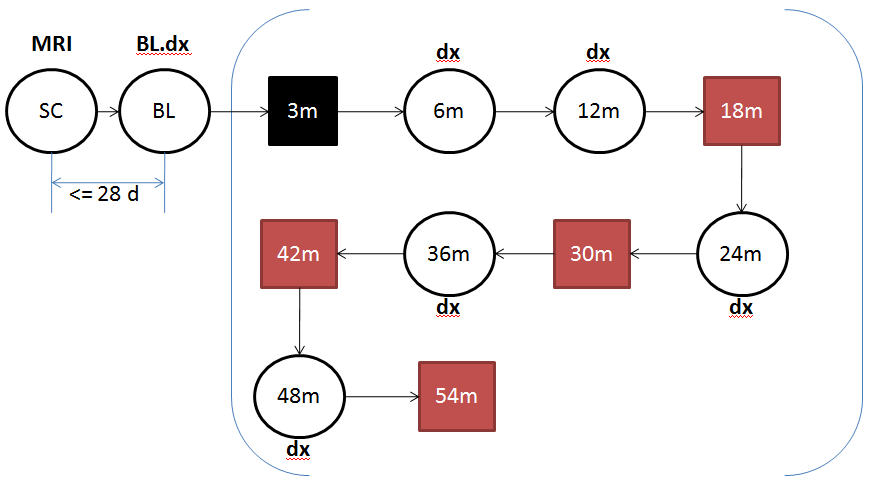
\includegraphics[width=\textwidth]{fig_seguiments_metode.png}	
			\caption{Screening, baseline and follow-up visits in the ADNI. Red squares are phone visits. Circles within the claudators are clinical visits, where diagnostic is drawn (variable dx). SC and BL stand for screening visit and baseline visit respectively, where the baseline diagnosis (BL.dx) is established.}
		\label{fig:seguiments_metode}
		\end{figure}	
		 
	
Now that we have defined how is the data collection made at the ADNI we will state when do we collect the data we need to answer our study hypothesis. See the following \ref{measures} section.




%TPROTOCOL
\section{Measures} \label{measures}

	\textbf{Outcome:} Conversion or not conversion to the Alzheimer's disease.
	
	\textbf{Main predictor:} BOLD time-series intra-subject correlations or, simply, functional connectivity (see this concept explained at the statistical analysis section: \ref{estadistica-fcon}) 
	
	\textbf{Candidate predictors:} total tau in CSF, phosphorialted tau in CSF, 	$a\beta$\footnote{Ideally we would like to have $a\beta_{1-42}$ since it is the protein that has shown best predictive behaviour. However, in the ADNI we have only general CSF $a\beta$ protein levels.}, ADAS and MMSE scores.
	
	As we stated in the study design section \ref{study design}, we retrieve the main predictor cross-sectionally: only at the screening visit of the ADNI (imaging biomarker, fMRI), or at the baseline visit of the ADNI (for the fluid biomarkers and/or neuropsychological tests if \textit{\textbf{H2}} model  is tested), both within 28 days of difference. We assess the presence or not of the outcome at every follow-up visit for each participant, as long as it involves clinical assessment (i.e. not phone interviews, where no follow-up diagnosis is made): that means at month 6, month 12 and then on a yearly basis until either conversion to AD or subject withdrawn from the follow-up visits are produced. Thus, this basically means we assess conversion at the white circles within the claudators in figure \ref{fig:seguiments_metode}), via a custom Python script\footnote{The reader can access to a subset of the scripts created for this final thesis in \href{http://bit.ly/scripts-sample}{http://bit.ly/scripts-sample}. NOTE: Variable names are in catalan.} applied to the 332 participants from the ADNIMERGE.csv file (see Annex \ref{subsec_appendix_obteniribaixarInfoADNI} for more information).



\section{Statistical Analysis} 


\subsection{Power calculation} \label{PowerCalculation}

We were unsure as to how to calculate the required sample size using standard procedures, such as the GRANMO website\footnote{\href{https://www.imim.cat/ofertadeserveis/software-public/granmo/}{https://www.imim.cat/ofertadeserveis/software-public/granmo/}}, as we did not find ways of creating a priori precision metrics for the most important estimates to be used in our study (specificity and sensitivity). We happen not to find this as a strange situation, since in diagnostic accuracy studies\footnote{This studies have the same estimates than in prognostic studies.} researchers often decide about the sample size arbitrary, either for their convenience or from the previous literature\cite{Hajian-Tilaki2014193}: so prognostic studies are to find the same difficulty, as the accuracy measures to test their models are similar. Furthermore, Hajian et al.\cite{Hajian-Tilaki2014193} make reference to reviews of publications where it has been shown that less than 5\% or less over the total diagnostic accuracy studies published include precision estimates for their accuracy measures (for example, \cite{Bochmann2007898, Bachmann20061127}).

We used the proposed method of Hajian, T. \cite{Hajian-Tilaki2014193} to calculate the expected value of sensitivity (or specificity) that we wanted our diagnostic models to have ($P_{1}$) when comparing it to a pre-determined value of sensitivity (or specificity) we would like to surpass on our sample ($P_{0}$).

In this case, since we anticipated our sample size\footnote{We use the word ``sample size'' instead of ``validation set sample size'' because we do not have an independent validation set. All sample is used both to derive the model and to validate it (several train/test splits are done using a cross-validation -see section \ref{deriv_valid}-).} 
would be rather small we set a realistic threshold $P_{0} = 0.50$ (given we have a binary classification problem, this corresponds to chance level). Then, we set $P_{1} = 0.70$ as the minimum expected value of both sensitivity and specificity\footnote{We fixed the minimum proportion to 70\% since, as a rule of thumb, this is the minimum acceptable value for a diagnostic/prognostic test, something that we believe is acceptable considering the almost non existing literature of prediction of MCI conversion to AD with fMRI -Hojjati et al made the only study that assesses conversion to AD in MCI using rsfMRI, and they found 83.24\% sensitivity and 90.1\% specificity \cite{Hojjati201769}. Thus our estimates are less than optimistic.}.

\begin{equation}
	n = \dfrac{[Z_{\alpha/2}\sqrt{P_{0}(1 - P_{0})} + Z_{\beta}\sqrt{P_{1}(1 - P_{1})}]^{2}}{(P_{1} - P_{0})^{2}}
\end{equation}

When using the specified values, and considering the standard 95\% confidence level (or probability) of detecting differences when those differences actually exist $(1 - \alpha = 0.95)$ and the desired statistical power of being able to say those differences do not exist when they actually do not exist set to 80\% $(1 - \beta = 0.80)$ we obtain $Z_{\alpha/2} = 1.96$ and $Z_{\beta} = 0.84$, respectively:

\begin{equation}
	n = \dfrac{[1.96\sqrt{0.50(1 - 0.50)} + 0.84\sqrt{0.70(1 - 0.70)}]^{2}}{(0.70 - 0.50)^{2}} = 19
\end{equation}

Thus, we knew beforehand that if the diagnostic test got to this 70\% accuracy, it would mean that with 19 people in our sample we would already have lower bonds of the confidence intervals above de chance level. So this is the minimum value of people our final sample needs to have. Actually if we set $P_{1}$ to be 0.65, then the sample size would need to be set to 34. Therefore we tried to anticipate that by considering a least favorable scenario and we set the sample size as minimum as 34 before running our analysis.


\subsection{Diagnostic accuracy measures} \label{subsec:Diagnostic_accuracy_measures}

 The predictive accuracy of the models trained is done using several indexes. Namely: accuracy, sensitivity\footnote{It can also be refered to as \textit{recall} or \textit{True Positive Rate}.}, specificity\footnote{Also called \textit{true negative rate}.}, positive predictive value (PPV)\footnote{Also called \textit{precision}.}, negative predictive value (NPV), Area Under the Receiver Operating Characteristic (AUC), positive (LR+) and negative (LR-) likelihood ratios. All of this measures, although apparently redundant, are important to correctly report binary classification problems \cite{Luo2016}. 
 
 We define their proper calculation as follows, after the corresponding confusion matrix, for a given \textit{testing set} $i$ with a $n$ subset of patients.
 

\begin{table}[h]
	\centering
	\begin{threeparttable}
		%\caption{Confusion matrix for calculating diagnostic accuracy metrics}
		%\label{my-label}
		\begin{tabular}{llccc}
			
			& & \multicolumn{2}{c}{\textit{Reality\tnote{a}}} & \\
			\toprule
			& & Conversion & No conversion &  \\
			\midrule
			\multirow{2}{*}{\textit{Prediction\tnote{b}}} & Conversion & \textbf{TP$_{i}$}  & \textbf{FP$_{i}$} & \textit{TP$_{i}$ + FP$_{i}$} \\
			 & No Conversion & \textbf{FN$_{i}$} & \textbf{TN$_{i}$} & \textit{FN$_{i}$ + TN$_{i}$} \\
			 & & \textit{TP$_{i}$ + FN$_{i}$} & \textit{FP$_{i}$ + TN$_{i}$} & $n$ \\
			\bottomrule
		\end{tabular}
		\begin{tablenotes}
			\item[\scriptsize a]{\footnotesize Ground truth. This is what will happen to the subject ``in the future'' according to the follow up visits.}
			\item[\scriptsize b]{\footnotesize The category for which the classification model assigns a higher probability.}
		\end{tablenotes}
	\end{threeparttable}
\end{table}

The aforementioned confusion matrix and accuracy metrics were obtained for each single type of model (see the type of models we tried in \ref{used_models}) and for each train/test split in each fold of the $k$-fold cross-validation\footnote{Again we refer the unfamiliarized reader to \ref{deriv_valid} and to \ref{deriv_valid} so as they can see how predictive research is done and what is a cross-validation, respectively.}. For example, for a logistic regression, a total number of $k$ logistic regressions are trained and tested, with different subsets of data and a different resulting confusion matrix every time). 

In the end, however, we obtained $k + 1$ diagnostic metrics (i.e. $k + 1$ accuracies, $k+1$ sensitivities, etc...). This happened because we took the average diagnostic metrics after the cross validation. This was done by drawing a final confusion matrix featuring the sum of the aforementioned four variables across all $k$ folds of the cross-validation (see again \ref{deriv_valid}). The final matrix is like the matrix above, but with \textbf{TP$_{i}$}, \textbf{FP$_{i}$}, \textbf{FN$_{i}$}, \textbf{TN$_{i}$} replaced, respectively, by $\sum_{i=1}^{k}\textbf{TP}_{i}$, $\sum_{i=1}^{k}$\textbf{FP}$_{i}$, $\sum_{i=1}^{k}$\textbf{FN}$_{i}$ , $\sum_{i=1}^{k}$\textbf{TN}$_{i}$. 

For example, the average diagnostic metrics after the cross-validation are depicted in results section, in table \ref{table:taula_diagnostic_metrics_fMRI_nodimreduc} and the accuracy metrics obtained at each $i$-th iteration of the $k$-fold cross-validation have been useful to plot the distributions of accuracy, sensitivity and specificity the $k$-testing sets (figures \ref{fig_comparacio_models_fMRI_nodimreduc_ACCURACYPLOT} and \ref{fig_comparacio_models_fMRI_nodimreduc_SENSIBILITATESPECIFICITAT}).


We can now define the accuracy metrics that can be calculated from the aforementioned confusion matrices:

The accuracy can be defined as the total number of cases our prognostic model correctly classifies:

\begin{align}
accuracy = \dfrac{TP+TN}{TP+TN+FP+FN} = \dfrac{TP + TN}{n}
\end{align}

Since the accuracy metric does not separate the performance of our models for ``converters'' and ``non converters'' we define sensitivity, which is the proportion of future ``converters'' a given prognostic model correctly classifies as such; and specificity, which is the proportion of future ``non-converters'' a given prognostic model correctly classifies as such. These indexes are measures of intrinsic accuracy, which means they are not affected by the prevalence of the condition \cite{john2011}:

\begin{align}
sensitivity = \dfrac{TP}{TP+FN}
\end{align}

\begin{align}
specificity = \dfrac{TN}{FP+TN}
\end{align}


In the results section we have also provided Positive Predictive Values (PPV) and Negative Predictive Values (NPV) as well. However, unlike sensitivity and specificity, PPV and NPV are dependent on population prevalence. Thus we have also provided positive and negative likelihood ratios\cite{john2011} (LR+ and LR-, respectively):

\begin{align}
PPV = \dfrac{TP}{TP+FP}
\end{align}

\begin{align}
NPV = \dfrac{TN}{FN+TN}
\end{align}

\begin{align}
LR+ = \dfrac{sensitivity}{1 - specificity}
\end{align}

\begin{align}
LR- =\dfrac{1 - sensitivity}{specificity}
\end{align}

Finally, we have plotted the ROC curve to get the AUC and a measure of balance between sensitivity and specificity. In order to create a ROC curve there is only one requirement: ``That the measurements or interpretations can be meaningfully ranked in magnitude'' \cite{john2011}. If we meet this requirement, then a varying decision threshold can be applied across those measurements enabling us to plot the values of varing $1 - specificity$  in relation to $ sensitivity$. Since machine learning models that classify or predict a binary event take out predictions as binary outputs in the forms of probabilities\footnote{See predictproba function in scikitlearn\href{https://bit.ly/2us8h8s}{https://bit.ly/2us8h8s}} placed on a matrix of many rows as subjects in each \textit{testing set} and as many columns as categories to classify (shape $n \times 2$)\footnote{the first column will be a value with the probabilities $ 1 - p $ of belonging to the category dummy encoded as 0 -in this case not having the disease in the future during the follow-up period- and the right column will be the probability of belonging to the category dummy encoded as 1 -having the disease in the future-: $p$.} we just need to vary the decision threshold across the range of possible probability values of one of the columns. By default, the decision threshold of a classifier with binary outcome will be set to 0.5. Since always $0 \leq p \leq 1$, then first, the threshold value  is varied continuously from $p = 0$ all the way up to $p = 1$, and then any noticeable variation of $1 - specificity$ (in the X axes) is plotted against $sensitivity$ (in the Y axes). 

The points now plotted, when connected with straight vertical and horizontal lines have generated the so-called \textit{empirical} ROC curves\cite{john2011} stated in the results section.


\subsection{fMRI analysis of functional connectivity}\label{estadistica-fcon}


One of the predictors as stated in \ref{measures} is what we have called BOLD time-series intra-subject correlations. This is the name we have found more accurate to describe what is called \textit{functional connectivity}, or simply FC.

Since this text is expected to be read by medical professionals, not neuroscientists, we dedicate this part to make the reader understand, on the one hand, how is the extraction of information from the main imaging modality that will be analyzed in this study (fMRI); and, on the other hand, to show how the data that comes from this imaging modality is used to create a predictive model.

First off, it is known that brain areas where there is higher metabolic activity in a given time also receive a higher supply of oxygenated blood at that time. This brings about deoxygenated hemoglobin changes in blood, which in turn leads the proton signal from the water molecules surrounding the vessels to change \cite{nature_Chou}. The BOLD is a signal whose value changes depending on whether the analyzed area has higher or lower metabolism. Specifically, an increase in the positive BOLD signal in adults generally represents a net increase in neuronal activity\cite{Hall2016}. fMRI scans, which are quite similar to the widely used structural MRI scans in medicine, basically rely on a magnetic field to ``see'' the aforementioned changes in the protons. However, instead of focusing in structure, the fMRI scan focuses in function: it analyses changes in the BOLD contrast in each spatial location of the brain, instead of ``directly seeing'' the brain, and more importantly: the fMRI does it across time.

The same way as a video can be understood as a stack of several bidimensional frames with  $m \times n$ resolution ($m$ rows of pixels by $n$ columns of pixels), a single fMRI image -taken from a single subject- can similarly be understood as a stack of several three dimensional frames with $m \times n \times l$ ``pixels with volume'', also known as \textit{voxels}. Thus, an fMRI image (within one or several .nii or NIFTI file, such as the ones that have been analyzed here) is stored in a multidimensional array or tensor of $m \times n \times l \times frames$ \cite{Larobina2014200}. Now, for each of these voxels we can then associate a time series of the BOLD measure (it is a quantitative continuous variable, with as many values as $frames$ we have registered during the acquisition period of the fMRI scan). However, since a standard fMRI scan can have roughly around one million voxels (usually $ m \approx n \approx l \approx 100 $ then $m * n * l = 1 000 000 $), there is too much data we can understand or even analyze. Hence, this data needs to be reduced: in order to do it we have taken the common approach of spatially parcelate the volumetric information according to a structural brain template or ATLAS, that defines ROIs or Regions of Interest \cite{Rathore2017530}. A very popular atlas is the AAL, a common anatomical parcellation of a Spatially normalized single-subject volume from the Montreal Neurological Institute (MNI), composed of 45 anatomical volumes of interest in each hemisphere (AVOI)\footnote{a)consider AVOI as a synonim of ROI $|$ b) Bare in mind that AAL not only reduces the amount of variables of the fMRI scan, but also makes fMRI scans comparable across all subjects, by warping them on the standard MNI space\cite{Tzourio-Mazoyer2002273}. AAI parcelation is based in anatomy so each of its ROIs might have the risk of mixing time courses \cite{Shen2013403}.} However, the only study that assesses the same question as us has already used it \cite{Hojjati201769}, thus we decided to use a functional connectivity based atlas. We then chose Shen's atlas, which is build based on BOLD signal rather than on an anatomic distinction and generates more accurate and more spacially homogeneous parcellation results for resting state fMRI analysis than the anatomical aproach\cite{Shen2013403}\footnote{Note there are more preprocessing steps to be performed, such as motion correction, slice timing correction, coregistration, segmentation and normalization.}.


Each subjects' fMRI has to be adjusted (warped or normalized) to the atlas. There are several ways of doing that such as the (\href{http://www.fil.ion.ucl.ac.uk/spm/}{SPM package}) for MATLAB; or the FSL software \cite{Jenkinson2012782}, which can be freely downloaded from Oxford University website \href{https://fsl.fmrib.ox.ac.uk/fsl/fslwiki}{website}\cite{oxford_fsl_web}, is open-source and does not rely on third party paid software. We used FSL and you can see the steps in the fMRI Data preprocessing section \ref{fmri_preproc}.
 


Shen's Atlas has 214 ROIs. Thus, parcellation of the roughly one million voxels contained in every fMRI scan, into these 214 ROIs (which act at this stage as variables again) of Shen's atlas reduces the number of variables per subject by a factor of five thousand. With it, computational efficiency when fitting models was expected to be higher as at this step we had ``only'' 214 BOLD time-series for each subject, one for each ROI\footnote{Since Shen's atlas has not anatomically defined regions, those have no names and no direct interpretability; unlike, for example, the AAL whose regions correspond to parts of the brain as you can see in Annex \ref{AAL_annex}.}.

Once data was already parcelled, for each subject we no longer had the previous 4-dimensional array with shape $m \times n \times l \times frames$. We had just shrunk it to an array of shape $frames \times N_{ROI}$. That means we had, for each subject, a 2D-matrix or standard dataset with ``SPSS-like'' or ``excel-like'' appearance, with the 214 regions of interest (placed in columns) and the time-series of the BOLD contrast (placed in rows).

Soon after that, for each subject, we computed the pair-wise connectivities (Pearson correlation values) between the activation (BOLD values) for all pairs of regions of interest \cite{Rathore2017530}. So from a matrix of $frames \times N_{ROI}$ (in this case $140 \times 214$) we obtained a correlation matrix or \textit{adjacency matrix} $ \textbf{A} $ of shape $N_{ROI} \times N_{ROI}$ ($214 \times 214$), where each element $ \textbf{a}_{ij} \in \textbf{A} $  was the Pearson correlation coefficient between the $i$-th ROI and the $j$-th ROI.

Given a set $ k $ of variables is easy to see that if we compute all their possible pair-wise correlations and we organize it in a correlation matrix we will have all the possible correlations either on the lower or on the upper triangle of the correlation matrix. Therefore, after removing the main diagonal (which contains correlations of the variables upon themselves and, obviously, is not useful information) and only retaining the correlations of, say, the lower triangle we get a total number of $(k^{2} - k)/2 = k(k - 1)/2$ pearson correlations. This is the exact approach we took here, and since Shen's atlas contains 214 ROIs we got a total number of $22791$ Pearson correlations\footnote{$(214*213)/2 = 22791$} among all of them, which were flattened on a single vector to. This single vector $\textit{V}_{1x22791}$, which we can call the vectorized functional connectivity, contains all the functional connectivities for a given subject. 

Finally, we repeated this process for each subject in our subsample. Each generated vector was stacked as a row of a new matrix named $\textbf{X}$ that ended up having shape $s \times 22791$ (as many rows as subjects -s- and as many columns as correlations among all ROIs).

Now, this information is the final \textbf{functional connectivity} matrix that we have used as \textit{input} or main predictor for our classification models (in the end the $\textbf{X}$ matrix has shape $57 \times 22791$, according to the final sample after inclusion and exclusion criteria application -see green block in results section figure \ref{fig:fig_tikz_diagramaInclusioExclusio_resultats}-).

\subsection{Building the predictive models}

The predictive models were built in the following way. First, we labeled those EMCI/LMCI patients who converted to AD (i.e MCI-c as a 1), and those who did not convert (i.e. MCI-nc) as a 0 (see inclusion and exclusion criteria for more information \ref{sec:inclusion_exclusion_criteria}). This was our \textit{outcome variable}, the dependent variable or simply the $\textbf{Y}$. The values were encoded as a vertical vector of shape $s \times 1$.

Then, our predictor or independent variable -for the Hypothesis 1- were the functional connectivities (i.e. the $\textbf{X}$ matrix with shape $57 \times 22791$, which contained the vectorized functional connectivities of all subjects, as stated in \ref{estadistica-fcon}).

We then had one matrix and one vertical vector: the $\textbf{X}$ (shape $s \times 22791$) and $\textbf{Y}$ (with shape $s \times 1$). This was all we needed to start doing a cross-validation and train and test our models.

However, before carrying on there is something important we needed to account for: ``feeding'' the model directly with such a great number of independent variables (22791 variables) when training it in each fold is expected to lead to a bad classification performance \cite{Shen2014147}. This problem is also known as \textit{overfitting}. \textit{Overfitting} is a commonly used word in machine learning literature and basically means that the fitted model is not able to generalize to another dataset (i.e. in the each \textit{testing set} of the cross-validation, a low accuracy is expected to be obtained). This would happen because at each training iteration, the number of parameters the model has is much bigger than the number of available data (i.e. people) in each training set. This would be the case here: because we have 22791 variables and, in the end, we are having 57 patients: the number of parameters any classification model will have is going to be far higher than the number of patients.

As a result, in fMRI functional connectivity analysis the data dimensionality tends to be reduced first. That is, we want to find a smaller number of variables that correctly summarizes the initial set of 22791 independent variables we have. Basically, we want a more parsimonious model.

This can be achieved by means of dimensionality reduction techniques, also known as exploratory techniques, or unsupervised learning approaches. Two common and widely used of this techniques are \textit{Independent Component Analysis (ICA)} and \textit{Principal Component Analysis (PCA)}.  Another way of dealing with this problem is to use recursive feature elimination\footnote{https://bit.ly/20Qd50F} by letting the model to choose the best number of input variables for our model, by maximizing classification accuracy.

Finally, once the number of variables or predictors has been reduced, we can introduce the new information into our models, being these new measures paired with the outcomes without being that fearful from overfitting. Therefore, with dimensionality reduction, the model would see $X'$ variables ($X'$ is a reduced matrix $X$ with shape $s \times p$ such that $p \ll 22791$) and the former $Y$ outcome variable values. After that, and after a cross-validation performed using $X$ and $Y$ (details of cross-validation are explained in \ref{deriv_valid}) we will have our diagnostic accuracy results.

In order to ``feed'' each type of model (see models depicted in \ref{used_models}) we have tried both approaches: using the functional connectivities without dimensionality reduction and with dimensionality reduction (both with PCA and Recursive Feature Elimination).




\subsubsection{derivation set, crossvalidation and validation set} \label{deriv_valid}
Before carrying out with the explanation we must introduce some theoretical framework on how correctly a machine learning model or predictive model gets properly trained and validated:


The idea of predictive research is to train models under a dataset (\textit{the development set}) and then see if they generalize under another dataset (\textit{the validation set}). 


Firstly, the model ``learns'' parameters in the development set by ``reading'' or ``seeing'' both the values for the \textit{predictors} and also the \textit{labels} or the values for the \textit{outcomes}. And secondly, the previously trained model is now validated in the \textit{validation set}. The particularity of the \textit{validation set} is that the model is blinded to the values the outcomes contain (it can only ``see'' the values for the predictors). Therefore, in the validation set the model does not change its parameters anymore: it uses its already tuned parameters to
basically estimate a \textbf{probability} for each participant to belong to one of the two classes: for example, either converter (MCI-c) or non converter (MCI-nc). Finally, when the model draws a conclusion in the \textit{validation set}, we compare the output probabilities it gets to the ground truth outcomes, which in this case would be the outcome labels that inform us about whether or not a subject will actually convert to AD in the follow-up time-span, and we obtain the data diagnostic metrics (sensitivity, specificity and so forth).


However, in the final 57 patient sample obtained (see \ref{sec:participants_results_part} for information on it), the sample size is too small to create a validation set. Thus, then we use the development set both to train the model and validate it. In order to do that we have used the procedure called cross-validation, and, more specifically we have used the $k$-fold cross-validation. With this procedure all the data of the final sample (the so-called \textit{development set}) eventually works both as a training set and as a validation set. For that matter, we will not use the concept ``validation set'' but the concept ``testing set'': at the end of a cross-validation, and for each type of model tested, we have performed $k$ \textit{training sets} and $k$ \textit{testing sets}. With this procedure, at every fold or iteration of the process (for i=1 to i=k), each type of model gets trained with $k-1$ subsets of the data and gets tested in the remaining $1$ (being, of course, each of the train/test splits performed at every fold of the cross-validation \textit{disjoint} sets). This, therefore, implies that for each type of trained model we will need to actually train iteratively $k$ models and only after getting their accuracy metrics averaged or their distributions plotted (you can revisit \ref{subsec:Diagnostic_accuracy_measures}) we will have an idea of how well it performs.


In each of the folds, we have stratified by category or outcome \cite{Luo2016} (converter or non-converter) using the \textit{StratifiedKFold} method from scikitlearn \footnote{\href{https://bit.ly/2L3LIdR}{https://bit.ly/2L3LIdR}}. Under the scope of each fold of the cross-validation, if $n$ is the quantity of people available in our final sample, a proportion $n/k$ of patients randomly went to the \textit{test set} and $nk/(k-1)$ to the \textit{training set}.

This process, performed in this final thesis, is depicted in the left claudator of figure \ref{fig:cross_validation} and we have given $k$ the value \textbf{10 (10-fold cross-validation)}. In this same figure we explain how ideally this process should be performed: In this case the our 57 patient sample acted as a ``development set'' where we performed a cross-validation within it.

\begin{figure}[h] 
	\centering	
	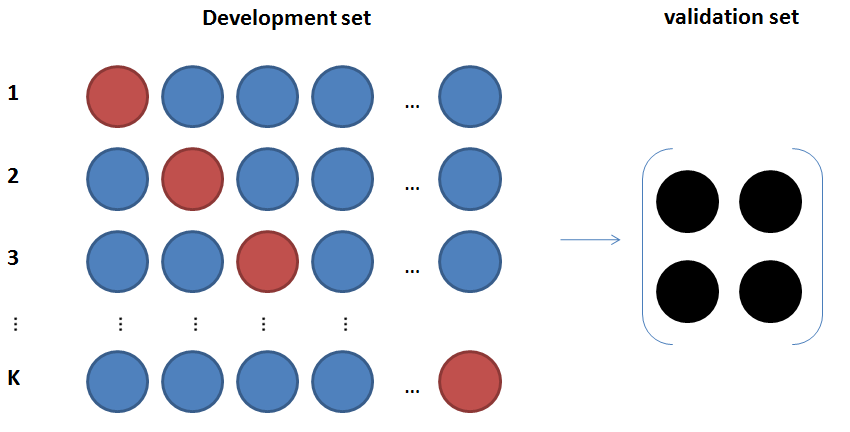
\includegraphics[width=\textwidth]{fig_cross_validation.png}	
	\caption{k-fold cross-validation for our sample, that acts as a \textit{development set}. In each line, the blue sets are used for training the model, and the red ones for testing it. In ideal conditions, the best performing model out of the \textit{development set} should be tested on a validation set if the sample was big enough (which is not the case here).}
	\label{fig:cross_validation}
\end{figure}

\FloatBarrier

A common approach of cross-validation is the leave-one-out cross-validation (LOOCV). However, this approach leads to unstable and biased estimates\cite{Varoquaux2017166}, and the 10-fold cross-validation is recommended over it. Other alternative methods, such as Bootstrap .632+, can also be used, but in certain situations appear to be more biased than the 10-fold cross-validation\cite{Kim20093735}. Thus, we decided to use the 10-fold cross-validation.


As we said earlier, when we apply a technique to avoid overfitting, there are certain parameters of our model that need to be changed after we have trained our model. An incorrect approach would be to test the model several times and tweak it until we got the desirable results. This would be a methodological mistake in which we could have data leakage, which is the unintended use of data the model should not be seeing \cite{Luo2016}. Data leakage is a common problem in studies relying with neuroimaging data \cite{Kriegeskorte2009535}, so special care needs to be taken to prevent it\footnote{This is actually the main problem we have found in the only study that tries to answer our exact same prognostic question\cite{Hojjati201769}.}. This is something that can be solved doing a k-fold cross-validation. Since, at the end of the process, all the data has served both as a train instance and as a test instance the byproduct of that is we have been able to use all the data available in our sample but, at the same time, without having a high risk of bias due to data leakage. 











\subsubsection{Candidate models} \label{used_models}


We have tried different machine learning models or classifiers. Namely, \textit{binomial Logistic Regression}, \textit{Support Vector Machines (with linear Kernel)}, \textit{Artificial Neural Networks (Multilayer perceptron)}, \textit{Nearest Neighbours} and \textit{Gaussian Naive Bayes}. In each fold of the Cross validation, they were all fitted both without previous dimensionality reduction and with dimensionality reduction (\textit{PCA}) of the data. All those models have been tested with no regularization and or no hyper parameter tuning -no grid search- due to the lack of an \textit{internal validation set} (see \ref{deriv_valid}). This has been achieved both by leaving all parameters in default values for the standard classifier objects of the sci-kit learn library and by refusing the possibility of doing grid search\footnote{It denotes the iterative process of training and testing the model several times and, at each iteration, twick its hyperparameters until diagnostic accuracy is maximized.}, in an attempt to avoid data leakage from the training to the testing data (see \ref{deriv_valid}) and cope with the absence of an independent validation set than the one used to develop the models via cross-validation. When doing predictive research regularization helps us avoid over-fitting \cite{Arbabshirani2017137}, but in this case finding solutions for overfitting was not a methodological sound possibility.

The model with better diagnostic performance has been the multi layer perceptron or MLP, so we will make a brief definition of it:

The MLP is a type of Artificial Neural Network that is comprised by one input layer (with as many ``neurons'' as input variables or features), one output layer (with as many ``neurons'' as output categories) and 0 or more hidden layers. Between each of the layers there is a matrix multiplication followed by a non-linear activation function -here, the ReLu function is used, also known as the rectified linear unit-.

The version we have used here has only one hidden layer. Thus the neural network can be represented as follows:

\begin{figure}[h] 
	\centering	
	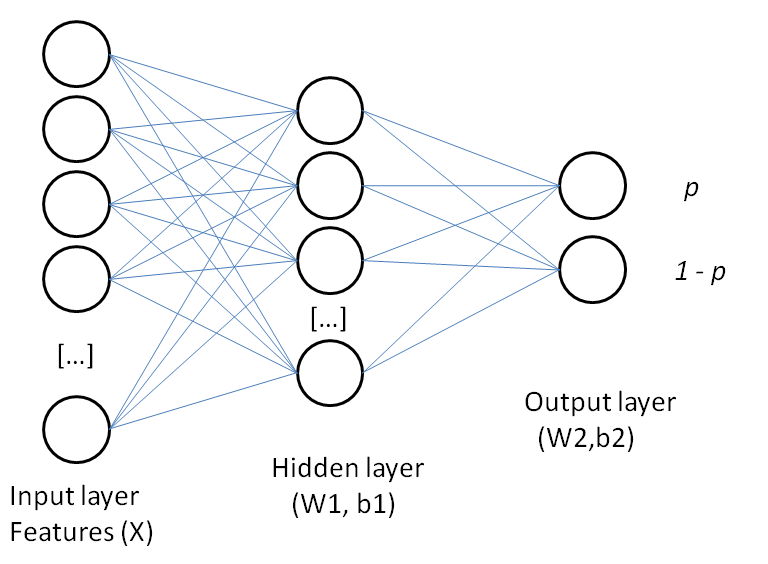
\includegraphics[width=\textwidth]{fig_MLP_neurones.png}	
	\caption{The representation of a MLP with one single hidden unit.}
	\label{fig:calibration_vs_no_calibration}
\end{figure}


More analitically it can also be represented as the series of matrix operations and non-linear transformations involving parameter estimation of matrices of weights (W) and vectors of biases (b)\cite{tfWithoutphd}:

\begin{center}
$Y1 = ReLu(X$·$W1 + b1)$\footnote{A function that maps positive values to the identity function, and negative ones to zero.}
\end{center}

\begin{center}
$Y2 = Softmax(Y1$·$W2 + b2)$\footnote{Softmax is a type of logistic regression.}
\end{center}

Here the input matrix is X, with shape $s$·$22791$ and the final output is Y2, with shape $s$·$2$. Y2 contains, in each row, $p$ and $1-p$ output predictions in forms of probabilities.






\subsection{model performance: other metrics}

Besides reporting the diagnostic accuracy metrics, as an overall performance metric for the models generated we have reported Brier scores \cite{Waljee2014, Gerds2008457}.\footnote{We would have liked to report the Hosmer-Lemeshow ``goodness-of-fit'' test \cite{Luo2016, Waljee2014, Steyerberg2010128} with which calibration can be assessed, but no libraries of python were found that implemented this procedure and its complexity made it pointless to be implemented.} 

Calibration can be understood as the confidence of a single prediction. If a model is properly calibrated, when it raises a forecast in terms of a probability $p$ for a given test subject to be ill, then the chances of that subject to be actually ill are to be around that number. Conversely, if it raises a forecast of $\textit{1}-p$ probability of not being ill, the chances of not being ill are to also to be around that value. Logistic regression, by default, shows almost a perfect linear relationship between the fraction of true positives and true negatives and the class prediction probabilities $p$ the model returns, even without calibrating it; however, in other machine learning models, such like the Support Vector Machines, Naive Bayes or Random Forest this is something that does not happen\cite{sklearn-calibration} (see figure \ref{fig:calibration_vs_no_calibration}). Calibration requires a different set of data than the one used to train the model\cite{sklearn-calibration}. We do not have this data, thus Brier Scores will not be an indication of actual model performance, but an indication of both model performance and calibration.

\begin{figure}[h] 
	\centering	
	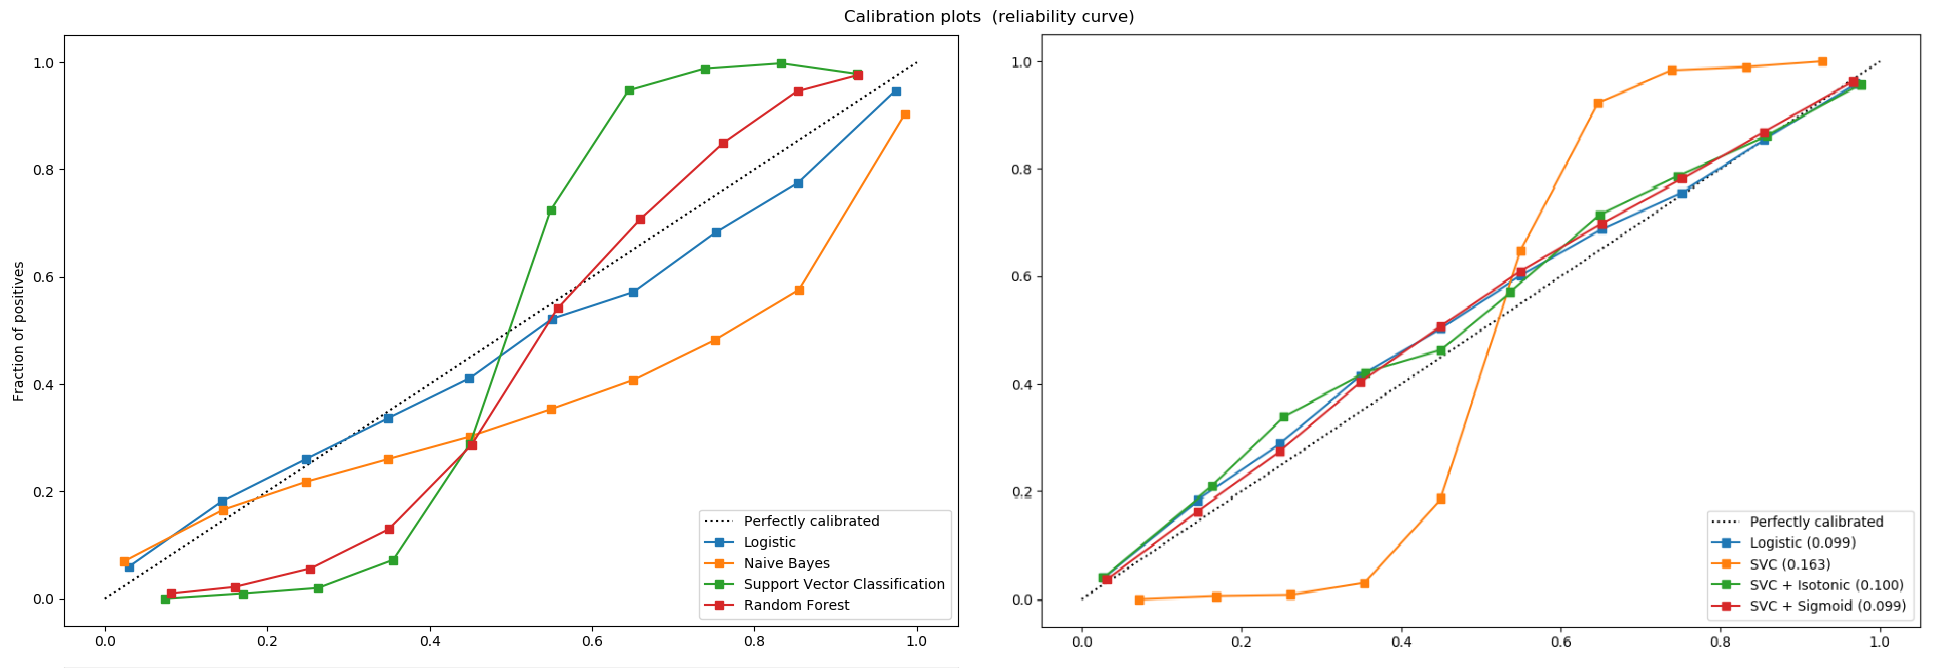
\includegraphics[width=\textwidth]{fig_calibration_vs_no_calibration.png}	
	\caption{Left graph depicts the calibration plot before calibration, and right graph after model calibration. These calibration plots show the prediction probabilities raised by certain machine learning models of a subject belonging to a certain category (x axes) and fraction of subjects actually belonging to that category. Logistic regression is the only model that does not require a calibration to give almost perfectly calibrated forecast probabilities. Support Vector machines (Support Vector Classification or SVC) are the model that has the higher need of calibration. Adapted from scikit learn website \cite{sklearn-calibration}.}
	\label{fig:calibration_vs_no_calibration}
\end{figure}

Brier scores\footnote{Brier scores can  be compared to the determination coefficient ($R^{2}$) of a linear regression, but with the difference that Brier Scores are to be used on categorical dependent variables instead of quantitative ones.}, can be defined as the squared distance between the patients observed status and the model predicted probability \cite{Gerds2008457}. In a binary classification problem where we have $n$ subjects, we can define it as the average of all the $n$ squared differences between each probability $p_i$ the model returns (where $0 \le p_i \le 1$) and the actual outcome -gold standard, ground truth lavels- $o_i$ (either 0 or 1) known for that subject $i$ respectively, thus, generally the lower the Brier Scores are, the better. Analytically, for these $n$ subjects within each $i$-th iteration of the cross validation, we will have $n$ forecasts $p_{1}, p_{2}, ... , p_{n}$ (see \label{study design} and also $n$ outcomes $o_{1}, o_{2}, ... , o_{n}$. Thus, brier scores can be expressed as:

\begin{align}
	BS = \frac{1}{n}\sum_{i=1}^{n} (p_i - o_i)^{2}
\end{align}




\subsection{Software}

In order to both write this thesis and do the analysis we have relied upon free software. All graphs, statistical analysis\footnote{There is an exception: chi-square tests have been carried out in SPSS 21 due to lack of expertise in scikit-learn.}, and machine learning procedures have been performed using Python3 programming language (3.6.4. version) via scientific computation libraries installed on an anaconda's environment\footnote{https://anaconda.org/anaconda/python} (version 5.1.0) under a Windows operating system. These packages are matplotlib/seaborn\footnote{https://seaborn.pydata.org/api.html}, scipy\footnote{https://www.scipy.org/} and scikit-learn\footnote{http://scikit-learn.org/stable/}, respectively. 

SPSS 21 has been used to access the \textit{adnimerge.sps} syntax file, which allowed us to access the variable names and variable descriptions contained within it; and also to compute $\tilde{\chi}^2$ tests. 

\href{https://fsl.fmrib.ox.ac.uk/fsl/fslwiki}{FSL}\cite{oxford_fsl_web, Jenkinson2012782} has been used for data preprocessing (specifically we used two tools within the program: \href{https://fsl.fmrib.ox.ac.uk/fsl/fslwiki/MELODIC}{MELODIC}\cite{melodic_web} and \href{https://fsl.fmrib.ox.ac.uk/fsl/fslwiki/FLIRT}{FLIRT}\cite{flirt_web, Jenkinson2001143, Jenkinson2002825}) under a Linux distribution platform (Ubuntu). For more information on the usage of those programs, see \ref{fmri_preproc}.

\subsection{fMRI Data preprocessing}	\label{fmri_preproc}

We performed fMRI data preprocessing of a total number of 93 rsfMRI scans (see participants section at section \ref{sec:participants_results_part}). 

First off we used \textbf{Melodic}. For each subject we had a total of 140 .nii files (one per each volume, in a single timepoint), and in order to have each subject session's data into a single file, we used an FSL utility called \textit{fslmerge}\cite{melodic_web}, which consists in a series of commands written in shell scripting language (.sh extension) with which every single subject can have their corresponding 3D tensors merged into one single NIFTI 4D file. Then, using the Melodic Graphical User Interface we did the following procedures, in order:


Firstly, under the data tab, we forced the TR (time elapsed between successive fMRI volumes being scanned) to be 2s. We use the word `forced' because there was an inconsistency between what FLIRT GUI displayed as the actual TR of the images, 1 second, and 3s the TR time that each fMRI scan was supposed to have according to the corresponding .xml files (see \ref{sourceofdata}), which were all 3 seconds. Since all scans where preprocessed assuming the same TR, there are not biases associated with it, because changing the TR only alters the measurement units of the time series plots\cite{melodic_web}. Under this same tab we chose not to trim any volumes: although the rule of thumb is to delete the 5 first volumes of each subject scan, we did not do so because at the moment we considered that it was more important not to reduce the number of time series (see limitations section \ref{limitacions} for more information on that), and we also left the high pass filter cutoff value as default. Secondly, under the pre-stats tab, we motion-corrected the data using all values as default. Thirdly, under the registration tab, we registered the subjects in the Shen standard space\cite{Shen2014147} which, as we stated previously, maps the brain into 214 nodes or ROIs. Finally, under the stats tab, we unmarked two check-buttons: variance-norm and automatic dimensionality estimation. Finally, in the post-stats tab we unmarked the option threshold IC maps.

It is also worth noting that during and after the pre-stats and registration procedure, a $report.html$ file is generated and can accessed with a regular internet browser to see important information related to both motion correction and atlas registration. For the former, the step of motion correction, it is important to make sure the subjects have not had very large translation or rotation changes in position while they were laying within the scans: that is, they should not move above an accepted threshold of mean displacement, an index that includes both translation and rotation (although we were advised to eliminate those scans who had mean absolute displacements of more than 2 mm, since they cannot be properly motion corrected, we didn't have to: no scans needed to be eliminated because the quality of fMRI data in that regard was absolutely perfect). For the latter, the registration procedure, we simply needed to make sure that each scan was perfectly aligned with the standard Shen's space by seeing a graphical representation of the brain template being overlapped by the actual scan (if a subject did not appear aligned, they would have been eliminated\footnote{We found no subjects to eliminate for that reason whatsoever.}). In annex section \ref{meandisplacements_registre} you can see an example of one of these subjects to observe its mean displacements (figure \ref{fig_mean_displacements_annex}) and its correct alignment with the template brain  (figure \ref{fig_registre_cervellets}).

Finally, there is one aspect left to cover. Among these 93 subjects, there were seven of them who had more than one rsfMRI scan taken over the same day. Since our model required only one scan per subject, we ended up deciding which scan to choose by taking the one who had the lowest absolute mean displacements. In annex \ref{escollir_escaners_repetits_dun_mateix_dia} you can see which subjects had more than one scan, the exact values of mean absolute displacements for each of those scans (scan UID) and the reasons for direct exclusion or inclusion of them.



\section{Missing data} %tant tripod com 

No problems with missing data were found while registering the scans to Shen's Atlas. Before doing functional connectivity analysis we checked each ROI for each subject to see if there were any missing values using a custom python script. We did not find any problems with missing data in the BOLD time-series.

Biomarker and neuropsychological missing values have been handled in different ways depending on the type of analysis intended. On the one hand, in order to do table \ref{table:demografics_biomarc_clinic_participants}, where 13 group comparisons took place, we simply dropped the NaN values since we did not need to preserve all subjects. On the other hand, we decided that to create the machine learning Biomarker models / questionnaire models to be combined with the fMRI driven machine learning models, we needed to have the exact same number of output probabilities (predictions) for the former and for the latter (because they are combined). We were considering \textit{mean imputating} those missing values within each study group (that is subjects with missings in MCI-c would be filled by taking the mean within MCI-c group; and missings in MCI-nc would be filled by taking the mean within the MCI-nc group).







































\clearpage 
\part{Results}

	\section{Participants} \label{sec:participants_results_part}
	
	\begin{figure}[h]
		\centering
		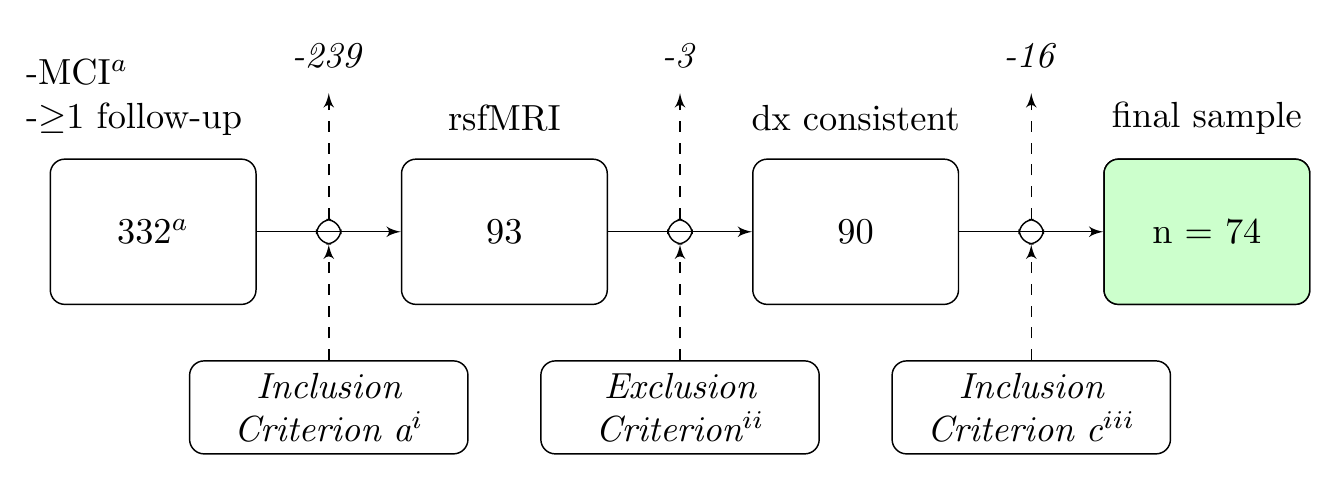
\includegraphics[width=1\textwidth]{fig_tikz_diagramaInclusioExclusio_resultats.png}
		\caption{\textbf{Flow diagram of the application of Inclusion and Exclusion criteria until we get to the final sample (green box).} $| ^{a}.$ Among those 332 MCI individuals there were 184 EMCI and 148 LMCI. $| ^{i}.$ Only included subjects with the same submodality (rsfMRI).$| ^{ii}.$ Excluded 3 subjects due to inconsistency in the diagnostics as defined in methods section.$| ^{iii}.$ Excluded 16 MCI-nc subjects whose follow-up times were below the decided threshold: 2.855 years.$|$ \textit{NOTE: Inclusion criteria b and d did not lead to a variation in included subjects, so these are not depicted here.}}
		\label{fig:fig_tikz_diagramaInclusioExclusio_resultats}
	\end{figure}


		%  a) recorda que "report the numbers of individuals at each stage of the study"(record)
		As we previously stated, after the entry criteria we had a total of 332 subjects (see bottom of \textbf{figure \ref{fig:data_linkage}} for more information) who had been scanned with rsfMRI, had MCI (either EMCI or LMCI) diagnosis at the baseline visit and a minimum of one follow-up. We filtered down those 332 subjects in the exact following order according to section \ref{sec:inclusion_exclusion_criteria}: First, we applied \textit{inclusion criterion a)} which lead us to obtain a subsample of 93 subjects who had scans from the same fMRI submodality: resting state fMRI (rsfMRI) nearby the moment of the baseline diagnostic (except for ADNI 1 participants, as we stated in the Methods section)\footnote{We only preprocessed the nearest rsfMRI scans (in time) to the baseline diagnosis, for these 93 subjects}. Soon after that, we applied our \textit{exclusion criterion} by which 3 subjects with inconsistent diagnostic follow-ups were excluded (2 subjects were eliminated for presenting an oscillating pattern of diagnosis\footnote{Excluded subjects\footnote{(see exclusion criterion definition \ref{sec:inclusion_exclusion_criteria} to find a definition on inconsistency).} were $019\_S\_4293$ and $031\_S \_ 4947$.} and 1 subject for having two consecutive MCI diagnostics after the diagnosis of AD \footnote{Excluded subject was $031\_S\_4005$.} \textit{Inclusion criterion b)} did not lead to discard any subject since among the MCI-c sample and MCI-nc sample there were a 90\% and a 91\% subjects with a minimum difference of 2 months between the dx.bl and the scan date respectively. \textit{Inclusion criterion c)} lead to the cut-off point of the left tail of MCI-nc follow up time distribution at a value of 2.855 years of minimum follow up since baseline visit. With that, a final number of 74 subjects were included in the analysis\footnote{The 16 subjects who were not included for the aforementioned threshold were:002\_S\_2043, 018\_S\_2138, 013\_S\_2324, 129\_S\_4073, 002\_S\_4237, 019\_S\_4285, 130\_S\_4468, 136\_S\_4517, 013\_S\_4791, 031\_S\_4194, 002\_S\_4219, 002\_S\_4251, 136\_S\_4408, 130\_S\_4605,130\_S\_4925 and 013\_S\_4985.}. \textit{Inclusion criterion d)} did not lead to exclude subjects either, since all 74 subjects had no missings in ADAS scores and MMSE scores, A$\beta$, $p$TAU and total tau were only missing in one MCIc subject\footnote{013\_S\_1186 (not excluded).
		} and in three MCInc subjects \footnote{130\_S\_4883, 053\_S\_0919 and 002\_S\_1155 (not excluded).}, which means that 96\% and 94\% over the total MCIc sample did not have missings in those three variables. You can see this process depicted in the flow diagram in \textbf{figure \ref{fig:fig_tikz_diagramaInclusioExclusio_resultats}}.
	

	
		Clinical features, basic demographics and biomarker information of the final 74 subject sample are depicted in \textbf{table \ref{table:demografics_biomarc_clinic_participants}}\footnote{For deciding whether to choose between a parametric or non parametric alternative several homocedasticity (Levene's Test) and normality (Shapiro Wilk tests) assumptions need to be made, so the reader can go to the appendix \ref{taula_levene_shapiro_demografics} to consult the results of these tests in figure \ref{fig:fig_shapiro_levene_taulaDEMOGRAFICS}.}.  In the final sample we have 23 MCI-c. -patients who evolve to Alzheimer's disease-, and 51 MCI-nc -who do not-. Mean age between groups (73 vs 70.7; $p = 0.21$), which is a preliminary indicator that age, indeed, is not acting as a confounder when it comes down to classify subjects\footnote{When doing a classification when finding a variable with no significant differences does not mean this variable cannot help in classifying. To that matter we performed a classification model that did not allow to get a single good classification of diseased individuals (0 sensitivity), so we can consider age not to be a confounding factor.}. Heatmaps for our main predictor, the \textit{functional connectivities}, can be found both for the MCI-c and MCI-nc groups in figures \ref{fig_FC_MCI-c_74sub} and \ref{fig_FC_MCI-nc_74sub}, respectively.
				
		
		
		
		\FloatBarrier
				
		\begin{table}[h]
			\centering
			\begin{threeparttable}
				\caption{Demographic, biomarker and clinical information of our final sample\tnote{a}}
				\label{table:demografics_biomarc_clinic_participants}
				\begin{tabular}{lllll}
					\toprule
					variable\tnote{c} & MCI-c & MCI-nc & statistic (df)\tnote{b} & p-value \\
					\midrule
					n & 23 & 51 & - & -\\
					age&73.0 (7.2)&70.7 (7.1)&1.27$_{t}$ &0.20716\\
					male/female& 11/12&25/26&0.009$_{\tilde{\chi}^2}$(1)&0.924\\
					EMCI/LMCI & 7/16 & 35/16  &  9.421$_{\tilde{\chi}^2}$(1)& 0.002*\\
					follow-up\tnote{d}&1.65 (1.75)&4.61 (1.18)&74.00$_{mw}$&0.00000*\\
					total tau&357.1 (150.3)&270.1 (129.4)&294.00$_{mw}$&  0.00157*\\
					$p$tau&35.7 (17.4)&25.2 (13.8)&270.00$_{mw}$ &  0.00056*\\
					A$\beta$&716.7 (280.1)&1101.7 (418.4)&219.50$_{mw}$ &  0.00005*\\
					A$\beta/p$TAU&26.3 (25.3)&54.6 (29.3)&217.00$_{mw}$ &  0.00004*\\
					FDG&1.2 (0.1)&1.3 (0.1)&-5.21$_{t}$&0.00000*\\
					MMSE&27.7 (1.4)&28.0 (1.8)&492.00$_{mw}$&0.13066\\
					ADAS11&11.9 (4.4)&7.6 (3.5)&4.48$_{t}$ &0.00003*\\
					ADAS13&18.8 (6.6)&12.2 (5.5)&4.46$_{t}$ &0.00003*\\
					ADASQ4& 6.0 (2.9)&4.2 (2.3)&379.00$_{mw}$ &0.00731\\
					\bottomrule
				\end{tabular}
				
				\begin{tablenotes}
					\item[a]{We made 13 comparisons, so to account for multiple comparisons the $\alpha$ = 0.05 decision threshold used to reject $H_{o}$ was modified to be more strict by applying Bonferroni corrections ($\alpha_{corrected} = 0.05/13 = 0.0038$). *means stastistical significance according to the corrected decision boundary. | NaN policy were simply ommited for these tests.}
					\item[b]{For quantitative variables independent samples t-test($_{t})$ was applied, unless either between group homocedasticity and/or within group normality assumptions were violated: then, Mann-Whitney ($_{mw}$) test was employed)¡. For categorical variables we used Chi-squared test ($_{\tilde{\chi}^2}$})
					\item[c]{Quantitative variables are displayed as $mean (s.d.)$}
					\item[d]{Years of followup from the rsfMRI scan until the patient either converts to AD (MCI-c) or loss of follow-up (MCI-nc)}
				\end{tablenotes}
			\end{threeparttable}
		\end{table}
		
			\FloatBarrier	
		
		
	
		
		We happened not to find differences of neither sex ($\tilde{\chi}^2 (1) = 0.009, P = .924$), MMSE scores ($P = .131$) or ADASQ4 ($P = 0.00731$) scores between groups (the latter shows differences but not after bonferroni correct the $\alpha$ level to account for the total 13 comparisons we made in table \ref{table:demografics_biomarc_clinic_participants}). We can explain these absence of differences in MMSE scores because the ADNI inclusion criteria only allowed to enroll participants when their MMSE scores were between 24 and 35 (as we stated in \ref{entry_criteria_and_setting}), which makes the variability of for that variable to be lower. We do find differences in ADAS questionnaire subscales ADAS 11 and ADAS13, by which higher severity scores are found in the MCI-c group  ($P = 0.00003$, $P = 0.00003$, respectively).
		

		
		We find MCI subtype severity differences ($\tilde{\chi}^2 (1) = .9421, p= 0.002$) between MCI-c and MCI-nc groups. This happens because although the number of LMCI is 16, equal for both groups, the MCI-c group has 5 times less patients with EMCI than the MCI-nc group (7 as opposed to 35, respectively). This is not necessarily bad, since EMCI received this diagnostic for having lower Wechsler scale revised score thresholds than the subjects labeled as LMCI at the baseline (as stated in \ref{entry_criteria_and_setting}). This class imbalance is consistent with the idea that the MCI-c group has a worsened condition at the moment of baseline and that they have more chances to turning into AD than their EMCI counterparts. Although we would have liked to have a sample with more EMCI subjects who turn to AD -in order to train and test models with those subjects, whose future disease outcome might a priori be more difficult to predict by a doctor rather than the more severe ones- we understand that this class imbalance could simply be a byproduct of disease nature and, thus, the LMCI stage might even be considered as a prodromal stage of AD, more than the EMCI stage.
		
		A very important variable is the one labeled as ``follow-up'' in the aforementioned table. It gathers the values of effective follow-up time, that is, the time that goes since the moment the rsfMRI scan was taken and the time the subject either converts to AD (MCI-c group) or stops being followed-up (in the MCI-nc group)\footnote{We say effective because before we defined another variable with which ``follow-up'' was considered: the one with which a a cut-off threshold of 2.855 years was established in order to select subjects for our sample. The one we defined before computed the follow-up doing the difference between $baseline diagnostic vs. end of followup"$, whereas now the variable labeled in the table \ref{table:demografics_biomarc_clinic_participants} as ``follow-up'' corresponds to the difference $rsfMRI scandate vs. the end of followup$. In general, using one difference or the other to see the follow up should not add up bias because scans and baseline diagnostics were usually taken with less than a month difference: however, the difference is huge in ADNI 1 participants, whose baseline diagnosis were drawn several years before the rsfMRI scan date.}. In this case the MCI-nc group has an average of 4.61 years of follow up counted from rsfMRI scan dates (i.e. its patients are ``clean'' of AD, on average, for almost 5 years) which contrasts on the mean effective follow-up time of MCI-c (1.65 years). This is interesting since this means that our models span their predictions of future disease (or absence of disease) up until almost a \textbf{5 year range}.
		
		When it comes down to biomarkers, all tau and amiloid biomarkers are different among groups.  On the one hand, $A\beta$ CSF protein levels and $A\beta/p$TAU index are significantly lower in the MCI-c group than MCI-nc at the order of around 1 : 50 000 probability of type I error ($p = 0.00005$ and $p = 0.00004$ respectively). $p$-tau and total tau in CSF are also significantly higher in MCI-c group ($p = 0.0006$ and $p = 0.0016$). Even FDG showed a very significant difference between groups, being lower in MCI-c ($p = 0.00000$). See discussion section \ref{biomarcadors i clinica discussio}.
		
		%FC matrices by group (MCI-C vs MCI-nc)
		\begin{figure}[h]
			\centering
			\begin{subfigure}[a]{0.72\textwidth}
				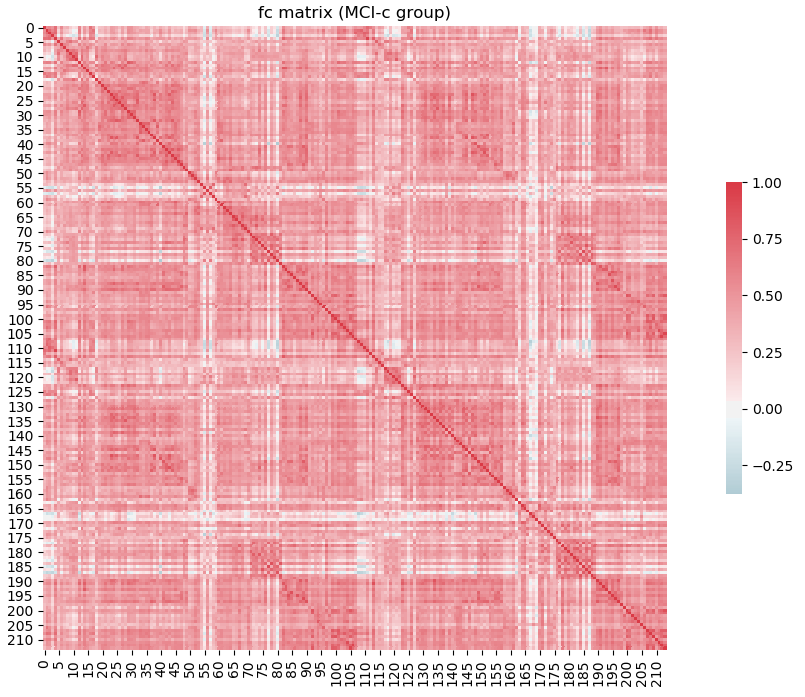
\includegraphics[width=1\textwidth]{fig_FC_MCI-c_74sub.png}
				\caption{Average Functional connectivities in the MCI-c group.}
				\label{fig_FC_MCI-c_74sub} 
			\end{subfigure}
			\begin{subfigure}[b]{0.72\textwidth}
				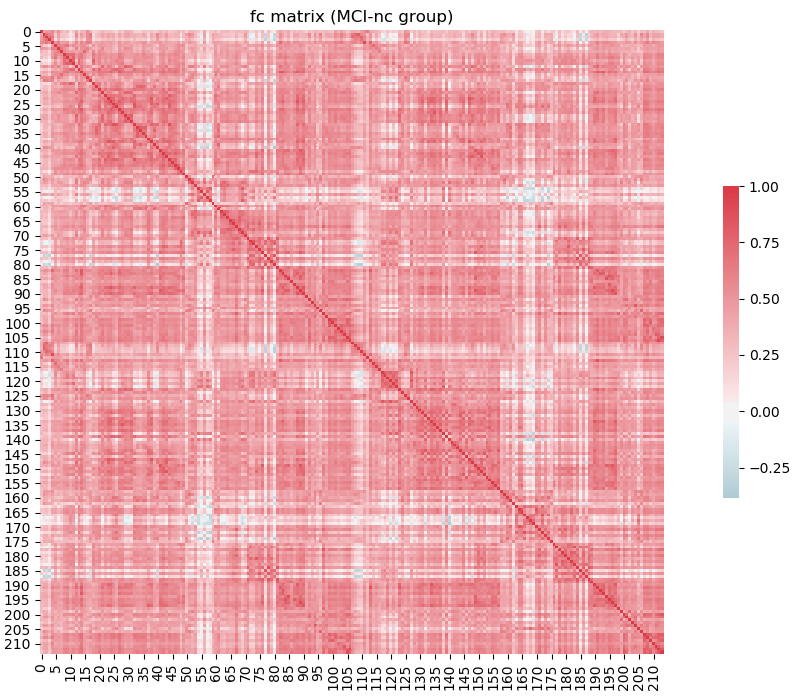
\includegraphics[width=1\textwidth]{fig_FC_MCI-nc_74sub.png}
				\caption{Average Functional connectivities in the MCI-nc group.}
				\label{fig_FC_MCI-nc_74sub}
			\end{subfigure}
			\caption{Heatmap with the average Functional Connectivities per group, across each Shen's atlas node or ROI. No differences are easily found, unlike easier classification tasks such as the one we did with the IDIBAPS dataset (see annex \ref{annex_functional_connectivities}). Here only some increase in the strengh of pearson correlations in the MCI-nc group compared to the MCI-c is found (positive correlations for MCI-nc are higher around ROIs/node 54-57 when correlated to 53-59, and negative correlations are lower again when doing 54-57 ROIs/nodes vs. 159-173).}
			\label{fig_FC_74sub} 
		\end{figure}
		\clearpage	
		

		
	
		
		
		

		The final 74 patient sample comes from a total of 13 participating centers\footnote{When performing classification using fMRI data, it is important to state whether or not persons were scanned in the same or different centers (which implies that they will not be scanned using the exact same fMRI machine, which makes classification harder).} (You can see the center distribution by study group and site in the annex section \ref{centres_resultats_74pacients}, table \ref{table:centres_en_mostrafinal_74 pacients}). The distributions of Functional Connectivities usually vary depending on center due to  scan machine differences so we need to make sure that the ratio MCI-c : MCI-nc found in in each of the participating centers does not differ systematically than the ratio found in our total sample($51/23 = 2.2:1$) , being that especially important to those centers who feed the greatest number of participants to our sample. If that was not the case, the variable centre could be adding up bias, and our machine learning models could be classifing the functional connectivities out of a confounder rather than by something caused by the actual underlying future pathology. We built up a table (see Annex, table \ref{table:centres_en_mostrafinal_74 pacients}) to assess that, but since most of the cells have observed counts below 5, the results of the corresponding chisquare test ($\tilde{\chi}^2 (12) = 8.272, P = .764$) to test this hypothesis cannot be taken for granted. However, we consider the result of the test to be trustworthy enough, since we happen not to find (see again annex table \ref{table:centres_en_mostrafinal_74 pacients}) unbalanced ratios by inspecting the top 3 feeding centers of our sample (the centres with PTID codes 001, 130 and 006 or ``SITE'' variable codes 1, 53 and 22, respectively). These centers feed the 45.94\% of our sample, and the aforementioned MCI-nc : MCI-c ratios for each of them are not that different when compared to the $2.2 : 1$ overall ratio of the total sample ($8/5 = 1.6:1 ; 7/4 = 1.75:1 ;8/2 = 4:1 $, respectively). Out of these 13 centers, three of them (PTID code centers, 129, 100 and 041) only have participants from one of the groups (either MCI-nc or MCI-c) but they all add up only to 5 participants (that is less than a 7\% of our sample).
		
		Finally, in figure \ref{fig:FCon_resultats} you can see the functional connectivity distributions by center for the aforementioned three top feeding centers. In this case we can see that in all three centers MCI-c patient functional connectivity distributions are stochastically different when compared to MCI-nc ones, regardless of center ($MW_{center 22} = 4083306892, p = 4.69$·$10^{-9}$;$MW_{center 53} = 7160131588, p = 6.88$·$10^{-11}$;$MW_{center 1} = 9779591841, p = 1.51$·$10^{-159}$) being those FCs differences also replicated when, on the one hand, we gather together the three aforementioned centers and, on the other hand, when we take the total 13 centers of our sample (see figure \ref{FC_dist__tots_els_centres_i_3_top_feeding_centers}) ($MW_{all centers} =  291560945809, p = 0$\footnote{$MW_{22,53,1}$ was not a assessed. Despite not having a statistical contrast for the aforementioned statement, visually, these three centers have functional connectivity distributions with differences comparable to those found between study groups in the 13 centers distribution comparisons.}).

		
\FloatBarrier

		\begin{figure}[h]
			\centering
			\begin{minipage}{.5\textwidth}
				\centering
				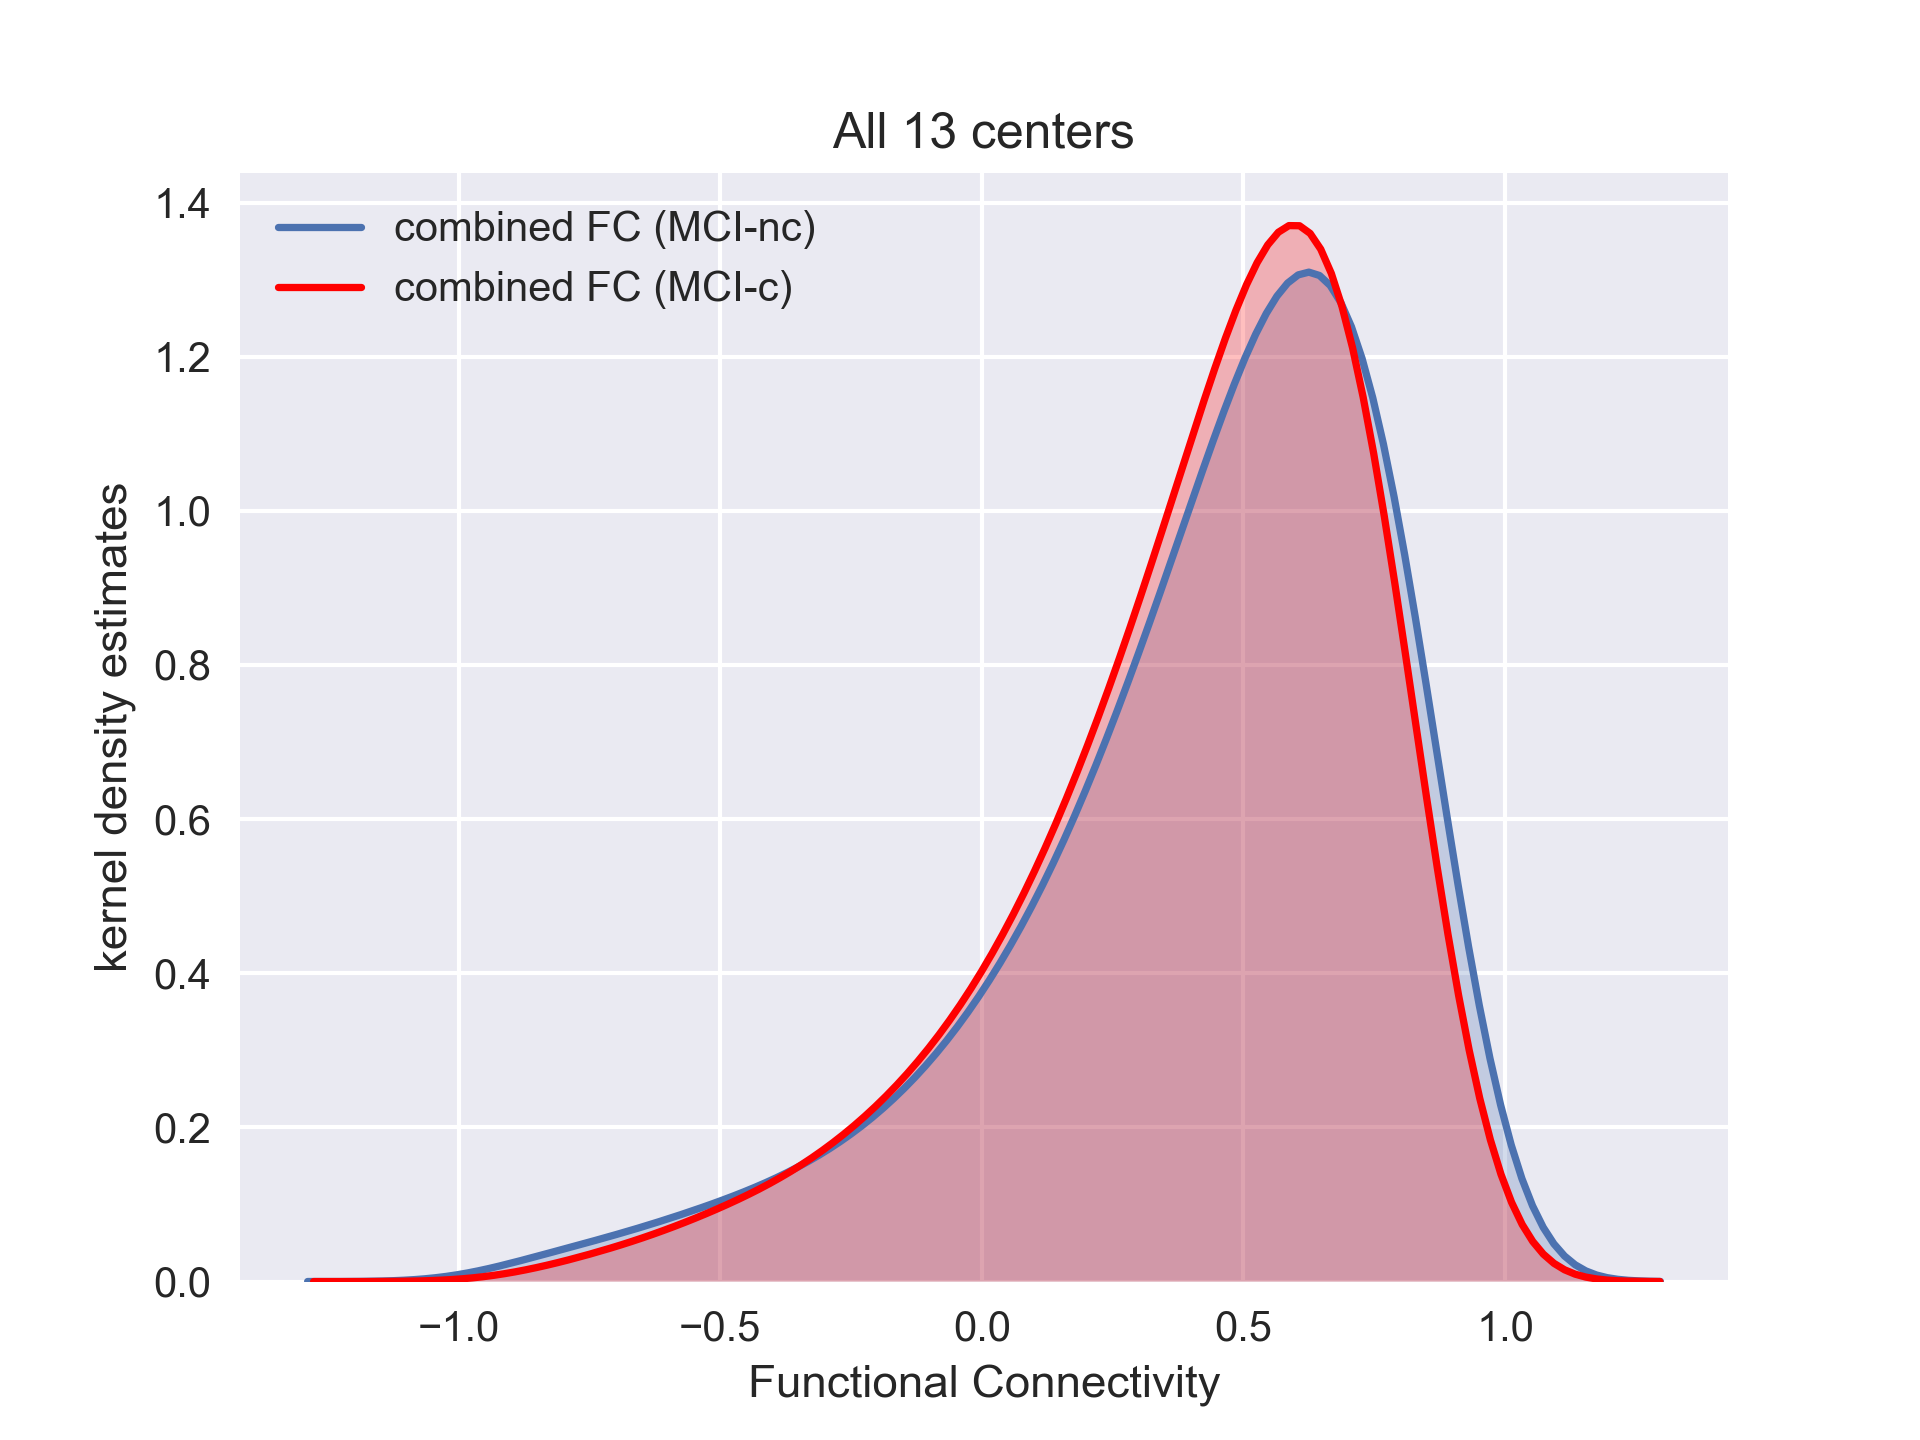
\includegraphics[width=1\linewidth]{fig_distFC_mitjana_TOTS_els_13centres.png}
				%\captionof{figure}{}
				\label{tots_els_centres_FC}
			\end{minipage}%
			\begin{minipage}{.5\textwidth}
				\centering
				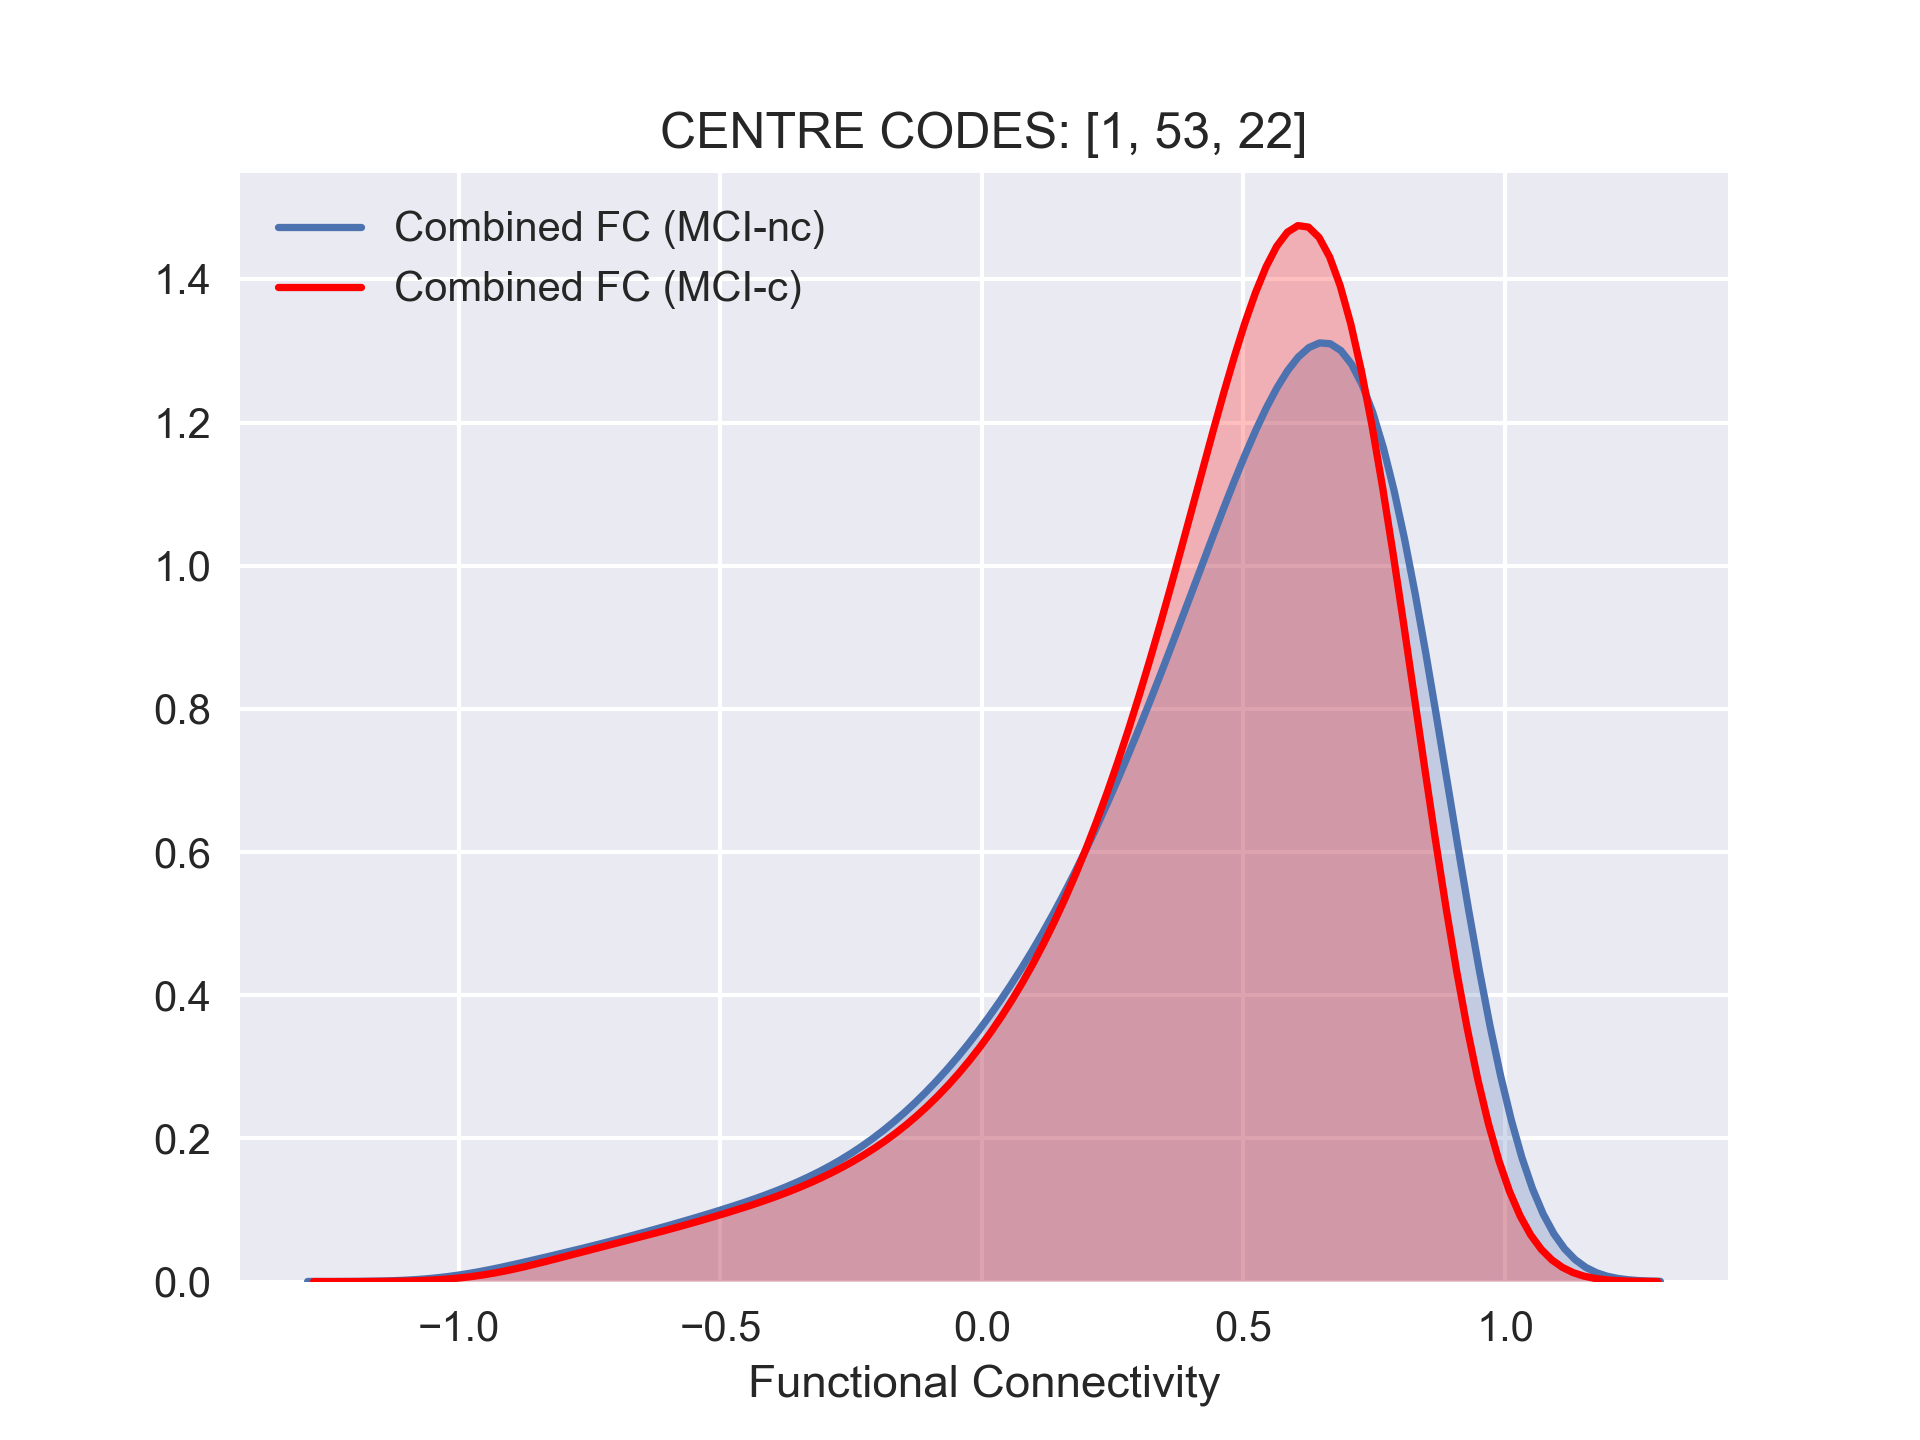
\includegraphics[width=1\linewidth]{fig_distFC_mitjana_centres___1,_53,_22__.png}
				%\captionof{figure}{}
				\label{els3centres_FC}
			\end{minipage}
			\caption{MCI-c vs MCI-nc combined FC distributions for all 13 centres (left image) and the 3 top feeding centers for our sample (right image).}
			\label{FC_dist__tots_els_centres_i_3_top_feeding_centers}
		\end{figure}


		\begin{figure}[h]
		\centering
			%CENTRE 22. 
			\begin{minipage}{.5\textwidth}
				\centering
				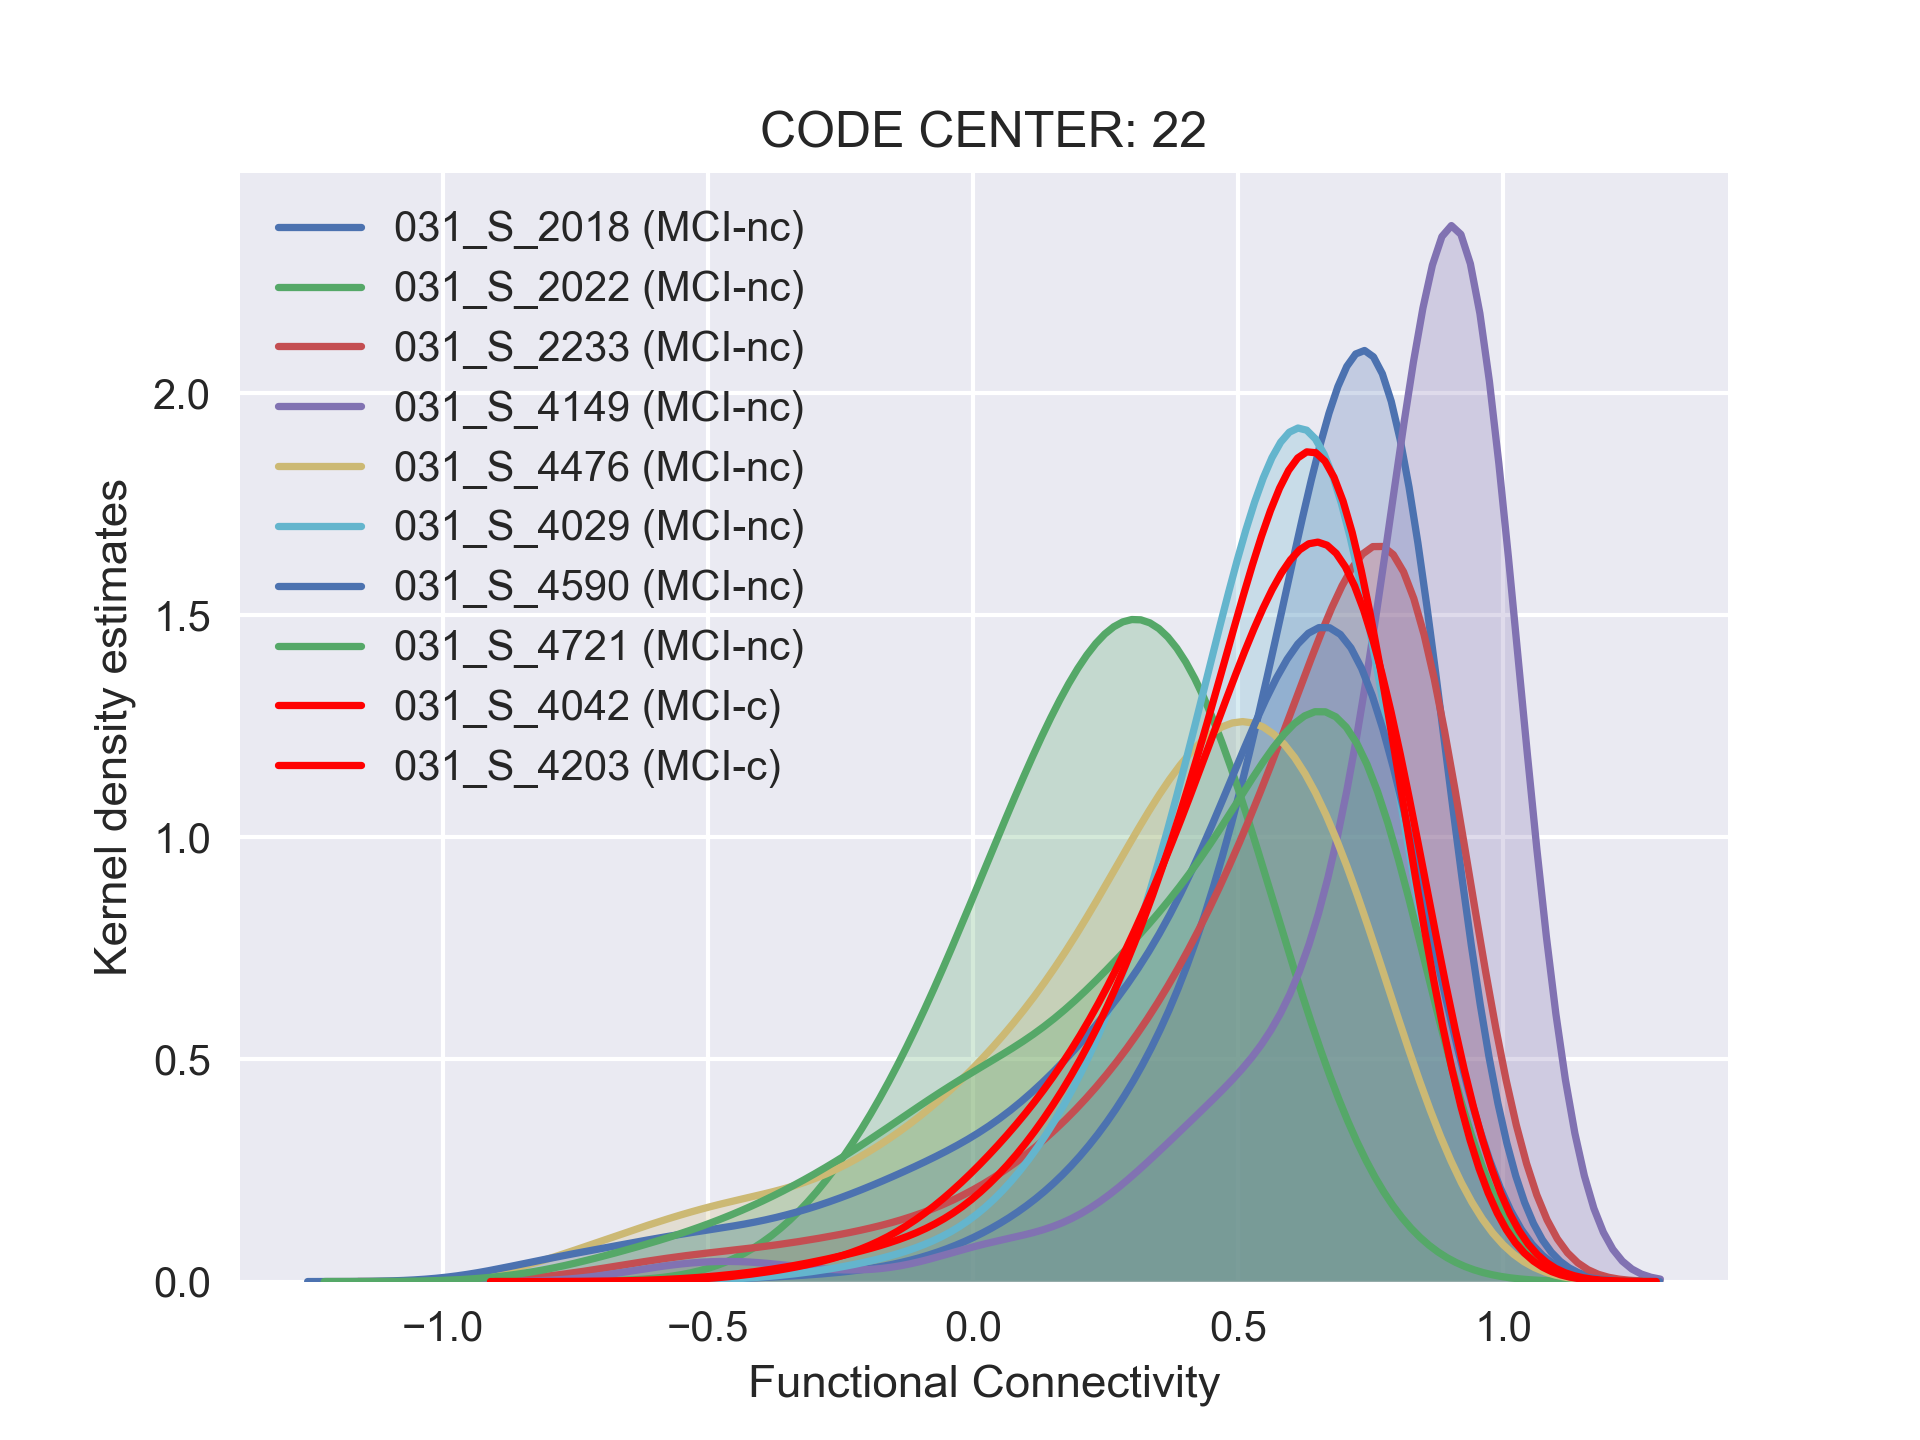
\includegraphics[width=1\linewidth]{fig_distFC_individual_centre_22.png}
				%\captionof{figure}{Multilayer Perceptron confusion matrix.}
				%\label{fig:test1}
			\end{minipage}%
			\begin{minipage}{.5\textwidth}
				\centering
				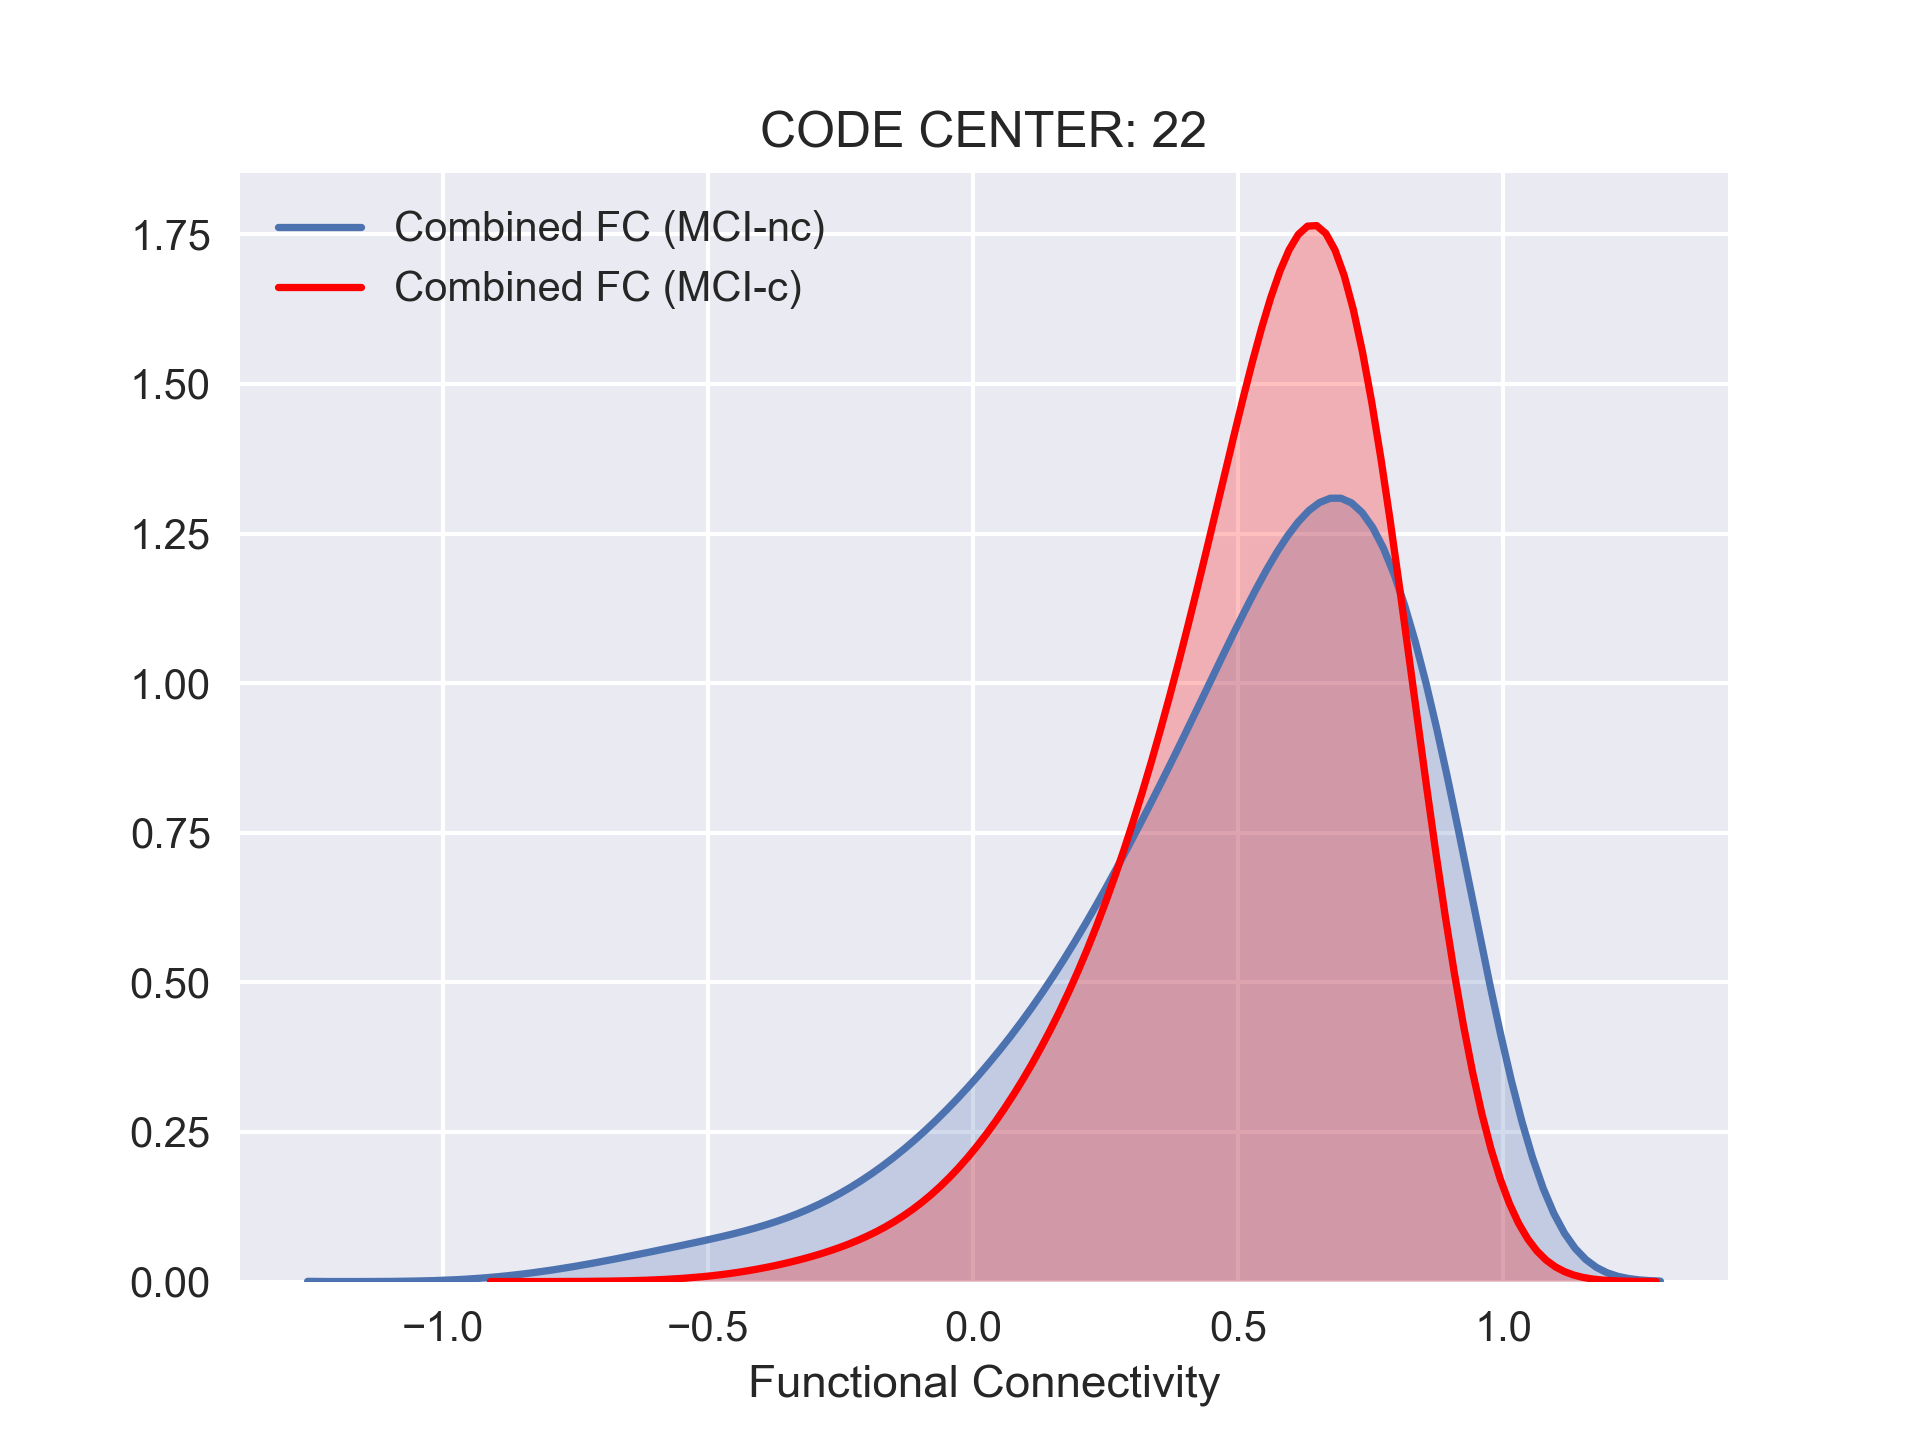
\includegraphics[width=1\linewidth]{fig_distFC_mitjana_centre_22.png}
				%\captionof{figure}{Support Vector machine confusion matrix.}
				%\label{fig:test2}
			\end{minipage}
			%CENTRE 53. 
			\begin{minipage}{.5\textwidth}
				\centering
				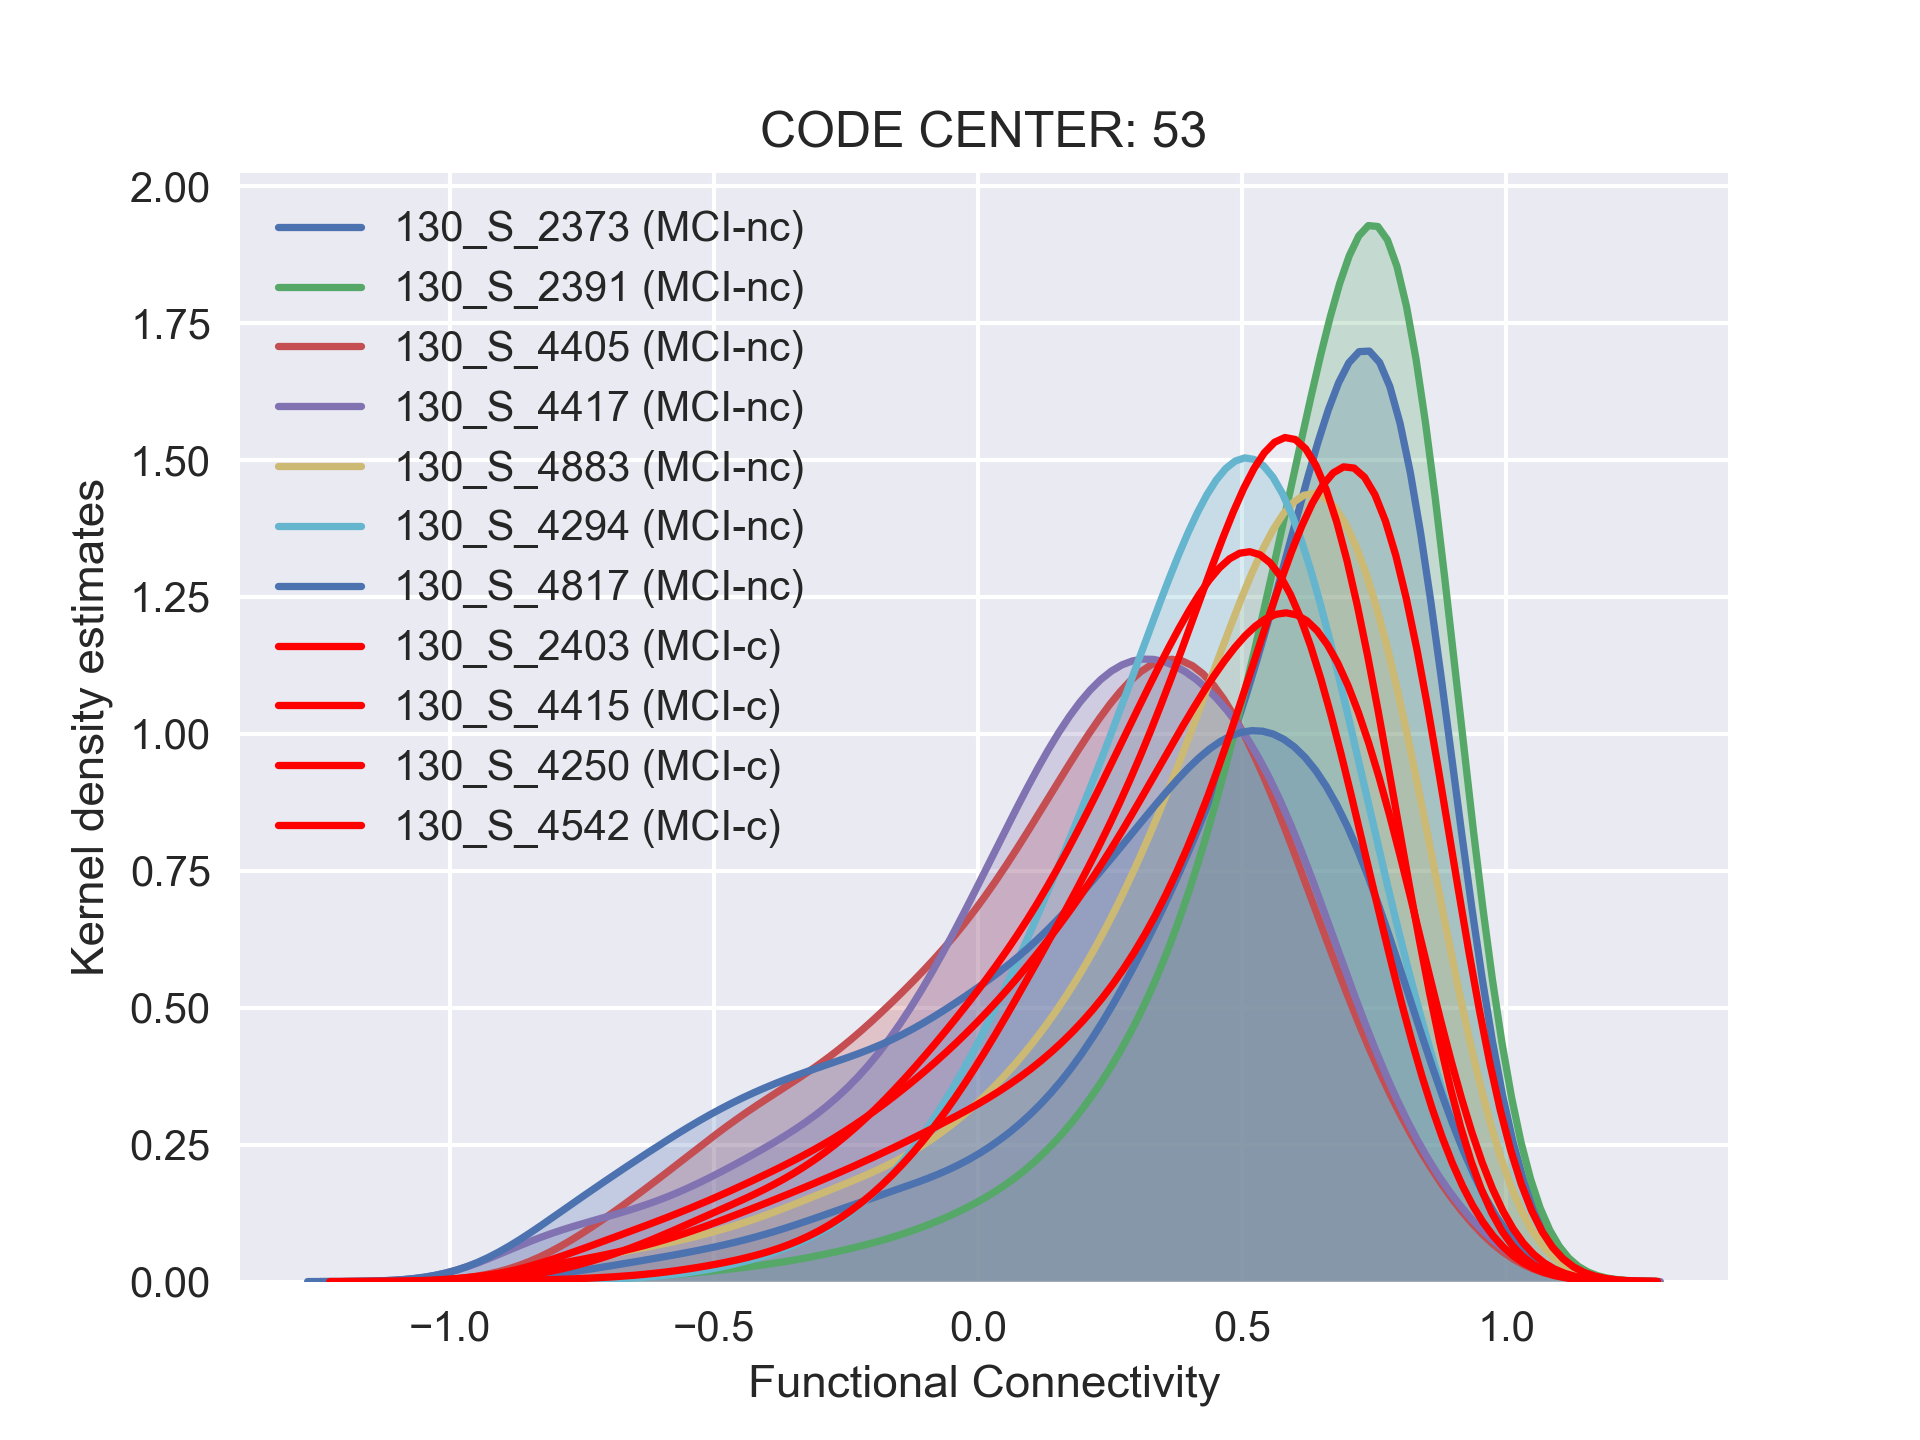
\includegraphics[width=1\linewidth]{fig_distFC_individual_centre_53.png}
				%\captionof{figure}{Multilayer Perceptron confusion matrix.}
				%\label{fig:test1}
			\end{minipage}%
			\begin{minipage}{.5\textwidth}
				\centering
				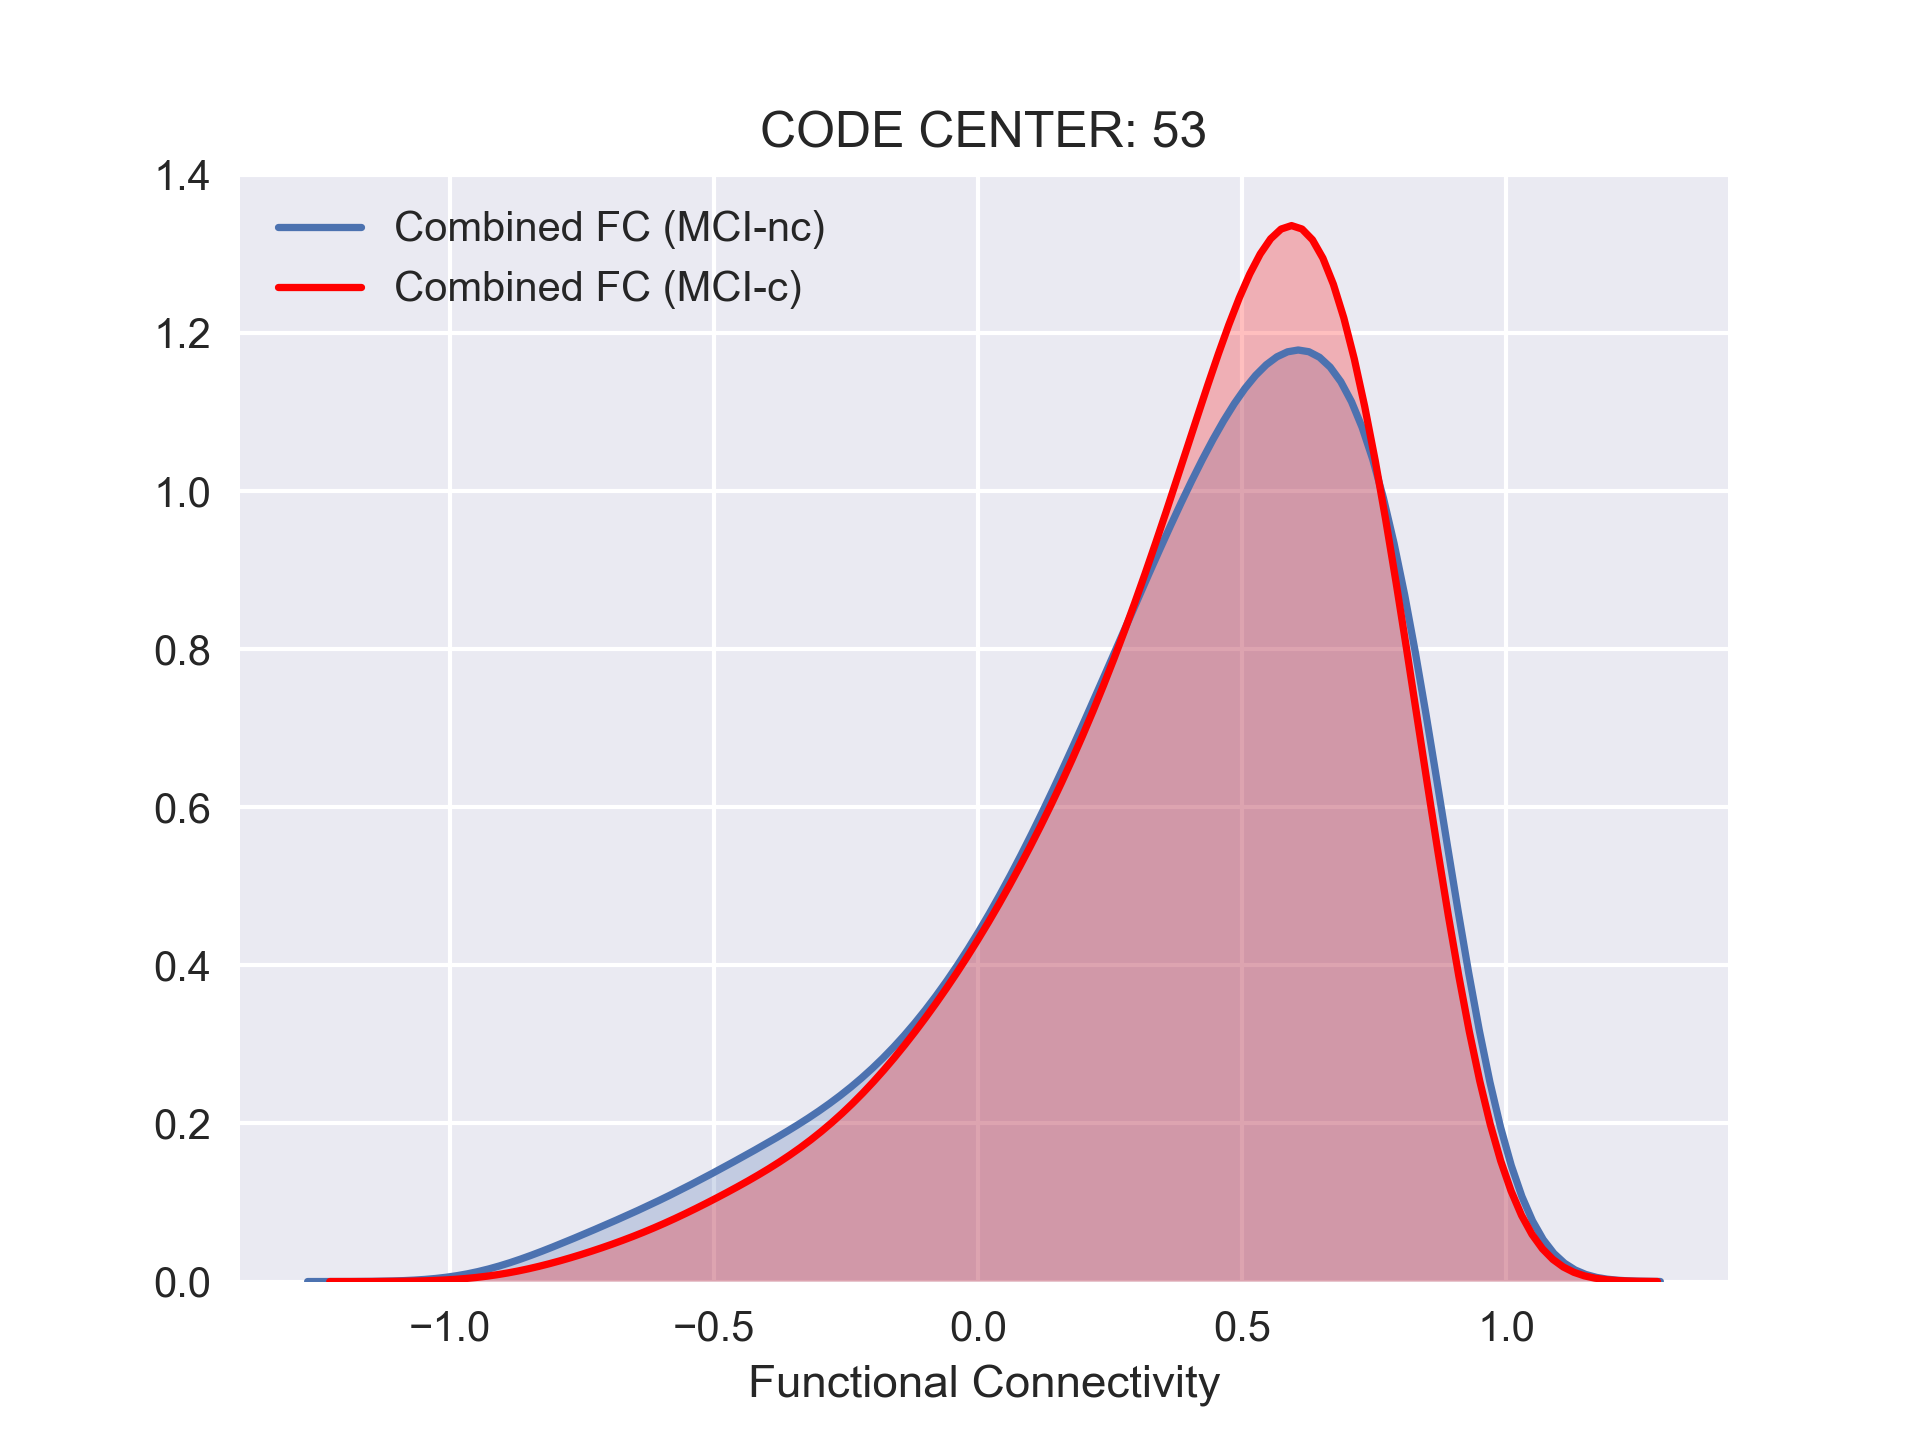
\includegraphics[width=1\linewidth]{fig_distFC_mitjana_centre_53.png}
				%\captionof{figure}{Support Vector machine confusion matrix.}
				%\label{fig:test2}
			\end{minipage}		
			%CENTRE 1. 
			\begin{minipage}{.5\textwidth}
				\centering
				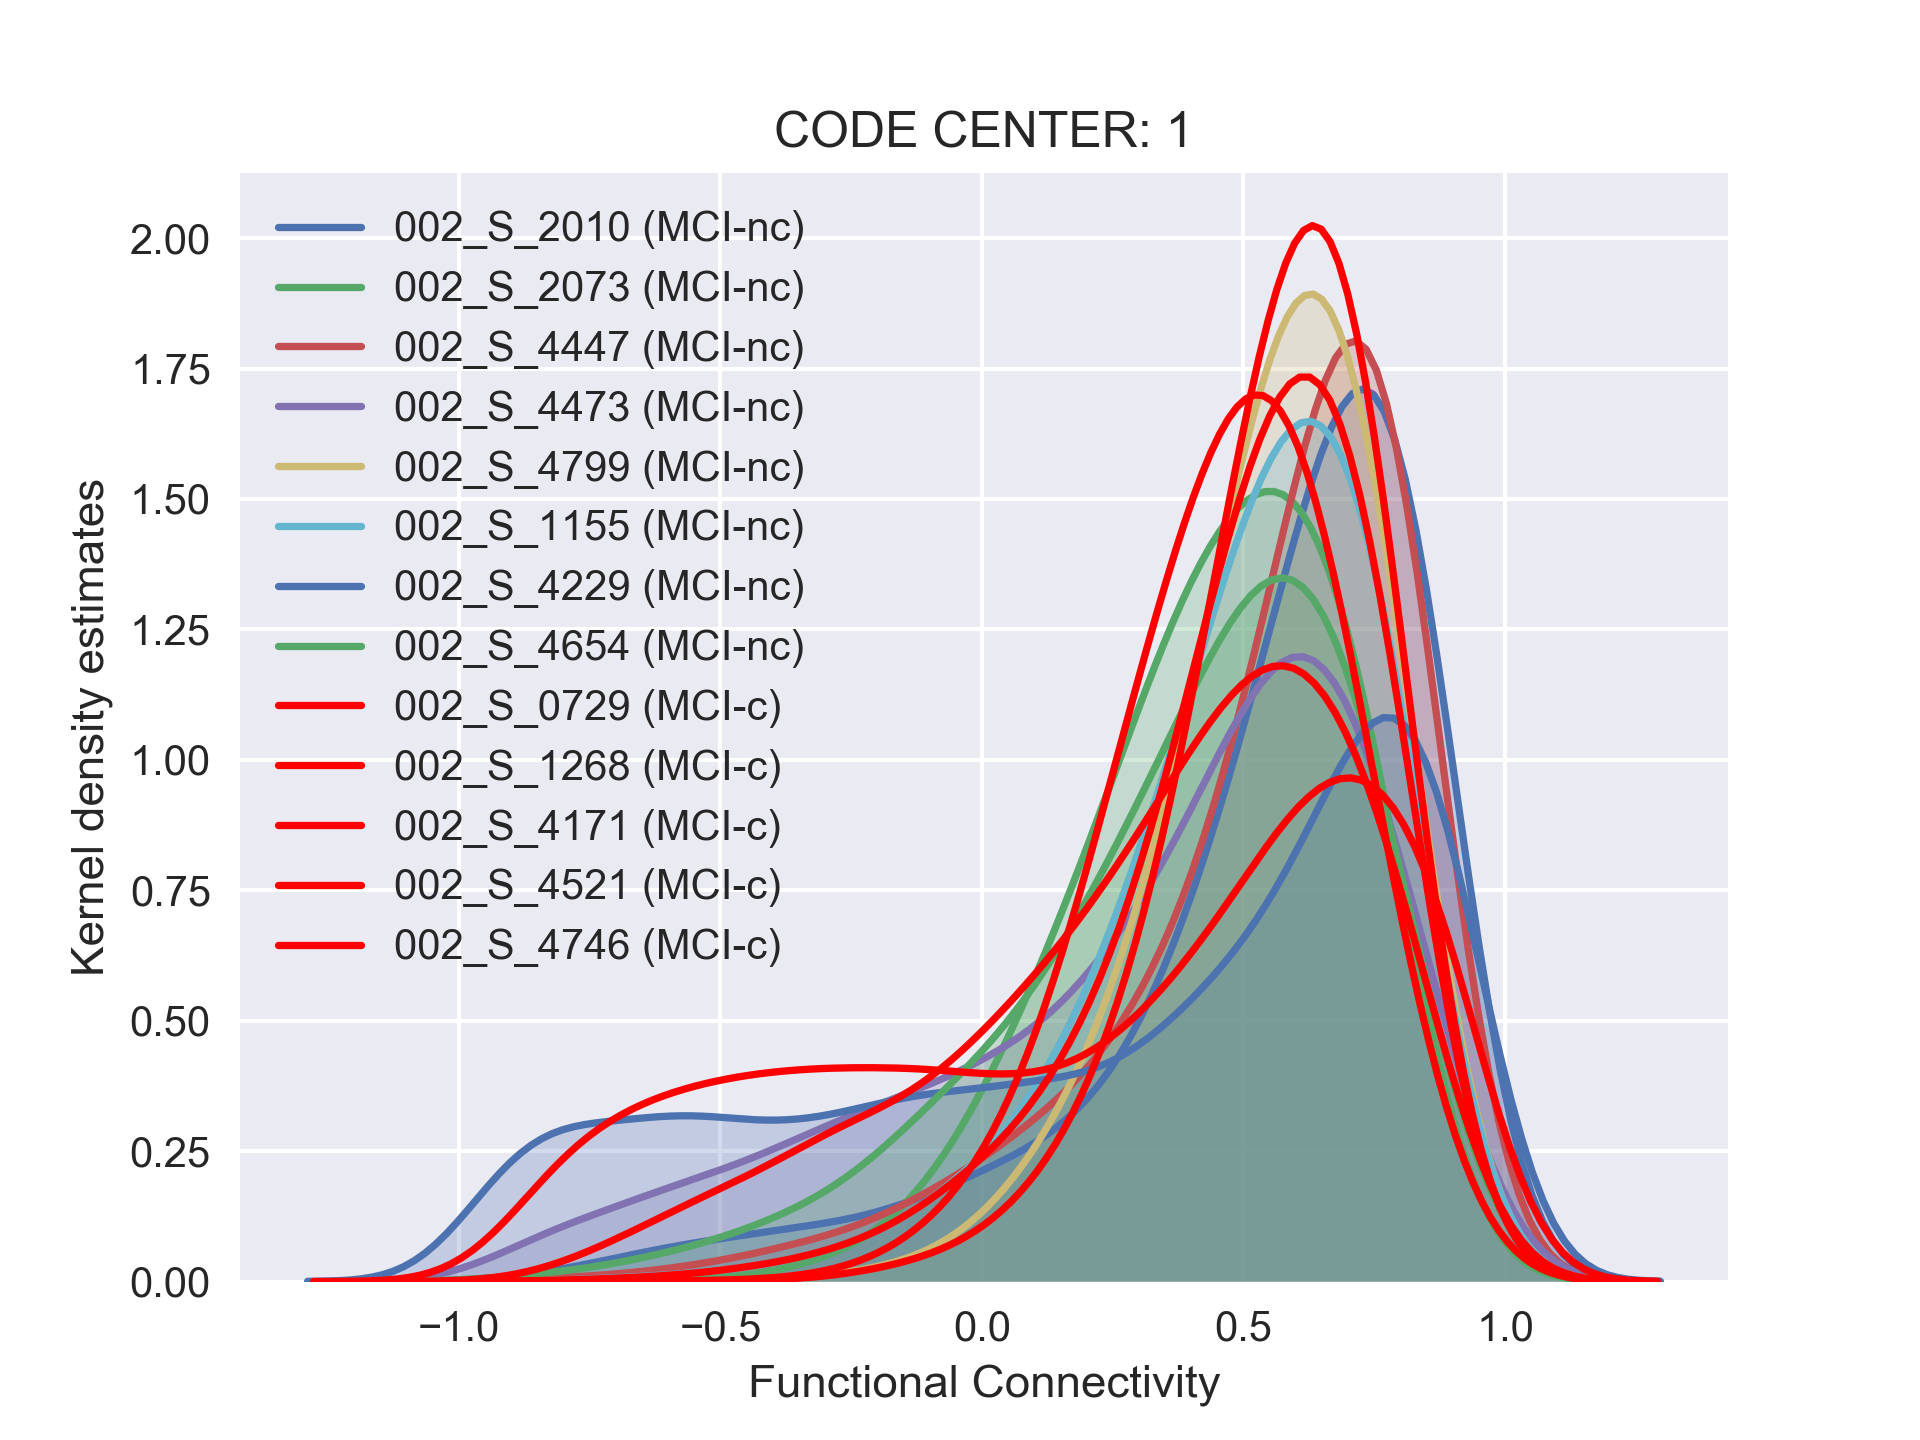
\includegraphics[width=1\linewidth]{fig_distFC_individual_centre_1.png}
				%\captionof{figure}{Multilayer Perceptron confusion matrix.}
				%\label{fig:test1}
			\end{minipage}%
			\begin{minipage}{.5\textwidth}
				\centering
				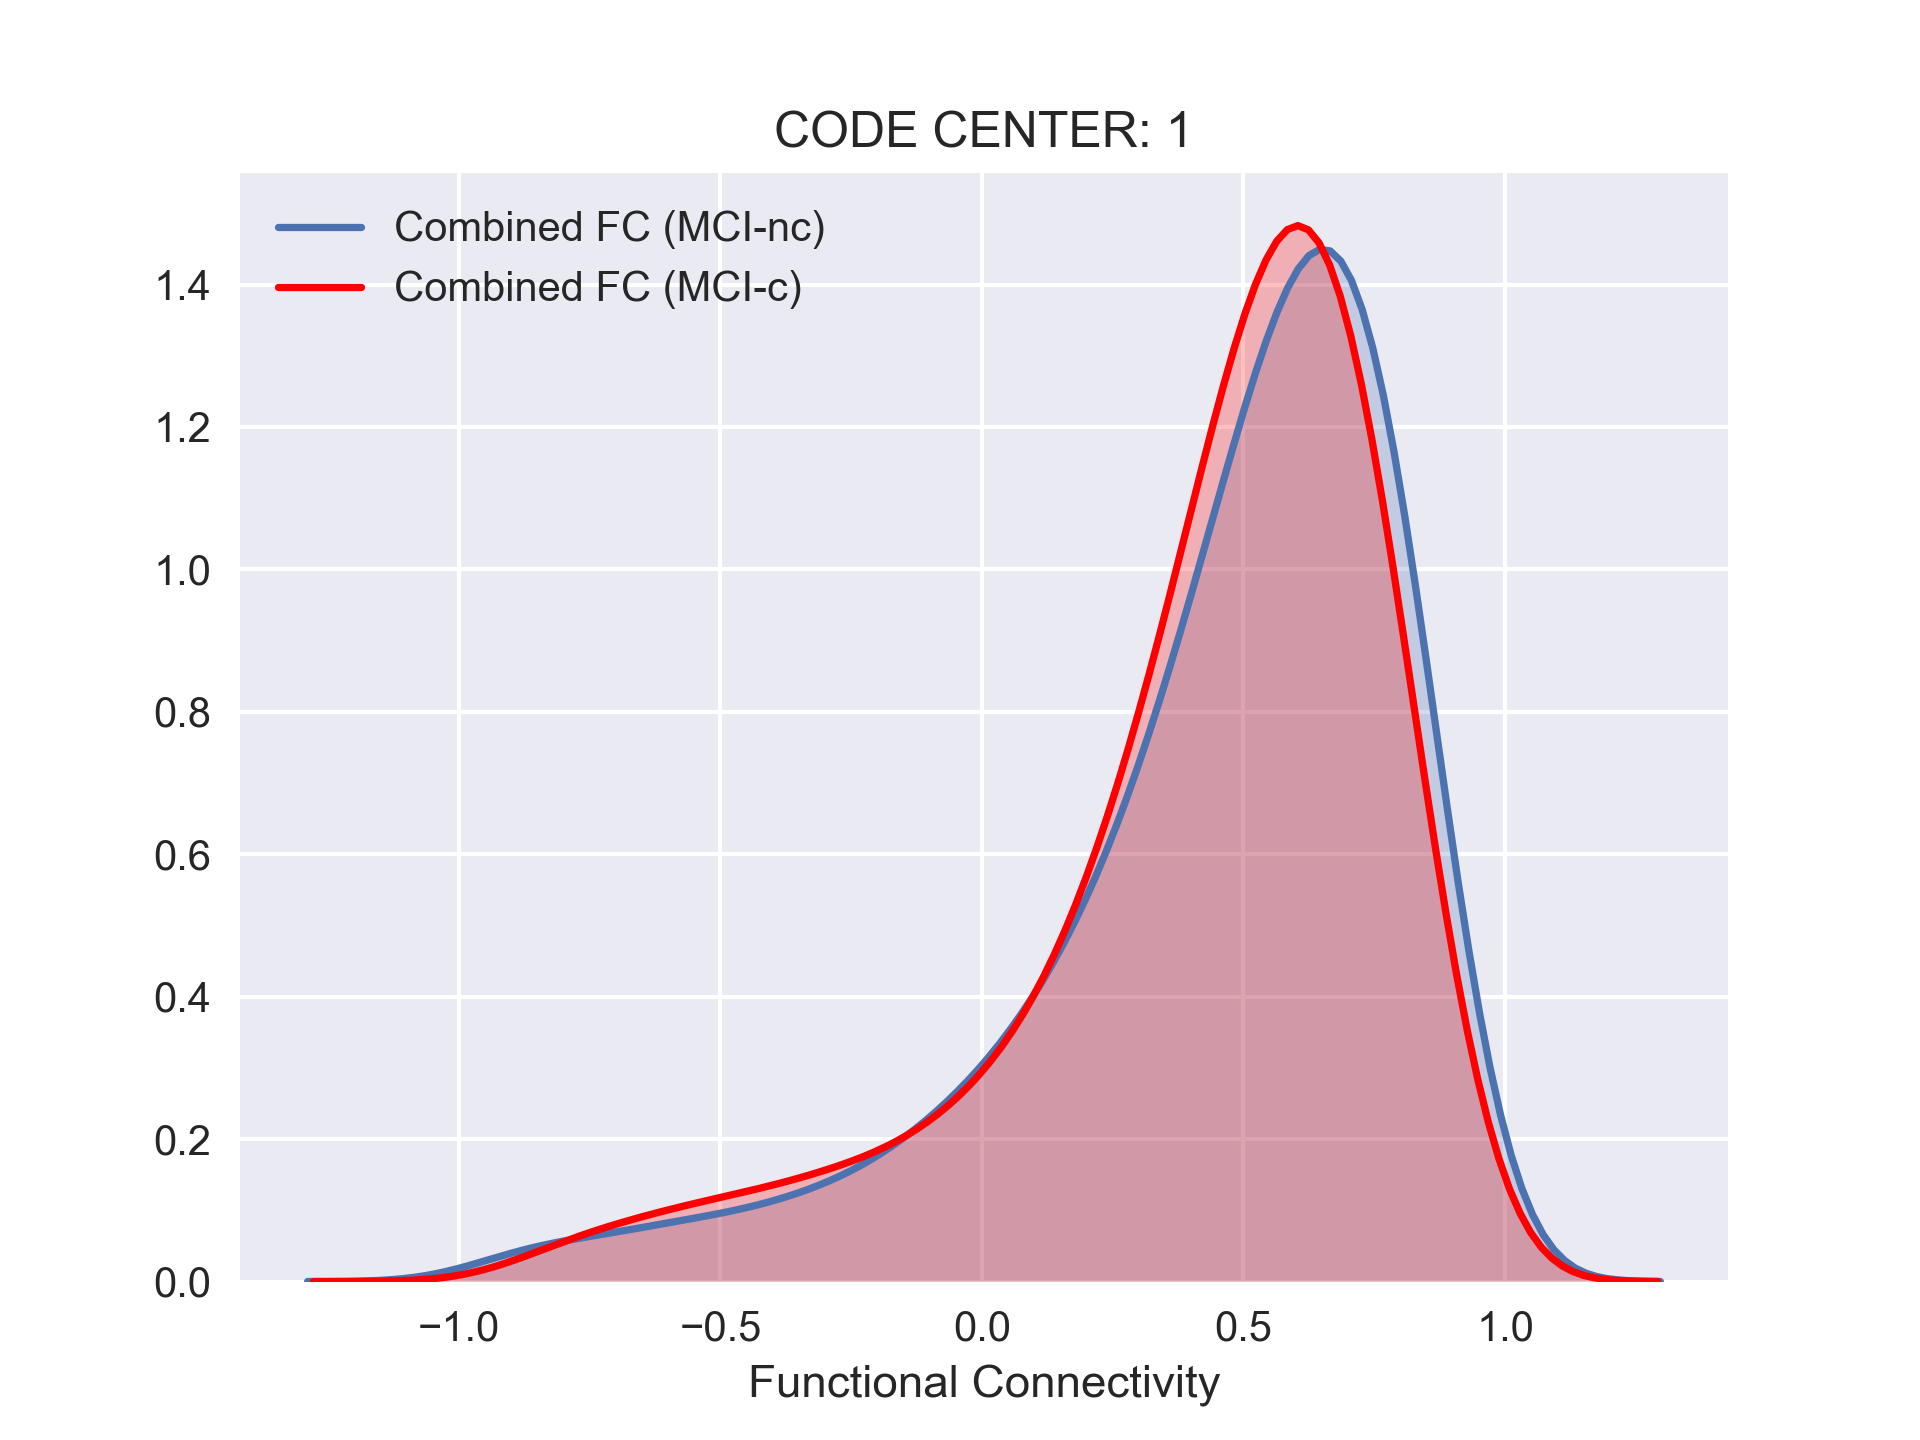
\includegraphics[width=1\linewidth]{fig_distFC_mitjana_centre_1.png}
				%\captionof{figure}{Support Vector machine confusion matrix.}
				%\label{fig:test2}
			\end{minipage}				
					
	
			
		\caption{Kernel density estimates for the three top feeding centers from the ADNI to our sample. In red, distributions for MCI-c participants and in blue for MCI-nc. Left column has distributions at the individual level, whereas the right one has them at grupal level. Mannwhitney tests show very significant test differences among each of the distributions. \textit{NOTE: see homocedasticity and normality assumptions that justify usage of Mann Whitney test in Annex figure \ref{fig:fig_shapiro_levene_FCon}}.}
		\label{fig:FCon_resultats}
	\end{figure}


\FloatBarrier
		
		
		
		
		
		
		
		
		
		

	
		
		
		% AIXO ES AQUI DIR LO DELS CRITERIS INCLUSIO I EXCLUSIO
		% b) TAULA 1: baseline demographic and clinical characteristics of participants    (stard) amb followup time.
		% posar qualitat de neuroimatge aqui potser? en taula potser. mira estudi iranis
		 %c) posar nre participants amb missing data per a predictors. No n'hi ha cap a les matrius.
		%    d) FIGURA: Posa aqui les functional connectivities per grup en matrius d'adjacencia.
	

	
	\FloatBarrier
	\clearpage
	\section{Model metrics}
		\subsection{model diagnostic performances (raw functional connectivity)} 
		% TAULA 2: posa taula accuracy, s, esp, PPV, NPV, LR+, LR- FET
		% TAULA 3: posa taula model fit(brier scores i hosmer-lemeshow)
		% FIGURA: POSAR CURVES ROC
		% FIGURA: comparar les distribucions d'accuracies per fold entre models, d'acord amb el proposat per andrea. FET
		\begin{table}[h]
		\centering
			\begin{threeparttable}
				\caption{Diagnostic accuracy metrics per model after the cross-validation (\textit{Functional connectivity} as predictors, and no dimensionality reduction)}
				\label{table:taula_diagnostic_metrics_fMRI_nodimreduc}
				\begin{tabular}{lllllllll}	
					\toprule
					classifier&acc$^{i}$&sen$^{i}$&spec$^{i}$&PPV$^{i}$&NPV$^{i}$&LR+&LR-&AUC$^{ii}$\\
					\midrule
					
					MLP$^{a}$ & 77.03 & 47.83 & 90.20 & 68.75 & 79.31 & 4.878 & 0.578 & 0.81\\
					LR$^{b}$ & 75.68 & 47.83 & 88.24 & 64.71 & 78.95 & 4.065 & 0.591 & 0.75\\
					SVM$^{c}$ & 75.68 & 39.13 & 92.16 & 69.23 & 77.05 & 4.989 & 0.660& 0.82\\
					NN$^{d}$ & 66.22 & 26.09 & 84.31 & 42.86 & 71.67 & 1.663 & 0.877 & 0.57\\
					GNB$^{e}$ & 60.81 & 26.09 & 76.47 & 33.33 & 69.64 & 1.109 & 0.967 & 0.63\\
					\bottomrule
				\end{tabular}
				\begin{tablenotes}
					\tiny\item[]{\textit{$^{ii}$ Area under the ROC curve} $|$ \textit{$^{i}$Expressed in \% $||$}$^{a}$Multilayer perceptron (Artificial Neural Network) $|$ $^{b}$Logistic Regression $|$ $^{c}$Support Vector Machines (linear kernel)$|$ $^{d}$Nearest Neighbours $|$$^{e}$Gaussian Naive Bayes}
				\end{tablenotes}

			\end{threeparttable}
		\end{table}
		
		\FloatBarrier
		
		
		A complete list of all the in-sample accuracy metrics obtained \textit{after} the 10-fold cross-validation for all 5 machine learning models can be directly consulted in table \ref{table:taula_diagnostic_metrics_fMRI_nodimreduc}. You can consult MLP, SVM and LR confusion matrices in figure \ref{fig:bestperformingmodels_CONFUSIONS}, and ROC curves and AUC estimates by cross-validation fold in figure \ref{fig:MLPiSVM_ROCs} for the former two and figure \ref{fig:LR_ROC} for the latter.

		
		First off, there are two models that have performed poorely: Nearest Neighbours and Gaussian Naive Bayes. These models have shown the worst accuracy metrics and, thus, their ROC curves and confusion matrices are not even reported in the results section (they are reported in the annex section \ref{sec:fig_NaiveBayes_fMRI_nodimreduc_CONFUSIONiROCCURVE} instead, and this is the only paragraph we will comment upon them). Both of them show positive likelihood ratios very close to 1\footnote{Above 1, $LR+$ is better the higher it is. A perfect $LR+$ would tend to infinity, that is very high sensitivity and very high specificity.}($LR+_{NN} = 1.666$, $LR+_{GNB} = 1.109$) which means that, in our sample, when these models have diagnosed patients as MCI converters or MCI-c (i.e, with positive test results) they were actually as likely to have an AD onset than just remaining having MCI. Hence, they are absolutely useless to give any predictive value: they cannot forecast if someone will turn to AD. For these two models, confidence with negative test results is also poor, since they also show $LR-$ values not far below 1\footnote{A negative likelihood ratio is better the smaller it is. When close to 0, means that is very unlikely that a diseased person (MCI-c) is missed by the test and also that is very likely that a `healthy' one (MCI-nc) is diagnosed as healthy.} ($LR-_{NN} = 0.877$, $LR-_{GNB} = 0.967$), which means confidence in negative test results (that is if the model categorizes someone as MCI-nc) is close to random.  
		
		Finally brier Scores per model are 0.230 for the MLP, 0.243 for both LR and SVM, 0.338 for NN and 0.392 for GNB. As you can see here these measures assess not only model calibration but also model performance (since MLP, LR, SVM have very comparable performances, yet not all of them exhibit the same default calibrations).






		
		%VIOLIN PLOTS 
		\begin{figure}[h]
			\centering
			\begin{subfigure}[a]{1\textwidth}
				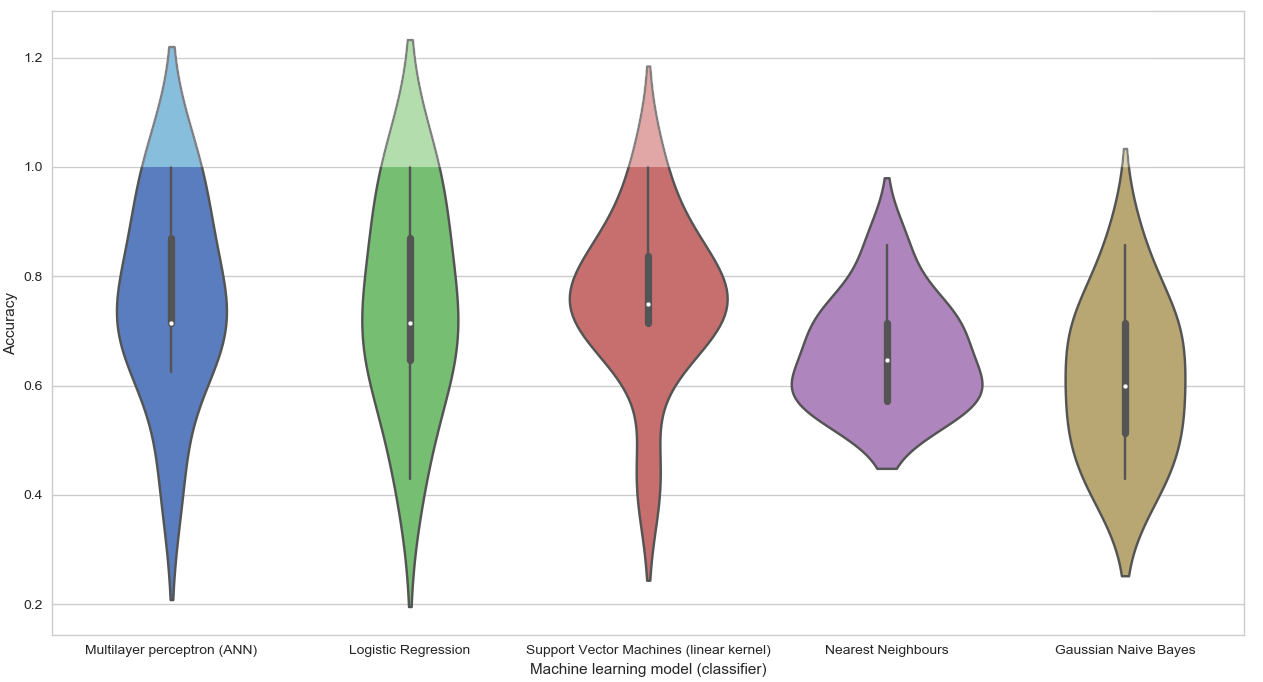
\includegraphics[width=1\textwidth]{fig_comparacio_models_fMRI_nodimreduc_ACCURACYPLOT.png}
				\caption{Accuracy distributions. Support vector machine performs slightly -although not significantly better- than the rest.}
				\label{fig_comparacio_models_fMRI_nodimreduc_ACCURACYPLOT} 
			\end{subfigure}
			\begin{subfigure}[b]{1\textwidth}
				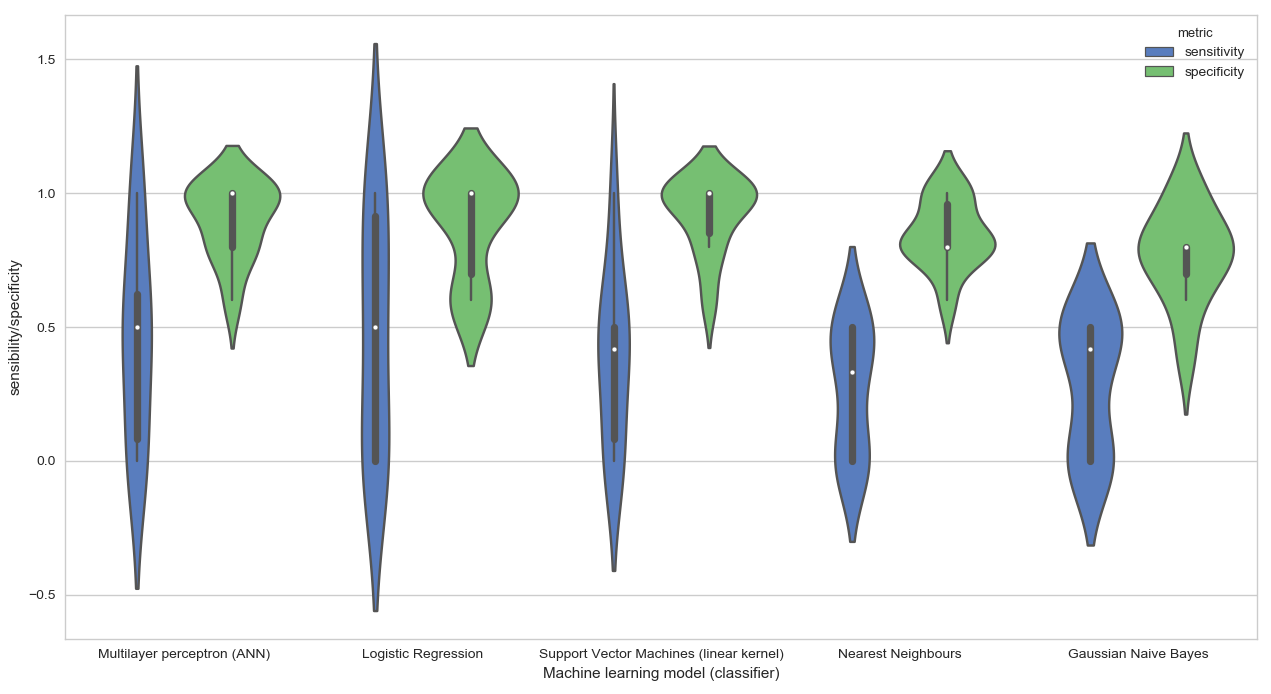
\includegraphics[width=1\textwidth]{fig_comparacio_models_fMRI_nodimreduc_SENSIBILITATESPECIFICITAT.png}
				\caption{Sensitivity and specificity distributions. Best balance between both metrics has been achieved by Logistic regression and Multilayer Perceptron.}
				\label{fig_comparacio_models_fMRI_nodimreduc_SENSIBILITATESPECIFICITAT}
			\end{subfigure}
			
			\caption{Violin plots$^{**}$ for the distributions of three diagnostic metrics: accuracy, sensitivity and specificity, for each of the 5 machine learning models. Each distribution is composed by 10 values for a given metric (each of those are obtained in each test split -one per each fold- of the 10-fold cross-validation). For these models, the predictors used as input matrix are the raw vectorized \textbf{functional connectivities} -no dimensionality reduction or feature selection-. $||$ $^{**}$\textit{The violin plot shows medians for the distributions as white dots. IQR or Interquartile range, similar to a boxplot, is shown with the black box. 95\% confidence intervals out of the cross-validation are depicted as black wide lines in the graph-}.}
		\end{figure}
		\clearpage	
		
		%MATRIUS DE CONFUSIO PER ALS 3 MILLORS MODELS DE FMRI
	
			\begin{figure}[h]
			\centering
			\begin{minipage}{.33\textwidth}
				\centering
				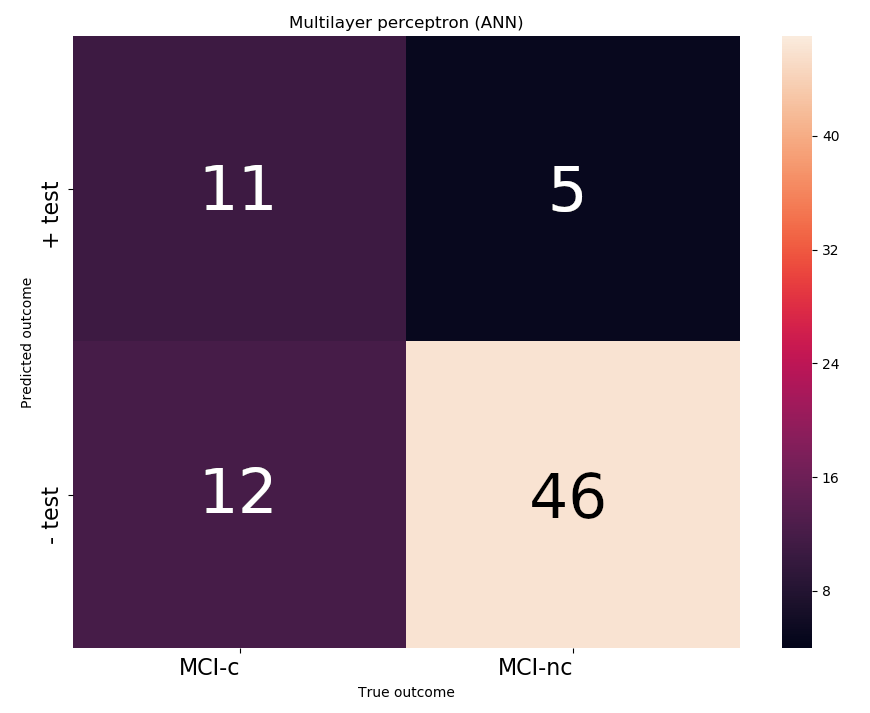
\includegraphics[width=1\linewidth]{fig_MLP_fMRI_nodimreduc_CONFUSION.png}
				%\captionof{figure}{Multilayer Perceptron confusion matrix.}
				%\label{fig:test1}
			\end{minipage}%
			\begin{minipage}{.33\textwidth}
				\centering
				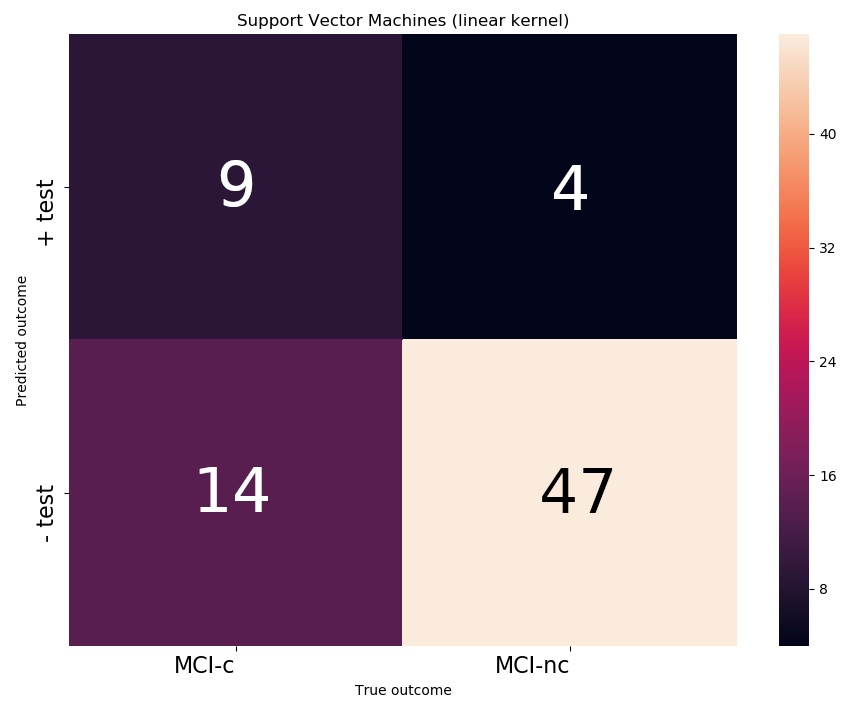
\includegraphics[width=1\linewidth]{fig_SVM_fMRI_nodimreduc_CONFUSION.png}
				%\captionof{figure}{Support Vector machine confusion matrix.}
				%\label{fig:test2}
			\end{minipage}
			\begin{minipage}{.33\textwidth}
				\centering
				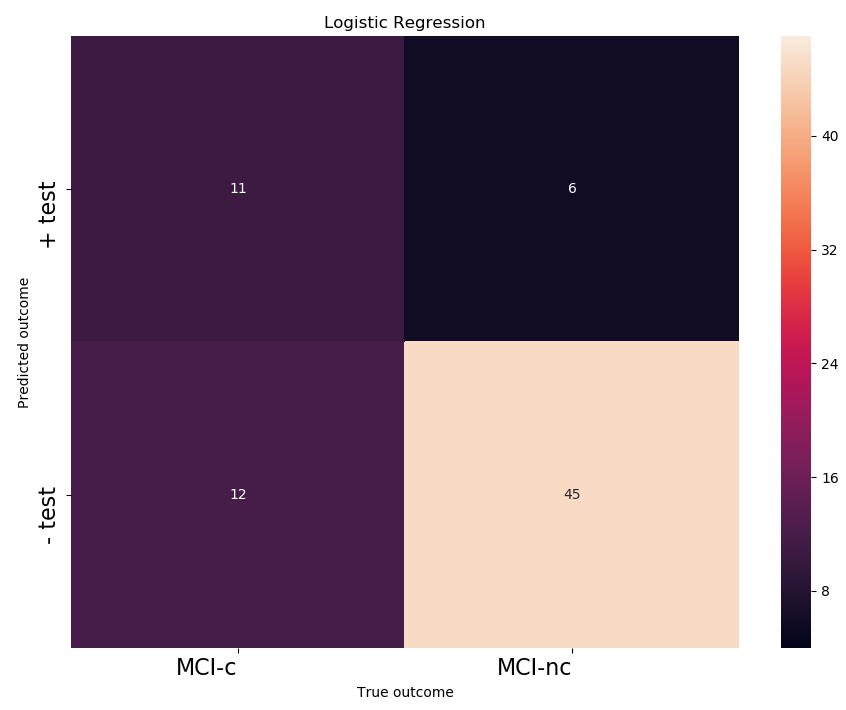
\includegraphics[width=1\linewidth]{fig_LR_fMRI_nodimreduc_CONFUSION.png}
				%\captionof{figure}{Logistic Regression confusion matrix.}
				%\label{fig:test2}
			\end{minipage}
			\caption{Heat map of the confusion matrices obtained after the sum of the TP,TN,FP and FN across all folds of the cross-validation, for each of 3 types of models. From left to right Multilayer Perceptron, Support Vector Machines and Logistic Regression. This is where the data in table \ref{table:taula_diagnostic_metrics_fMRI_nodimreduc} comes from. \textit{NOTE: GNV and NN classifiers confusion matrices are depicted in Annex, section \ref{sec:fig_NaiveBayes_fMRI_nodimreduc_CONFUSIONiROCCURVE}}.}
			\label{fig:bestperformingmodels_CONFUSIONS}
		\end{figure}
		\FloatBarrier
		
		
		
		
		
		Positive likelihood ratios are around 4 or 5 for Multilayer perceptron (MLP), Logistic regression (LR) and Support vector machines (SVM), and negative likelihood ratios are around 0.5 or 0.6 which means they obtain a better predictive accuracy. The highest diagnostic accuracy in our sample has been achieved by the multilayer perceptron ($Acc_{MLP}$ = 77.03\%, 95\% CI from 67 to 87\%), followed at the same distance by Logistic regression and Support Vector Machines ($Acc_{LR}$ = $Acc_{SVM}$ = 75.68\%, 95\% CI from 66 to 85\%)	\footnote{These confidence intervals are built considering this estimates simple proportions, and considering sample size to be all the development set. Figures \ref{fig_comparacio_models_fMRI_nodimreduc_SENSIBILITATESPECIFICITAT} and \ref{fig_comparacio_models_fMRI_nodimreduc_ACCURACYPLOT}}. In terms of accuracy, we cannot say one model is better than the other at population level, since all the confidence intervals of these estimates overlap. However, all these three models show accuracies above average level (i.e. they allow us to reject the null hypothesis that has 50\% accuracy\footnote{(1/k)*100, where k is number of classes or categories -in this case, two-.} as its decision boundary). The only model that does not allow to reject the null hypothesis is the Gaussian Naive Bayes ($Acc_{MLP}$ = 60.81\%, 95\% CI from 50 to 72\%), since has a slightly overlapping confidence interval over decision threshold. You can consult the distribution of accuracies per classifier across the 10 folds of the cross-validation in figure \ref{fig_comparacio_models_fMRI_nodimreduc_ACCURACYPLOT}.
	



		



		
		It is worth noting that SVM, MLP and LR have shown very high specificities ($spec_{SVM}$ = 92.16, 95\% CI from 86 to 98\%; $spec_{MLP}$ = 90.20, 95\% CI from 83 to 97\%; $spec_{LR}$ = 88.24, 95\% CI from 81 to 96\%)\footnote{These confidence intervals are built considering this estimates simple proportions, and considering sample size to be all our sample, not the test size of a train/test split. Figures \ref{fig_comparacio_models_fMRI_nodimreduc_SENSIBILITATESPECIFICITAT} and \ref{fig_comparacio_models_fMRI_nodimreduc_ACCURACYPLOT}  also show 95\% Confidence intervals -slimest black lines-, but those are built upon the distribution of diagnostic accuracy metrics from the cross-validation, not around the classical proportion intervals, so they might depict some differences to the ones reported here.} and at the same time very low sensitivities ($sen_{SVM}$ = 39.13, 95\% CI from 28 to 50\%; $sen_{MLP}$ = 47.83, 95\% CI from 36 to 59\%; $sen_{LR}$ = 47.83, 95\% CI from 36 to 59\%). You can see sensitivity and specificity estimates in the violin plots for figure \ref{fig_comparacio_models_fMRI_nodimreduc_SENSIBILITATESPECIFICITAT}.
		


				%CURVES ROC DE SVM I MLP
				\begin{figure}[t]
				\centering
				\begin{minipage}{.5\textwidth}
					\centering
					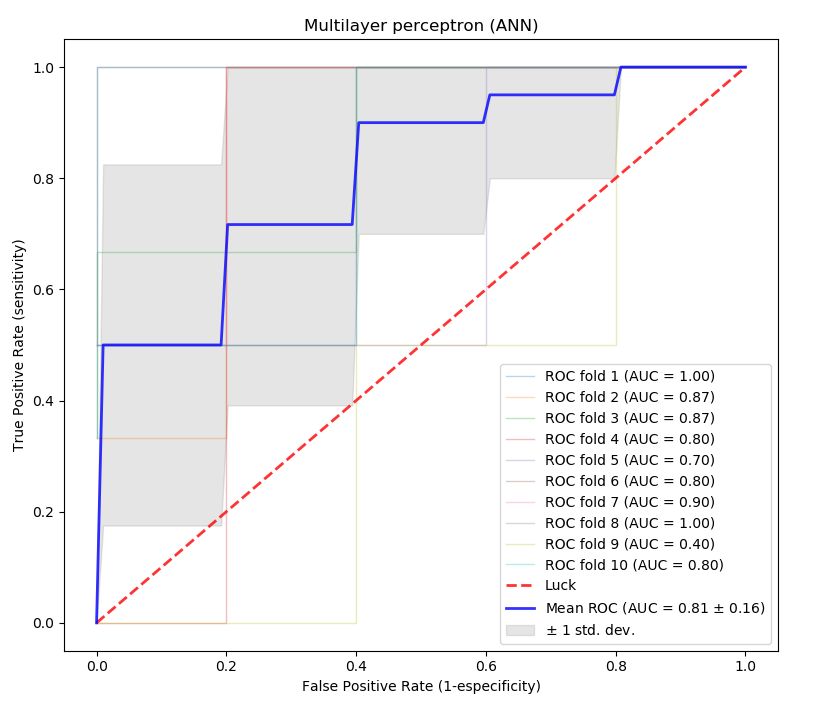
\includegraphics[width=1\linewidth]{fig_MLP_fMRI_nodimreduc_ROC.png}
					%\captionof{figure}{Multilayer Perceptron confusion matrix.}
					%\label{fig:test1}
				\end{minipage}%
				\begin{minipage}{.5\textwidth}
					\centering
					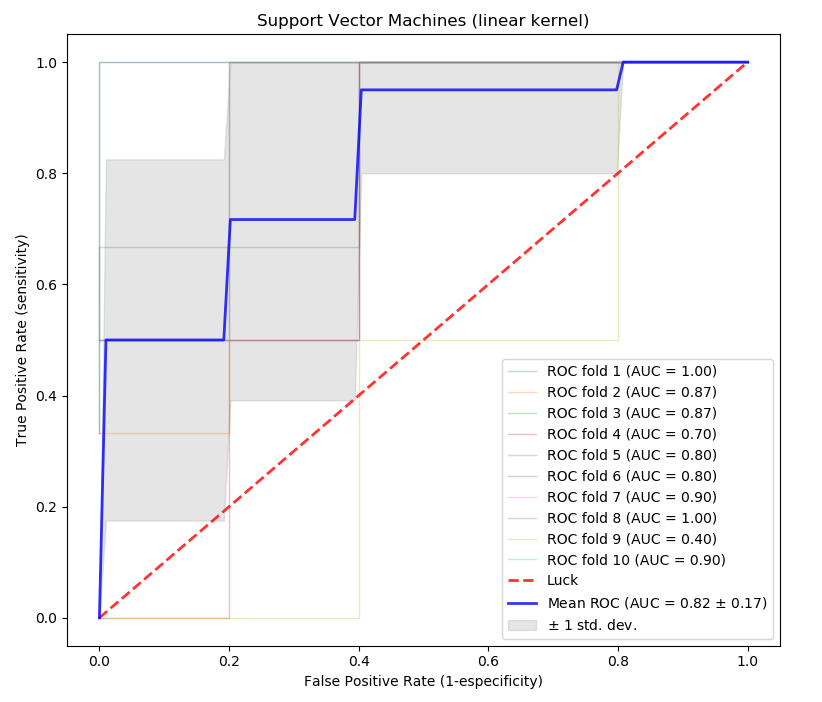
\includegraphics[width=1\linewidth]{fig_SVM_fMRI_nodimreduc_ROC.png}
					%\captionof{figure}{Support Vector machine confusion matrix.}
					%\label{fig:test2}
				\end{minipage}
				\caption{ROC curves for the SVM and LR for raw \textit{functional connectivities} as precdictors, with mean AUCs of 0.81 and and 0.82 AUC, respectively. You can see a ROC curve for each fold of the cross-validation -weaker lines- the mean ROC curve -blue line- and also the corresponding AUC for each roc curve in the legend. final Mean roc curve is `wrapped' by plus minus the standard deviation.}
				\label{fig:MLPiSVM_ROCs}
			\end{figure}

			%CURVA ROC DE LR
			\begin{wrapfigure}{l}{0.5\textwidth}
				\begin{center}
					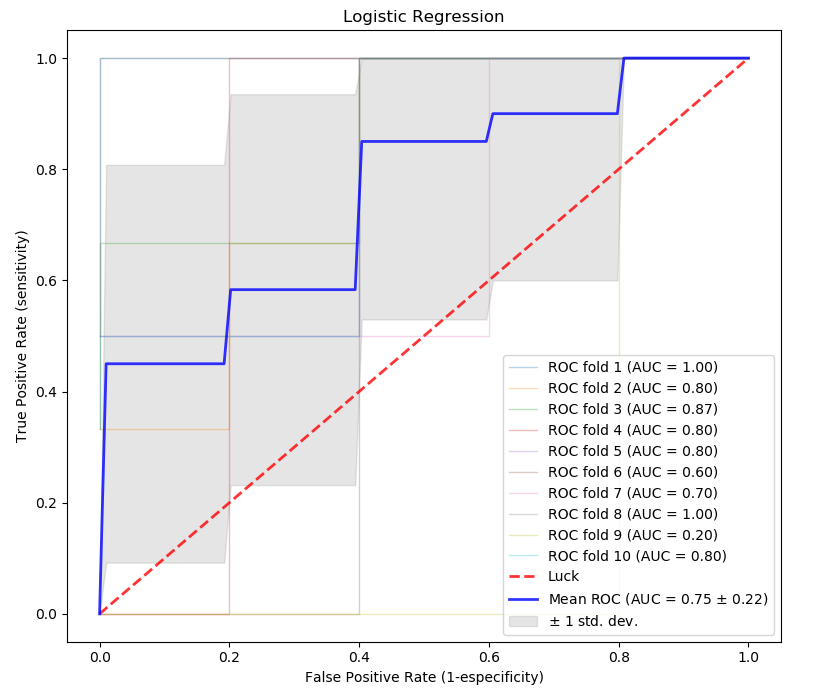
\includegraphics[width=0.48\textwidth]{fig_LR_fMRI_nodimreduc_ROC.png}
				\end{center}
				\caption{ROC curve for the LR model for raw \textit{functional connectivities} as predictors. AUC = 0.75}
				\label{fig:LR_ROC}
			\end{wrapfigure}

The MLP, LR and SVM show precisions around 75 to 80\%, all of them above chance level ($PPV_{MLP}$ = 68.75, 95\% CI from 58 to 79\%; $PPV_{LR}$ = 64.71, 95\% CI from 54 to 76\%; $PPV_{SVM}$ = 69.23 , 95\% CI from 59 to 80\%). Similarly, in our sample, the probability that a negative diagnostic (MCI-nc) is correct goes from 77 to 79\% depending on the model ($NPV_{MLP}$ = 79.31, 95\% CI from 70 to 89\%, $NPV_{LR}$ = 78.95, 95\% CI from 80 to 88\%, $NPV_{SVM}$ = 77.05, 95\% CI from 67 to 87\%).		
	\FloatBarrier

	
\hfill \hfill \break \break Finally AUCs for MLP, SVM and LR are 0.81 ($\pm$ 0.16), 0.82 ($\pm$ 0.17) and 0.75 ($\pm$0.22). Confidence intervals, in this case, do not `wrap' the estimates: standard deviations are displayed instead. You can consult figure \ref{fig:MLPiSVM_ROCs} and figure \ref{fig:LR_ROC} to access to ROC curve and AUC estimates per fold.


		\subsection{model diagnostic performances (functional connectivity with dimensionality reduction)}
		
		The models with dimensionality reduction of functional connectivity had poor results (0\% specificity). Thus, no reporting is made (you can see a discussion in \ref{sec:unexpected}).
		
		\subsection{multimodal approach with biomarkers, questionnaires and functional connectivity}
	
		Hypothesis \textit{\textbf{H2}} (see \ref{study_objectives}) was not completely met, since all fMRI models had low sensitivities). Thus, we did not attempt a multimodal approach.
		
		

		\subsection{model specifications} %prove de TRIPOD, NOM TAL QUAL
		%posa les matrius de weights i biases en cas de l'ANN o les especificacions de la logistic regression (intecept, all regression coefficients) millors models, però ara entrenats amb TOTES les dades!!
		
		In certain checklists for reporting prognostics studies, such as the TRIPOD guidelines for prognostic models\cite{Collins2015}, they ask to provide in the results section the full prediction model who serves as diagnostic purposes. We cannot provide here any model parameters. This happens because the number of parameters to display for only one type of model and only one cross-validation iteration is overwhelmingly huge and there is no space (or point) in displaying it on paper. For example, in the case of the logistic regression model, in order to provide the coefficients ($\beta_{0}$, [...], $\beta_{1}$, [...], $\beta_{2}$, [...], $\beta_{n}$)\footnote{n, here, equals to the number of predictors, not sample size.}, since we have as much as 22 791 pearson correlations as predictors, for each type of model and fold of the cross-validation we would need to print out as much as 49 pages of coefficients\footnote{Calculation made considering 6 characters per coefficient, 60 characters per line and 40 lines per page.} in order to display just a single model trained! Let aside the $(n+1)k_{il} + k(k_{il}+1)$\footnote{where n is again the number of predictors, and k is the number of output categories the model tries to classify to.} values that the multilayer perceptron needs to estimate, which are up to 21529202 values when adding up all weights and biases, almost 1000 times more than the logistic regression.
		

\FloatBarrier













\clearpage
\part{Discussion}



	
	\section{Clinical implications and interpretation of the models} % (ve de machine learning guidelines) i (tripod)
	
	The best performing models have reached ROC AUC and diagnostic accuracies that suggest we could potentially have a good prognostic test for the MCI population in the prediction of the Alzheimer's disease. However, these models are not applicable to clinical practice because the important mismatch between sensitivity and specificity: whereas specificities are extremely good, sensitivities are marginal and below chance level. Thus, these models cannot be potential candidates to serve as a screening diagnostic test as we initially would have liked them to be, precisely the stage of the diagnostic testing that requires the highest sentitivity. Further research should be made into seeing if true positive ratio can be improved above chance level and, then, see if functional connectivity alone as predictors and machine learning models as diagnostic tools can actually serve as an add-on test to clinicians. This might be done by choosing different Atlas to warp brains to, by trying different dimensionality reduction techniques and by coregistering fMRI with the T1 weighted scan (see \ref{limitacions} for more information).
	

	
	
	\section{Previous findings and its relationship to ours} \label{biomarcadors i clinica discussio}
	As we said, there are no studies that have addressed the exact same question we have asked ourselves, except for Hojjati, Ebrahimzadeh and Babajani-Feremi investigation \cite{Hojjati201769}. Unlike them, we have used the Shen Atlas instead of the MNI AAL, raw functional connectivity measures instead of Graph Measures and we did not use age matching to select the `controls' (MCI-nc). These authors obtain an accuracy of 91.4\%, a sensitivity of 83.24\%, a specificity of 90.1\% and a ROC AUC of 0.95. We did not obtain as remarkable and impressive figures as they did: we simply chose more standard, transparent and less taylored procedures to perform classification (for example, we did not create a dimensionality reduction algorithm specially suited for our question as they did). As a result, we believe the confidence by which no \textit{validation leackage}\cite{Luo2016} has taken place when training and then testing our models is higher than theirs, thus our results have less chances of being overoptimistic. In order to compare our approach to the approach taken by these authors, we could draw a simile towards the binary dicotomy made by Schwartz and Lellouch\cite{Zwarenstein20081223}, which is applicable in Randomized Controlled Trials: the \textit{Pragmatic} versus \textit{Explanatory} separation would be comparable to our aproach and theirs, respectively.
		
	When seeing the Functional Connectivities represented with a correlation matrix heatmap we could see that just slight differences appeared when comparing both study groups (as opposed to the clear visual differences we can see depicted when applying the same procedure we applied here, but with another atlas, data, and study question -diagnostic instead of prognostic one- \ref{annex_functional_connectivities}). Thus, the functional connectivities have not allowed us to detect clear differences among both groups. As a result, the poor classification performance of the models is probably due to the fact that the raw functional connectivities do not actually provide discriminative information between both groups (at least with the atlas we have chosen and the selection procedure used). Despite this fact, we have found statistical differences\footnote{We refer to the incredibly low $p$-values of the Mann Whitney estimates plotted in figure \ref{FC_dist__tots_els_centres_i_3_top_feeding_centers} and figure \ref{fig:FCon_resultats}.} between Functional Connectivity distributions in MCI-c patients when compared to MCI-nc patients. Yet, those statistical differences cannot be attributed with confidence to real differences because sample sizes are really small when compared to the huge number of variables the chosen atlas has yielded when obtaining the Functional Connectivity from it.
		
	As we said in the introduction, there is converging evidence that AD patients have \textit{lower} levels of $\beta_{1-42}$ in the CSF fluid (around 50\% less)\cite{Henriques2018}. In the ADNI no $\beta_{1-42}$ biomarker was available, but general $A\beta$ levels have shown the exact same tendency, being 35\% lower in the group with MCI-c as opposed to the group of MCI-nc. This means that amiloid beta is a biomarker that can be found even before the first consistent AD symptoms arise, already on the MCI stage.
		
	Similarly, the increased levels of $p$-tau and total tau and the decreased levels $A\beta$ in the group of MCI-c are perfectly consistent with the review of the literature we presented in the introduction section\cite{Diniz2008172, Olsson2016673}. The ratio $A\beta$/$p$-tau has shown greater group differences than the $A\beta$ alone or $ptau$ alone, perfectly in line with Ferreira et al \cite{Ferreira2014} results about the $A\beta_{1-42}$/$p$-tau ratio.
	
	
	 Both $\beta$ levels and $ptau$ (and the ratio between them) might all be good biomarkers to combine with fMRI, as long as we manage to improve the sensitivity of the rsfMRI models we have tried.
		

		
	
	
	

	
	
	%o model (ve de machine learning guidelines)
	\section{Limitations of the models}  \label{limitacions}
	
	One of the main limitations of our models is the fact that we had an unbalanced dataset: the number of MCI-nc was more than two-fold the number of MCI-c. This usually does not help machine learning models to perform well, especially when it comes down to recognize the infra-represented category. This might be one of the reasons why, on the one hand, our models performed in a very poor way when trying to detect MCI individuals who will turn to Alzheimer's Disease (very low sensitivity, MCI-c usually ended up being false negatives) and with a very good predictive capacity when detecting MCI individuals who will remain stable and not convert to AD for a follow-up time of around 5 years (very good specificity, that is, very low number of false negatives). 
	
	This might happen because the model adjusts its parameters in a way that optimizes predictive capacity of the over-represented category rather than the correct diagnosis of the infra-represented one (because with every cross-validation iteration, when seeing the training data, the number of data for the over-represented category is evidently also higher\footnote{A simile could be drawn from how a person learns: an individual will usually get better at activity A over activity B if they devote significantly more time to A than B.}).
	
	There are different techniques to avoid this problem, such as oversampling, downsampling or -in some classifier objects of sci-kit learn, such as Logistic Regression and Support Vector Machines- simply asking the model to do some sort of penalty for having imbalanced data. The last option is the one we have tried, and it succeeded in lowering the huge imbalance in sensitivity and specificity. However, the Multilayer Perceptron, Naive Bayes and Nearest Neighbours Classifier did not have this argument. So in these cases a good way to proceed might have been to do downsampling, which consists in randomly erasing instances of the over-represented category to simply balance the dataset; however, this would not have been advisable since we would have ended with a very small sample and we could have even induced bias due to an already scarce number of included participants\footnote{Note that, however, we had already done a downsampling procedure, as stated in the methods section, which had been performed to ensure the MCI-nc individual followup time was big enough in order to increase the \textit{validity} of the MCI-nc category.}. Therefore, another option would have been to oversample the smallest category, but this would have implied the use of different libraries not available in scikit learn and the complexity of fMRI data would not have made it possible given the time available: this is something that could be maybe addressed in future work.
	

	Another limitation is that we used an fMRI submodality of the ADNI that did not maximise the number of patients, being Arterial Spin Labeling (ASL) and MoCo series submodalities that appeared to be the most frequent \ref{taula_submodalitats_fmri}. However, we chose rsfMRI because it was a well known modality and because my tutor, Andrea Insabato, had expertise on it and he could provide me guidance in a topic I was naive on when I started (I did not know how to analyze any type of MRI data at first). Furthermore, choosing rsfMRI data lead to a greater imbalance from EMCI vs LMCI both in the overall sample and in each subgroup (MCI-c and MCI-nc). So future work could be related to using ASL, MoCo Series and other submodalities combined, because the ADNI data allows it and this is something yet to be explored.
	
	
	A potential limitation, which might have caused -although we cannot be sure- a low predictive performance for detecting individuals who will turn to Alzheimer's disease, is the fact that we did not trim the first 5 volumes while performing the data preprocessing with FSL MELODIC. These first 5 volumes can sometimes bias data, because when an fMRI machine starts registration it is not yet showing images that are comparable to the ones that follow (we might understand that as if the neuroimage machine was warming up). In the end we took the option of not deleting these volumes because we thought, as we stated in methods section, it did not make sense to delete 5 volumes in a data that has demonstrated good quality in such an important aspect like motion movements while registering (see annex \ref{QualitatDades}) and that comes from an initiative committed with scan quality to the extreme that subjects are rescanned the same day if the image acquisition was not properly registered and/or its quality was deemed poor.
	
	Also, we have to note that when preprocessing fMRI scans a good practice is to pair them with T1 weighted structural MRI scans of the same subjects, because this helps in the preprocessing stage. We did not do it because the ADNI GUI did not allow to selectively download specific sMRI without getting the complete collection (for example, to download all fMRI we simply had to download 180 GB of fMRI data and we chose not to do the same for sMRI).
	
	
	%Usage of Neuroimaging for diagnosing Alzheimer's in Catalan Hospitals
	We would also like to comment upon the limitations of using an rsfMRI approach in our hospitality settings in case the used models had shown completely successful and promising results were achieved (which, for the time being, has not been the case). Although MRI can be an important tool to help doctors aid certain diagnosis, in Catalan Hospitals its use in clinical practice is restricted and only recommended under certain strict cases. For example, this clinical practice guide\cite{ics_practica_clinica}\footnote{\href{https://bit.ly/2HidTVu}{https://bit.ly/2HidTVu}}from the Institut Català de la salut (ICS) shows MRI scan protocols in Catalan hospitals. Setting aside traumatic disorders, cardiovascular diseases and tumors structural MRI (sMRI) is only to be used in diagnostic purposes for vascular dementia, korsakoff syndrome, hypofisis disorders and white matter or metabolic diseases. The reader will note that fMRI is not even mentioned, probably because it is not a tangible imaging modality that a clinician can directly interpret and take a fast conclusion from. Hence fMRI clinical applicability is not even considered in protocols, so that means is a technique not yet applicable to catalan hospitals.
	
	Furthermore, it's important to admit that taking an MRI machine-learning based approach is not the most cost-efficient way of diagnosing a pathology due to how prohibitively expensive buying an MRI machine is (for each Tesla of field strength, the costs of the MRI equipment increases 1M\euro \cite{Sarracanie2015}). This costs make the open access to neuroimage techniques rather prohibitive, as there is a clear budget restriction since the onset of the economical crisis in 2008 (not to mention that the technology that powers MRI scans has remained unchanged for the last 30 years \cite{Sarracanie2015}, and we could consider their costs may not become lower neither in the short nor the mid term).
	
	All branches of medicine emerged by classifying diseases on the basis of the symptoms patient reported and the external clinical signs the practitioner observed. In the second half of the nineteenth century, while germ-theory was being developed, clinical tests already became central to the practice of medicine: but it did not happen the same with psychiatry \cite{Kapur20121174}. Although we would like to believe the best performing model could have a chance to have clinical utility if improved, and clinically validated in real world-settings, we are aware the chances it has to be used in clinical practice are currently fairly low. On the one hand, the situation in Catalan Hospitals does not allow fMRI/MRI scans to be used so frequently (hence even if our prognostic model had had the potential of demonstrating a high \textit{clinical validity}\footnote{``\textit{Clinical validity} refers to the accuracy with which a test identifies a patient’s clinical status''\cite{Burke2014}} we could not find an easy way into the hospital, nor subsequent \textit{clinical utility}\footnote{\textit{Clinical utility} refers to ``what extent diagnostic testing improves health outcomes relative to the current best alternative, which could be some other form of testing or no testing at all''\cite{Bossuyt20121636}} be tested). Besides, diagnostic clinical tests in Psychiatry have a history of exciting initial biological findings that are followed by claims of a potential test that ends up having a poor accuracy and generalizability in real-life clinical settings\cite{Kapur20121174}: take as an example of that the Dexamethasone suppression test in depression \cite{Gold19801190} or the so-called ``pink spot'' in schizophrenia. All those tests did not have clinical utility. Besides traditional machine learning techniques, like most of the statistical techniques used, have more than two decades of history on its application to neuroimaging but they are not, somehow, mature enough yet in order to be integrated in clinical practice according to Arbabshirani et al.\cite{Arbabshirani2017137}.
	
	

	On the other hand, Deep learning models (a type of machine learning models that rely on a ANN with a considerable number of layers and, thus, lots of parameters) have shown incredible diagnostic accuracies in the automatic diagnosis of disease in skin cancer\cite{Esteva2017115, Kuprel2017yt}, diabetic rethinopaty\cite{Gulshan20162402, retinopatia_diabetica} and Neumonia\cite{2017arXiv171105225R}, comparable to the ones -some of the authors claim- shown by dermatologists, ophthalmologists and radiologists respectively. There is one study that even diagnoses a person as having AD, MCI or healthy using sMRI from the ADNI \cite{Payan2015355} with also high accuracy. All those models have in common that they use either a picture (regular picture) a 3D image (sMRI) and that they have vast amounts of data: i.e. tens of thousands of instances (patients) to train their models. The vast amount of data is key, since those models are only feasible when the number of parameters is \textbf{not} much larger than the sample size, according to Hastie et al., 2009 in a recent review \cite{Varoquaux2017166}. This reality has made \textit{deep learning} a rather suboptimal choice to create classifiers based on MRI data, since the typical MRI datasets show small sample sizes (usually not above 100 subjects) \cite{Arbabshirani2017137}. This is the case here, because even in the ADNI the number of scans available ended up being scarce. Ironically, the highest diagnostic accuracy and best sensitivity was shown by a model with insanely big numbers of parameters (however, we cannot say the MLP we used can be categorized as deep learning, because we only had one hidden layer).

	
	
	
	\section{unexpected results during the experiments} % de machine learnign guidelines 
	\label{sec:unexpected}
	
	We expected to find that the predictive accuracies of our models were higher when using PCA and Recursive Feature elimination, but with them, those models achieved null sensitivity. Thus, they were pointless to use and we did not even report their accuracy metrics. The better sensitivities (and also diagnostic accuracies) were found in the models without any feature selection procedure, which is something we did not expect at all. This has actually been a rather confusing result, because we expected \textit{overfitting} -especially in models like the ANNs- to be clearly higher when not applying dimensionality reduction to the functional connectivities, yet in the end it was the other way around in all types of models.
	




\part{Conclusions}

	fMRI functional connectivity paired with an artificial neural network (ANN -MLP-), a Support vector machine (SVM) or a simple Logistic Regression (LR) show respectable accuracy metrics except for the sensitivities, that are weak. Further research needs to be made in using other atlas, other samples with a higer number of MCI-c, other dimensionality reduction techniques to improve sensitivity. 
	
	If sensitivity is improved above chance level, the test might then be considered to be used as an add-on test in the diagnosis of AD.




\part{Support Acknowledgments} \label{support acknowledgements}

Data collection and sharing for this project was funded by the Alzheimer's Disease
Neuroimaging Initiative (ADNI) (National Institutes of Health Grant U01 AG024904) and
DOD ADNI (Department of Defense award number W81XWH-12-2-0012). ADNI is funded
by the National Institute on Aging, the National Institute of Biomedical Imaging and
Bioengineering, and through generous contributions from the following: AbbVie, Alzheimer’s
Association; Alzheimer’s Drug Discovery Foundation; Araclon Biotech; BioClinica, Inc.;
Biogen; Bristol-Myers Squibb Company; CereSpir, Inc.; Cogstate; Eisai Inc.; Elan
Pharmaceuticals, Inc.; Eli Lilly and Company; EuroImmun; F. Hoffmann-La Roche Ltd and
its affiliated company Genentech, Inc.; Fujirebio; GE Healthcare; IXICO Ltd.; Janssen
Alzheimer Immunotherapy Research \& Development, LLC.; Johnson \& Johnson
Pharmaceutical Research \& Development LLC.; Lumosity; Lundbeck; Merck \& Co., Inc.;
Meso Scale Diagnostics, LLC.; NeuroRx Research; Neurotrack Technologies; Novartis
Pharmaceuticals Corporation; Pfizer Inc.; Piramal Imaging; Servier; Takeda Pharmaceutical
Company; and Transition Therapeutics. The Canadian Institutes of Health Research is
providing funds to support ADNI clinical sites in Canada. Private sector contributions are
facilitated by the Foundation for the National Institutes of Health (www.fnih.org). The grantee
organization is the Northern California Institute for Research and Education, and the study is
coordinated by the Alzheimer’s Therapeutic Research Institute at the University of Southern
California. ADNI data are disseminated by the Laboratory for Neuro Imaging at the
University of Southern California \cite{adni_data_use_agreement}.



\clearpage




\part{Annex}

\section{Bibliographic searches}\label{Prognosis Alzheimer cerca}

We carried out a total of 5 structured search reviews. 

\textbf{Search 1} wanted to identify \textbf{any} relevant biomarkers and/or predictive/prognostic models of AD research in the MCI population via assessing review articles.

\textbf{Search 2} was exactly the same as search 1, but only screened last two years (2017 and 2018) and there was not filter by study type (i.e. review). With it we wanted to identify primary studies not covered in serach 1.

\textbf{Searches 3, 4 and 5} were designed consecutively, with same aim in mind than the previous searches. This time, however, the focus was only in fMRI as main biomarker and/or predictor, and only 2017 and 2018 as review periods.

\subsection{Search 1} \label{search1_AD_reviews}


\textit{\textbf{Search 1 (Pubmed):} (Alzheimer's[tiab] OR Alzheimer Disease[Mesh]) AND (MCI[tiab] OR "Mild cognitive impairment"[tiab] OR "Cognitive Dysfunction"[Mesh]) AND (prognosis[tiab] or prediction[tiab])}

This bibliographic search was carried out on 03/04/2018 using this descriptors: After filtering by ``Review'' we got 77 review articles. From those, we filtered again to retain only the reviews published in the last five years: we got 28 review articles. From these, since we considered the newest reviews were comprehensive enough, we only looked into review articles published within the last two natural years (2018 and 2017). Then, three reviews were excluded, since they did not answer our research questions (i.e. one assessed epilepsy in AD\footnote{https://www.ncbi.nlm.nih.gov/pubmed/28501143}, another one assessed post-stroke dementia\footnote{https://www.ncbi.nlm.nih.gov/pubmed/28095900} and the remaining assessed gait\footnote{https://www.ncbi.nlm.nih.gov/pubmed/28222369}). In total, 7 review articles were eligible to read (see \ref{whatever}\cite{Liu201856,Henriques2018,Martinez2017,Sarica2017,Dallora2017,Rathore2017530,Herukka2017285}).
\FloatBarrier

\begin{table}[h]
	\centering
	\begin{threeparttable}
		\caption{Included reviews of Search 1}
		\label{whatever}	
		\begin{tabular}{lll}
			\toprule
			\textbf{Included review\tnote{a}} & \textbf{Screening time\tnote{b}} & \textbf{Source\tnote{c}}\\
			\midrule
			Liu et al.\cite{Liu201856} & Last 10 years & Pubmed \\
			Henriques et al.(2018)\cite{Henriques2018} & No search period specified & not reported \\
			Martinez et al. (2017)\cite{Martinez2017} & Up until May 2017 & \tnote{g}\\
			Sarica et al. (2017)\cite{Sarica2017} & Last 10 years &  \tnote{d}\\
			Dallora et al.(2017)\cite{Dallora2017} & Until 23 Oct 2015\tnote{f} & \tnote{e}\\
			Rathore et al. (2017)\cite{Rathore2017530} & Jan 1985 to June 2016 & \tnote{h}\\
			Herukka et al. (2017)\cite{Herukka2017285}& No search period specified & MEDLINE \\
			\bottomrule
		\end{tabular}
		\scriptsize\begin{tablenotes} %canvia el tamany aqui
			\item[a]{identifier}
			\item[b]{The period of time the reviewers cover.}
			\item[c]{The source the reviewers took the articles from.}
			\item[d]{Pubmed, scopus, WoS and Google Scholar.}
			\item[e]{Pubmed, WoS, Scopus.}
			\item[f]{Starting period not specified. We assume no time restrictions were applied.}
			\item[g]{Several resources. among which MEDLINE, Embase, PsycINFO, ALOIS and WHO ICTRP databases were covered.}
			\item[h]{Google scholar and pubmed.}

		\end{tablenotes}
	\end{threeparttable}
	
	
	
	
	
\end{table}


%CAL CANVIAR ELS LOREM IPSUMS!!
You can see in table \ref{whatever} included reviews from search 1, their spanning literature-review search periods and their sources of information. Beyond these covered references, we added in our theoretical framework other reviews and primary articles as well. Those come from backward snowballing (which means that reference list of any of those studies was used to identify new papers to include) or by non structured means of search. For example there is an excellent review, covering since 1990 up to 2015, from Arbabshirani et al.                                           \cite{Arbabshirani2017137}, but was not identified via search 1. We found independently via a SCOPUS review, which has 100\% MEDLINE, EMBASE and COMPENDEX coverage; and the second, by downloading a volume of the Neuroimage magazine my tutor Andrea Insabatto recommended me.

\subsection{search 2}
	
This search has same syntax as search 1, but unlike search 1 we did not exclude primary studies as no filter by review was applied. We do not report which studies from this search have been added in our study:
	
		\noindent \textit{\textbf{Search 2 (Pubmed):} (Alzheimer's[tiab] OR Alzheimer Disease[Mesh]) AND (MCI[tiab] OR "Mild cognitive impairment"[tiab] OR "Cognitive Dysfunction"[Mesh]) AND (prognosis[tiab] or prediction[tiab])}

\subsection{searches 3 - 5}
	We carried out two more searches in order to detect primary studies published in the last two years (2017 and 2018). This was made since, for obvious publishing timings, none of the reviews obtained in search 1 were expected to cover the gap of primary studies published in the last two years. We could be losing articles that assess predictive models using fMRI for that reason. Which is what we really need to know.
	
	Hence, searches 3 and 4 will now have less sensitivity: because we are now just reviewing studies that use fMRI with prognostic purposes:
	
		\noindent \textit{\textbf{Search 3 (Scopus):} TITLE-ABS-KEY ( mci  AND  prognosis  AND  fmri )}\footnote{No complex descriptor usage was intended since Scopus releases a lot of noise.}
		
		\noindent \textit{\textbf{Search 4 (Pubmed):} (Alzheimer's[tiab] OR Alzheimer Disease[Mesh]) AND (MCI[tiab] OR "Mild cognitive impairment"[tiab] OR "Cognitive Dysfunction"[Mesh]) AND (prognosis[tiab] or prediction[tiab]) AND  (fMRI[tiab] OR rsfMRI[tiab])}
		
	The Scopus search (Search 3) returned six results. The Pubmed search (Search 4) only returned one result. We included in our theoretical framework four of them, and they are depicted in table \ref{whatever3}. Only one answers the exact same question as ours.
		
		\begin{table}[h]
			\centering
			\begin{threeparttable}
				\caption{Included studies in literature review 3 and 4}
				\label{whatever3}	
				\begin{tabular}{llll}
					\toprule
					\textbf{Included study\tnote{a}} & \textbf{Source\tnote{b}} & \textbf{predictor\tnote{c}} & \textbf{outcome\tnote{d}} \\
					\midrule
					Hojjati (2017)\tnote{f}\cite{Hojjati201769} & Scopus & fMRI & AD onset \\
					Tian dai (2017)\cite{Dai2017772} & Pubmed & fMRI + other & future fcon\\
					Yu et al (2016)\cite{Yu2016} & Scopus & fMRI + other & T2DM\tnote{e} \\
					Petrella et al (2017)\cite{Petrella2007} & Scopus & - & - \\
					\bottomrule
					
								
				\end{tabular}
				\scriptsize\begin{tablenotes} %canvia el tamany aqui
					\item[a]{identifier}
					\item[b]{The source we retrieved the article from}
					\item[c]{The variable used to predict}
					\item[d]{The variable its change is being predicted}
					\item[e]{Type 2 diabetes mellitus}
					\item[f]{This study is the only study we have found that answers the exact same question we have.}					
				\end{tablenotes}
			\end{threeparttable}
		\end{table}
	
	
	Finally, since the last two searches did almost not return results, we propose increasing the sensitivity of search 4 by lowering its precision: we simply remove the fMRI descriptors, and we add the Mesh descriptor``Magnetic Resonance Imaging''[Mesh]. With this we get to include in our results all neuroimaging data labeled as a Mesh descriptor, which may include fMRI (There is no specific fMRI mesh term).
	
	\noindent \textit{\textbf{Search 5 (Pubmed):} (Alzheimer's[tiab] OR Alzheimer Disease[Mesh]) AND (MCI[tiab] OR "Mild cognitive impairment"[tiab] OR "Cognitive Dysfunction"[Mesh]) AND (prognosis[tiab] or prediction[tiab]) AND "Magnetic Resonance Imaging"[Mesh]}
	
	
	Search 5 obtained 24 results. Of which we did not select anyone, since neither of them included fMRI. Thus, we can understand search 4 already had a high sensitivity when detecting studies with fMRI that assessed the topic of MCI to AD conversion.



\section{AAL: Labels} \label{AAL_annex}

Precentral-L, Frontal-Sup-L, Frontal-Sup-Orb-L, Frontal-Mid-L, Frontal-Mid-Orb-L, Frontal-Inf-Oper-L, Frontal-Inf-Tri-L, Frontal-Inf-Orb-L, Rolandic-Oper-L, Supp-Motor-Area-L, Olfactory-L, Frontal-Sup-Medial-L, Frontal-Med-Orb-L, Rectus-L, Insula-L, Cingulum-Ant-L, Cingulum-Mid-L, Cingulum-Post-L, Hippocampus-L, ParaHippocampal-L, Amygdala-L, Calcarine-L, Cuneus-L, Lingual-L, Occipital-Sup-L, Occipital-Mid-L, Occipital-Inf-L, Fusiform-L, Postcentral-L, Parietal-Sup-L, Parietal-Inf-L, SupraMarginal-L, Angular-L, Precuneus-L, Paracentral-Lobule-L, Caudate-L, Putamen-L, Pallidum-L, Thalamus-L, Heschl-L, Temporal-Sup-L, Temporal-Pole-Sup-L, Temporal-Mid-L, Temporal-Pole-Mid-L, Temporal-Inf-L, Precentral-R, Frontal-Sup-R, Frontal-Sup-Orb-R, Frontal-Mid-R, Frontal-Mid-Orb-R, Frontal-Inf-Oper-R, Frontal-Inf-Tri-R, Frontal-Inf-Orb-R, Rolandic-Oper-R, Supp-Motor-Area-R, Olfactory-R, Frontal-Sup-Medial-R, Frontal-Med-Orb-R, Rectus-R, Insula-R, Cingulum-Ant-R, Cingulum-Mid-R, Cingulum-Post-R, Hippocampus-R, ParaHippocampal-R, Amygdala-R, Calcarine-R, Cuneus-R, Lingual-R, Occipital-Sup-R, Occipital-Mid-R, Occipital-Inf-R, Fusiform-R, Postcentral-R, Parietal-Sup-R, Parietal-Inf-R, SupraMarginal-R, Angular-R, Precuneus-R, Paracentral-Lobule-R, Caudate-R, Putamen-R, Pallidum-R, Thalamus-R, Heschl-R, Temporal-Sup-R, Temporal-Pole-Sup-R, Temporal-Mid-R, Temporal-Pole-Mid-R, Temporal-Inf-R.








\section{Data recollecting}
	\subsection{Obtaining ADNI data} \label{subsec_appendix_obteniribaixarInfoADNI}

	In order to gather information about the baseline diagnosis, diagnosis disease changes, examdates where those diagnosis took place, questionnaire scores and fluid biomarkers we downloaded a file that contains subject data for commonly used variables in the ADNI, called \textit{ADNIMERGE package for SPSS}. We downloaded it on the 19/03/2018, following the instructions provided here: \cite{adni_data_training_part2} (p. 31, p. 40 - 44) \footnote{ADNIMERGE files are updated daily}. Within it, \textit{adnimerge.csv} file was used to obtain participants' phenotipic and diagnostic information, whereas lines 5 - 117 of ADNIMERGE.sps (SPSS syntax file) contained variable names to be used as column headers of the aforementioned \textit{adnimerge.csv} file. Hence, those lines were parsed using a custom python script to create a proper header for the \textit{adnimerge.csv}. \textit{adnimerge.csv} was then imported to \textit{adnimerge.sav} (SPSS statistics data document), to pandas dataframe object and to python dictionaries for further analysis and datalinkage with \textit{fMRI.csv} using Python scientific libraries.
	
	In order to get information for the fMRI scans of participants, we had to download all fMRI data. Simply, there was not a good subsampling procedure to download just specific neuroimage files for selective subjects. Thus, we were forced to download all fMRI scans acquired until 13/02/2018. This was achieved using the Image Data Archive website\footnote{\href{https://ida.loni.usc.edu/login.jsp}{https://ida.loni.usc.edu/login.jsp}}.
	
	According to the ADNI website, neuroimaging data is to be obtained following the instructions provided within ``Standardized Image Collections'' section in this page\footnote{\href{http://adni.loni.usc.edu/methods/mri-analysis/adni-standardized-data/}{http://adni.loni.usc.edu/methods/mri-analysis/adni-standardized-data/}}. However, steps 3 - 5 stated in this reference were not taken into account since they only include data from the first stage of the study (ADNI 1) -this is especially important since ADNI 1, did not yet include fMRI analysis-. We instead used the ``Advanced Search'' tab for that purpose.
	
	Within the previously mentioned ``Advanced Search'' tab we carried out an image search filtering by ``ADNI'' as study data and ``fMRI'' as imaging modality. We then identified a total of 7959 fMRI sessions. All 7959 fMRI sessions were saved as an  \textit{image collection}, and later on downloaded selecting .nii files as neuroimaging format by using the ``advanced download'' option and splitting the file in 10 .rar documents of $ \approx 8 GB$ each. Inside this image collection, an accompanying .csv file with the name of the previously created \textit{image collection} (which in the text we refer to as fMRI.csv) could be downloaded by clicking the csv button. This file has been used as stated in methods section.




\clearpage
\section{Tables} 



	\subsection{Participating centers in the baseline diagnostic of our 332 eligible participants} \label{taula_centres_metode}
	
	
	\begin{figure}[h]
		\centering
		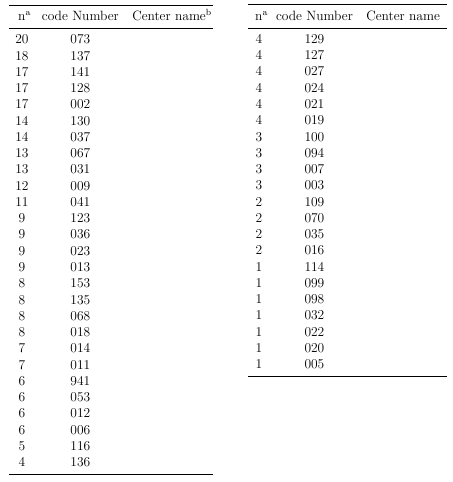
\includegraphics[width=0.80\textwidth]{tauladelscollons.png}
		\caption{\textbf{Centers at which eligible subjects were assessed at the baseline.} $| ^{a}.$ Number of subjects per center. $| ^{b}.$ We have been unable to find where the correspondence between center codes and center names is. However, the total number of centers can be found on the ADNI website.}
		\label{fig:tauladelscollons}
	\end{figure}
	\clearpage
	
	\subsection{The seven more frequent fMRI submodalities in our 332 eligible participants} \label{taula_submodalitats_fmri} 


		\begin{figure}[h]
			\centering
			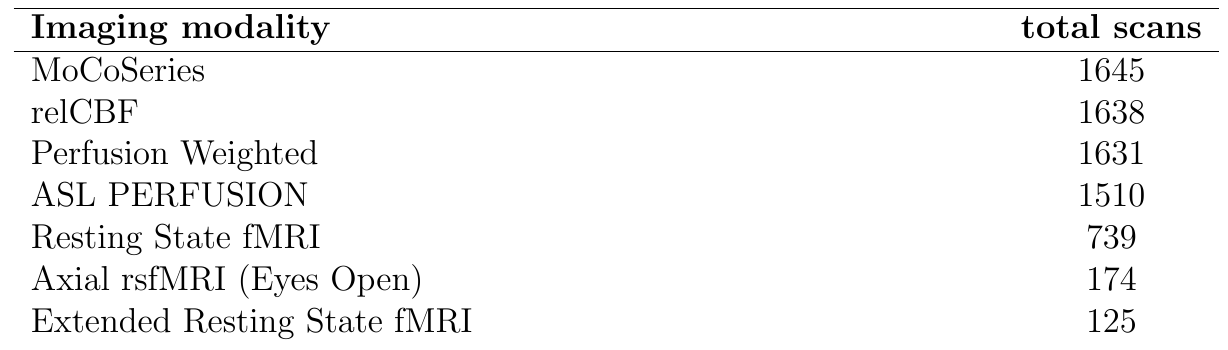
\includegraphics[width=1\textwidth]{fig_submodalitats_fmri_mesfrequents.png}
			\caption{\textbf{Value counts per submodality}, a measure of scan availability by fMRI subtype}
			\label{fig:submodalitats_fmri_mesfrequents}
		\end{figure}


	\subsection{Number of participants by site and group (results section)}\label{centres_resultats_74pacients}
		\FloatBarrier
		\begin{table}[h]
		\centering
		\begin{threeparttable}
			\caption{Number of participants and column percentages by site and group -final 74 patients sample-}
			\label{table:centres_en_mostrafinal_74 pacients}
			\begin{tabular}{ll|lll|llr}
				\toprule
				code n&site &MCI-c&MCI-nc&total&\% MCI-c&\% MCI-nc & $\sum$\%\\
				\midrule
				001&1&5&8&13&21,74&15,69&17,57\\
				130&53&4&7&11&17,39&13,73&14,86\\
				006&22&2&8&10&8,7&15,69&13,51\\
				018&13&1&6&7&4,35&11,76&9,46\\
				053&31&1&5&6&4,35&9,8&8,11\\
				013&10&2&4&6&8,7&7,84&8,11\\
				012&9&2&4&6&8,7&7,84&8,11\\
				006&4&3&3&6&13,04&5,88&8,11\\
				136&58&1&1&2&4,35&1,96&2,7\\
				129&52&0&2&2&0&3,92&2,7\\
				100&43&0&2&2&0&3,92&2,7\\
				019&14&1&1&2&4,35&1,96&2,7\\
				041&28&1&0&1&4,35&0&1,35\\
				\bottomrule
				&total&23&51&74&100&100&100\\
				\bottomrule
			\end{tabular}
			
			%\begin{tablenotes}
			%	\item[a]{asd}
			%	\item[b]{asd}
			%\end{tablenotes}
		\end{threeparttable}
	\end{table}
	
	
	
	

	\FloatBarrier
	
	
	
	\subsection{Homocedasticity and normality assumptions to support the use of statistical tests in demographics table and in FCon distribution comparisons.} \label{taula_levene_shapiro_demografics} 
	
		$H_{0}$ for \textit{shapiro wilk}: The null hypothesis, for this test, means that 
		the population of the corresponding subgroup (either MCIc or MCInc),
		for the given variable, is normally distributed. If + appears means that 
		we have to reject the Ho and thus the variable does not ajust a normal 
		distribution for that group.
		
		$H_{0}$ for \textit{levene test}: There is homogeneity of variances (both groups have
		same variance), for a given variable. If ``+'' symbol appears in figure \ref{fig:fig_shapiro_levene_taulaDEMOGRAFICS} below, it means that 
		we reject the Ho and therefore both groups are assumed not to 
		have the same variance.
		
		Thus, any variable (line) with any significant test result needs 
		the nonparametric option (Mann Whitney) [mw] instead of the parametric
		one (independent samples t-test) [t]:
		\FloatBarrier	
		\begin{figure}[h]
			\centering
			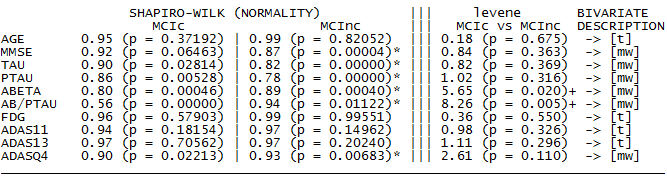
\includegraphics[width=1\textwidth]{fig_shapiro_levene_taulaDEMOGRAFICS.png}
			\caption{Assessment of the assumptions of all bivariate comparisons made in table \ref{table:demografics_biomarc_clinic_participants}.}
			\label{fig:fig_shapiro_levene_taulaDEMOGRAFICS}
		\end{figure}
		\FloatBarrier	

		Similarly, when comparing FC distributions between MCI-c and MCI-nc individuals (on the whole sample and by center), we have used the same tests to check the homocedasticity and normality assumptions before deciding which test to use. These were the results:
	
		\FloatBarrier
		\begin{figure}[h]
		\centering
			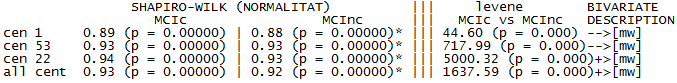
\includegraphics[width=1\textwidth]{fig_shapiro_levene_FCon.png}
			\caption{Assessment of the assumptions of all bivariate comparisons made in table \ref{fig:FCon_resultats}.}
			\label{fig:fig_shapiro_levene_FCon}
		\end{figure}
		\FloatBarrier
		\clearpage	
		
		
		
\section{Figures}

	\subsection{Unsuccessful models for functional connectivity without dimensionality reduction: ROC and Confusion matrices}\label{sec:fig_NaiveBayes_fMRI_nodimreduc_CONFUSIONiROCCURVE}

	
	\FloatBarrier
	%NAIVE BAYES ROC CURVE I CONFUSION MATRIX
	\begin{figure}[h]
		\centering
		\begin{minipage}{.5\textwidth}
			\centering
			\includegraphics[width=1\linewidth]{fig_GNB_fmri_nodimreduc_CONFUSION.png}
			\captionof{figure}{Naive Bayes confusion matrix.}
			%\label{fig:test1}
		\end{minipage}%
		\begin{minipage}{.5\textwidth}
			\centering
			\includegraphics[width=1\linewidth]{fig_GNB_fmri_nodimreduc_ROC.png}
			\captionof{figure}{Naive Bayes ROC curve.}
			%\label{fig:test2}
		\end{minipage}
	\end{figure}


	\FloatBarrier


	\begin{figure}[h]
		\centering
		\begin{minipage}{.5\textwidth}
			\centering
			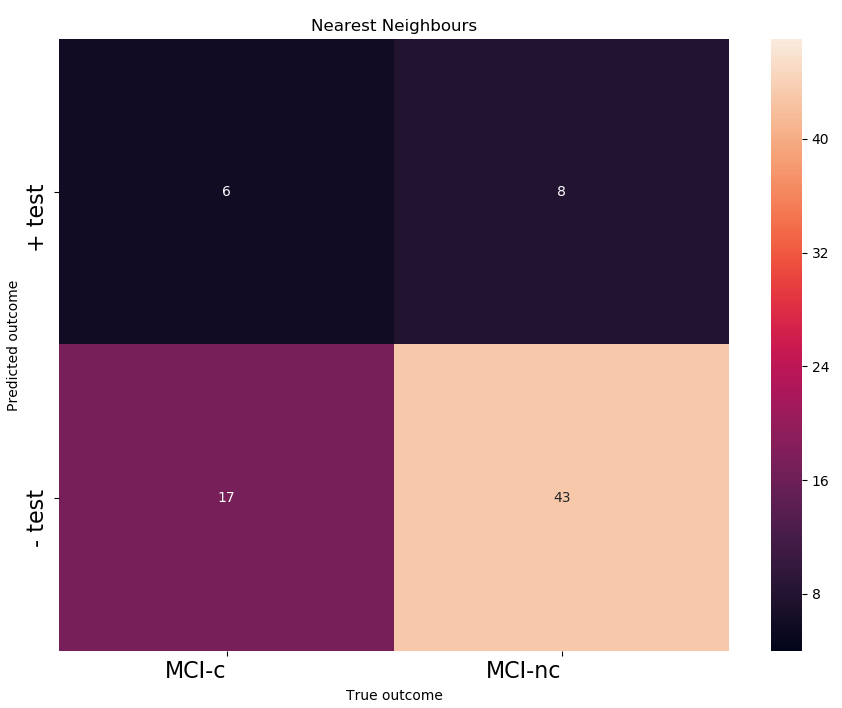
\includegraphics[width=1\linewidth]{fig_NN_fMRI_nodimreduc_CONFUSION.png}
			\captionof{figure}{Nearest Neighbours confusion matrix.}
			%\label{fig:test1}
		\end{minipage}%
		\begin{minipage}{.5\textwidth}
			\centering
			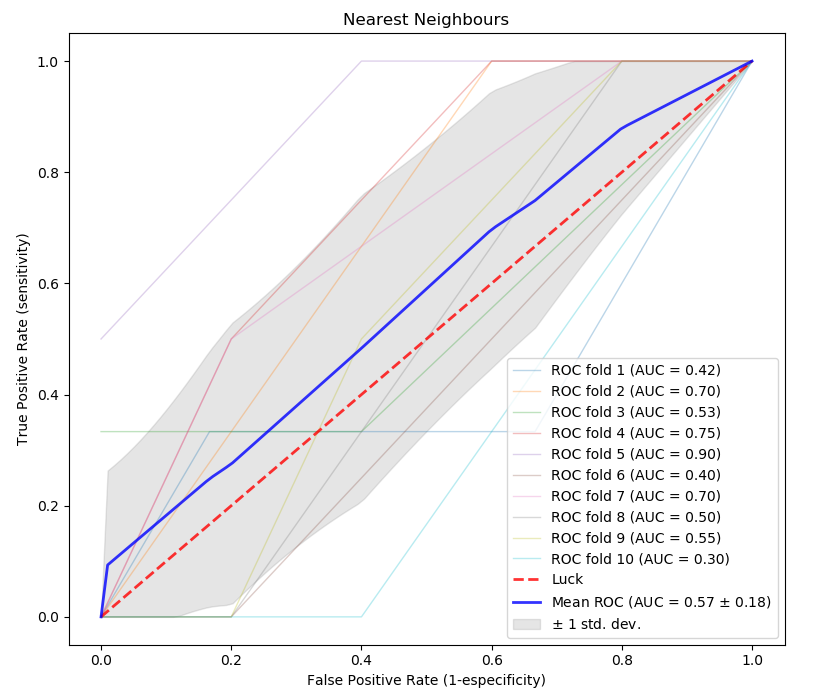
\includegraphics[width=1\linewidth]{fig_NN_fMRI_nodimreduc_ROC.png}
			\captionof{figure}{Nearest Neigbours ROC curve.}
			%\label{fig:test2}
		\end{minipage}
	\end{figure}





	\FloatBarrier
	
	\clearpage
	
	

	
	\subsection{Mean displacements for a randomly selected subject} \label{meandisplacements_registre}
		\FloatBarrier
		\begin{figure}[h]
			\centering
			\begin{subfigure}[a]{0.80\textwidth}
				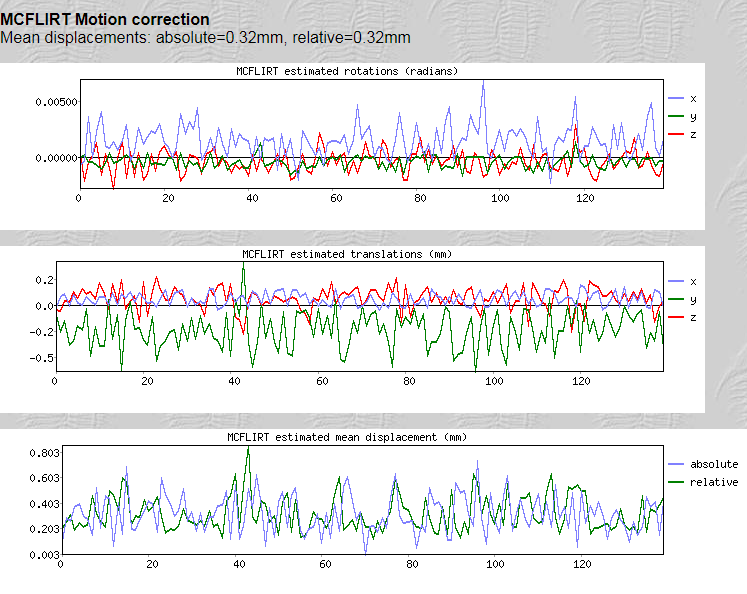
\includegraphics[width=1\textwidth]{fig_mean_displacements_annex.png}
				\caption{Preamble to motion-correction: Absolute mean displacement shows very good metrics.}
				\label{fig_mean_displacements_annex} 
			\end{subfigure}
			\begin{subfigure}[b]{0.80\textwidth}
				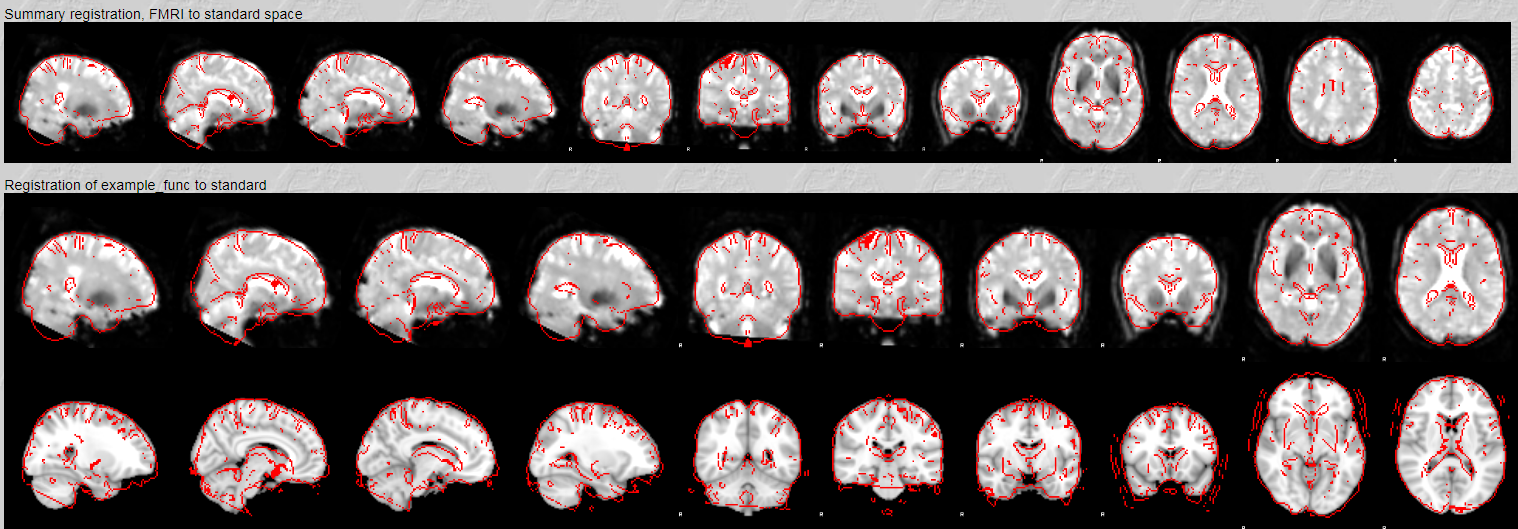
\includegraphics[width=1\textwidth]{fig_registre_cervellets.png}
				\caption{Registration information. GREY: Standard space. RED: the subject hereby considered. Both subjects are coincident.}
				\label{fig_registre_cervellets} 
			\end{subfigure}
			\caption{A randomly chosen subject from the 93 subjects whose fMRI scans were preprocessed using FSL.}
		\end{figure}
		\FloatBarrier
		\clearpage




	
		

\subsection{Functional connectivity matrices}\label{annex_functional_connectivities}

Here you can see the mean functional connectivity matrices across subject category (one for AD patients and the other for healthy controls), in the patients of the IDIBAPS clinic dataset (same dataset as \cite{Demirtas2017343}).


\begin{figure}[h]
	\centering
	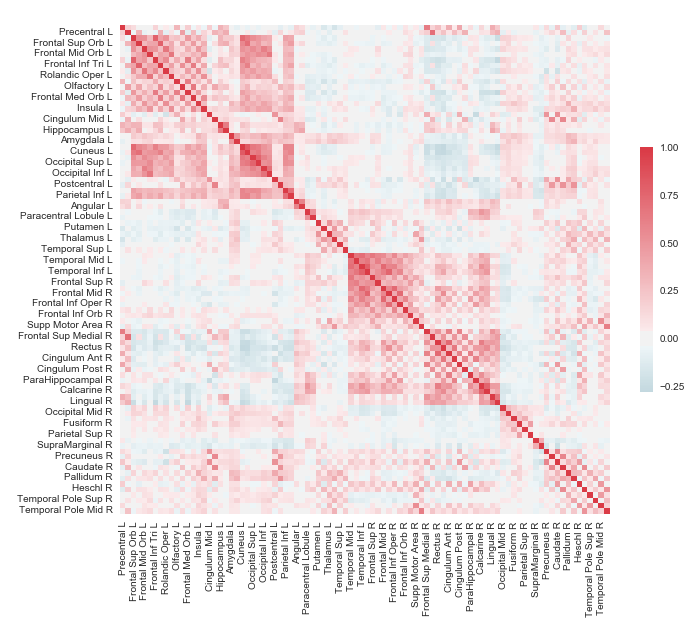
\includegraphics[width=\textwidth]{mitjana_ROIxROI_ALZHEIMER_ELIMINATS15PROBLEMATICS.png}
	\caption{Average correlation values for MNI AAL ROIs of Alzheimer disease patients}
\end{figure}


\begin{figure}[h]
	\centering
	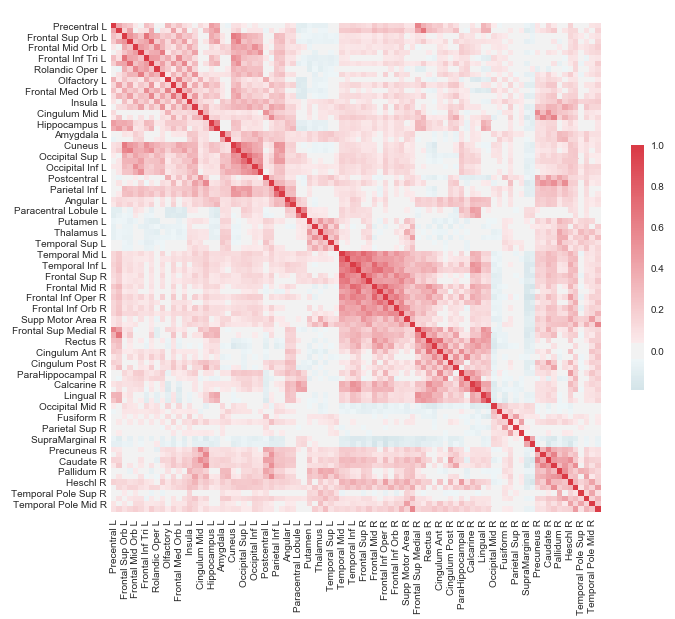
\includegraphics[width=\textwidth]{mitjana_ROIxROI_controls_ELIMINATS15PROBLEMATICS.png}
	\caption{Average correlation values for MNI AAL ROIs of healthy control patients}
\end{figure}


%REPORTING

\clearpage






	\section{Depicting the method of unique scan selection in subjects with more than one rsfMRI the same day} \label{escollir_escaners_repetits_dun_mateix_dia}

As we said, seven subjects had several scans in the same day: from these scans only one was to be chosen in order to test our hypothesis. We chose the best one according to the following criteria applied to figure \ref{fig:escans_exclosos}: 

BOLD:  Chosen scan $|$ CROSSED OUT: Excluded scan $|$ NO EMPHASIS: Scan eligible but not chosen because was not deemed to be the the most optimal.



\FloatBarrier
\begin{figure}[h]
	\centering
	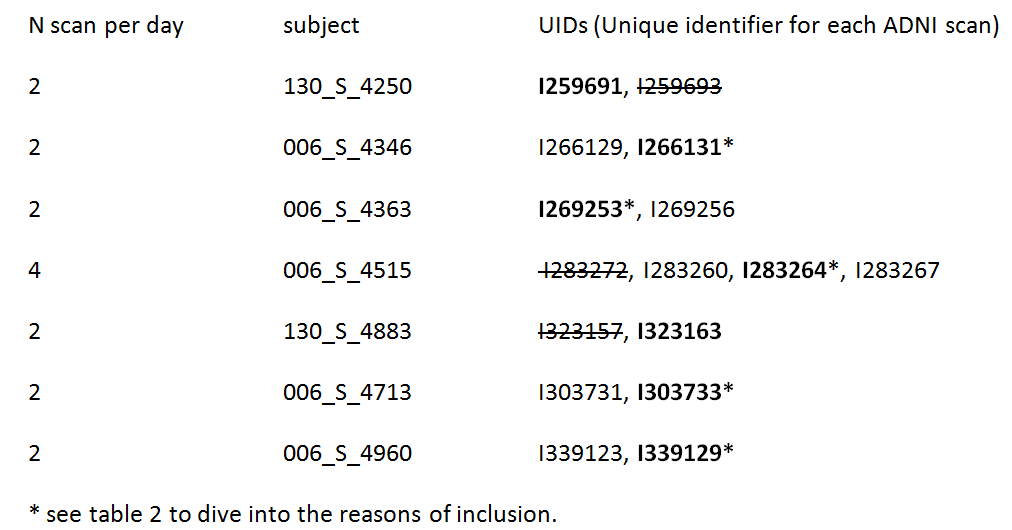
\includegraphics[width=\textwidth]{fig_escans_exclosos.png}
	\caption{Number of repeated rsfMRI scans in the same day, by subject and UID.}
	\label{fig:escans_exclosos}
\end{figure}
\FloatBarrier


The reasons why we directly excluded the scans that appear crossed out in figure \ref{fig:escans_exclosos} are:

a)	The scan was not completed (i.e. the scan had less than the number of time series –in this case 140- all the other subjects had): These is the problem found with I323157 and I283272 from subjects 130\_S\_4883 and 006\_S\_4515 respectively.

b)	FSL did not process the scan properly and did not even obtain an output file. The error shown on screen was ``WARNING:: Inconsistent orientations for individual images when attempting to merge'' and ``Error in size-match along non-concatenated dimension for input file:''  (besides in this case the scan did not even have information of fMRI adquisition parameters as an .xml file, whereas scans in the ADNI have a corresponding .xml file with those parameters). This  scan is I259693, corresponding to subject 130\_S\_4250. 

Sometimes exclusion was not straightforward, since several scans, apparently, were valid candidates to represent the functional connectivity of a given subject. Thus, for each of those given subjects,  we simply chose the representing scan based on a criteria of minimizing the absolute and relative mean displacements as showed in the “report.html” file Melodic obtains for each subject that the software preprocesses. This is the case for  the subjects  006\_S\_4346,  006\_S\_4363,  006\_S\_4713,  006\_S\_4960. For this subjects we provide the mean displacements as follows in figure \ref{fig:escans_displacements}:


\FloatBarrier
\begin{figure}[h]
	\centering
	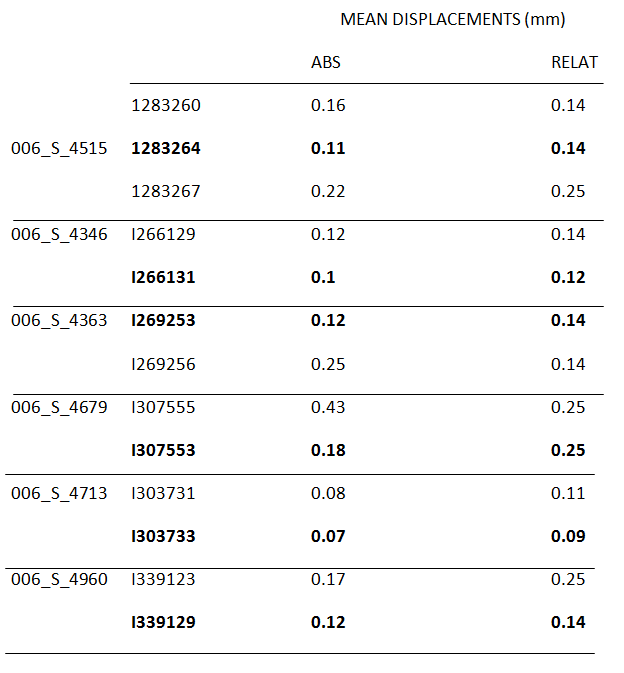
\includegraphics[width=0.8\textwidth]{fig_escans_displacements.png}
	\caption{NOTE: Mean absolute and relative displacements for scans of subjects taken in the same day. One scan was selected per each subject for having the lowest mean displacements. $|$ \textit{NOTE: Although scan I259691 did not have fMRI adquisition parameters as an .xml, it was not excluded. We assumed same parameters as other scans.}}
	\label{fig:escans_displacements}
\end{figure}
\FloatBarrier
\clearpage















\section{Reporting: EQUATOR guidelines} \label {equator_guidelines}

\subsection{Creating a tailored guideline for our study}
In this final thesis I chose the {TRIPOD checklist, in its prediction model development and validations version}, to report my results (\href{https://bit.ly/2HU58V5}{click here} to see them \footnote{or copy the following footnote adress https://bit.ly/2HU58V5}). However, since this study has some particularities that regular prognostic studies do not have, some features were uncovered and not asked to be reported. 

To overcome this limitation, I decided to add three extra guidelines. First, the STARD guidelines, that are used in diagnostic studies; Second, the MLBS guidelines\footnote{These guidelines do not have an oficial abreviation. We have created one that stands for Machine Learning in the Biomedical Sciences.}, to report correctly the created machine learning models in our study, since their complexity makes it harder to convey good reporting; and finally, the RECORD guidelines, in order to properly specify the process of obtaining the information from a database fed with routinely collected data from observational studies (the ADNI belongs to that category, since it is a cohort study with regular follow-ups).

The EQUATOR links for the guidelines used can be found and explained in the following table:

\begin{center}
	\begin{table}[h] 
		\begin{tabular}{m{3cm} m{9.8cm}}
			\hline
			\textbf{Guideline\newline abbreviation} & \textbf{repoting\newline aim}\\
			\hline
			\href{http://www.equator-network.org/reporting-guidelines/tripod-statement/}{TRIPOD} & Studies developing, validating, or updating a prediction model, whether for diagnostic or prognostic purposes.\\
			\hline
			\href{http://www.equator-network.org/reporting-guidelines/stard/}{STARD} & Diagnostic accuracy studies\\
			\hline
			\href{http://www.equator-network.org}{RECORD} & Reporting items specific to observational studies using routinely collected health data.\\
			\hline
			\href{http://www.equator-network.org/reporting-guidelines/guidelines-for-developing-and-reporting-machine-learning-predictive-models-in-biomedical-research-a-multidisciplinary-view/}{MLBS}$^{***}$ & Machine learning predictive models in biomedical research\\
			
			\hline	
		\end{tabular}{}
		\caption{EQUATOR guidelines that have been used for reporting this pronostic study. $^{***}$ \textit{These guidelines do not have an oficial abreviation. We have created one, that stands for Machine Learning in the Biomedical Sciences}}
	\end{table}
\end{center}

%\section{Codes and syntaxis files} 

%In this section python code can be followed to see how we approached the data analysis. We have not been exhaustive in all the functions shown, because the list of codes has several files. This is just for display the most relevant parts of the code.


%\subsection{finding NaNs within a 3D tensor}\label{codis}
%\lstinputlisting[language=python]{inputlatexprovapython.py}


%\subsection{main function for analysis}
%\lstinputlisting[language=python]{./copiescodi/funcionsauxiliars.py}



\section{Director/tutor final thesis certificate} \label{director}

\FloatBarrier
\begin{figure}[h]
	\centering
	
\includegraphics[width=1\textwidth]{fig_certificat_tutoridirector.png}
	\label{fig:tutordirector}
\end{figure}
\FloatBarrier
\clearpage





















%definim la bibliografia (xucla de paquet natbib)
\bibliographystyle{vancouver} %" estil vancouver!!
\clearpage
\part{Bibliography}
\bibliography{bib-TFM-FINAL}  %posar aqui nom dl fitxer .bib que te les referencies
%________________________

\end{document}								